% Created 2026-10-04 日 13:20
% Intended LaTeX compiler: pdflatex
\documentclass[dvipdfmx, a4paper, 12pt]{jsarticle}

\usepackage[utf8]{inputenc}
\usepackage[T1]{fontenc}
\usepackage[dvipdfmx]{graphicx}
\usepackage{longtable}
\usepackage{wrapfig}
\usepackage{rotating}
\usepackage[normalem]{ulem}
\usepackage{amsmath}
\usepackage{amssymb}
\usepackage{capt-of}
\usepackage[dvipdfmx]{hyperref}
\setcounter{secnumdepth}{2}
\author{Shigeto R. Nishitani}
\date{\today}
\title{HyperCardを真似た論文作成directory構築}
\hypersetup{
 pdfauthor={Shigeto R. Nishitani},
 pdftitle={HyperCardを真似た論文作成directory構築},
 pdfkeywords={},
 pdfsubject={},
 pdfcreator={},
 pdflang={Jp}}
\begin{document}

\maketitle
\tableofcontents

\section{Introduction}
\label{sec:org2929f12}
\href{../d99\_junior\_ruby/readme.html}{prev\_button}
\href{../canvas.html}{up\_button}
\href{../d2\_divide\_chunk/readme.html}{next\_button}
\subsection{Introduction}
\label{sec:org162df6d}
HyperCardっていう面白いソフトが初期のMacには無料でついてました．
これは，GUI的なアプリの基本となってものです．
でも，みんなが使えるアプリにするために，
多くのいいところが削がれていきました．
皆さんに提供しようとするHyperCardアプリは
それを
"an essential software construction kit 
that belonged in the hands of everday users."
とすることを目的としています．

HyperCardではカードをまとめた"Stack"で
Diskに入れて交換されていました．
この授業では，院生，卒研生に利用してもらえる
Mock-Upと作りながら"HyperCard"のコンセプトを
理解してもらう予定です．

\begin{center}
\begin{tabular}{p{0.44\linewidth}p{0.44\linewidth}}
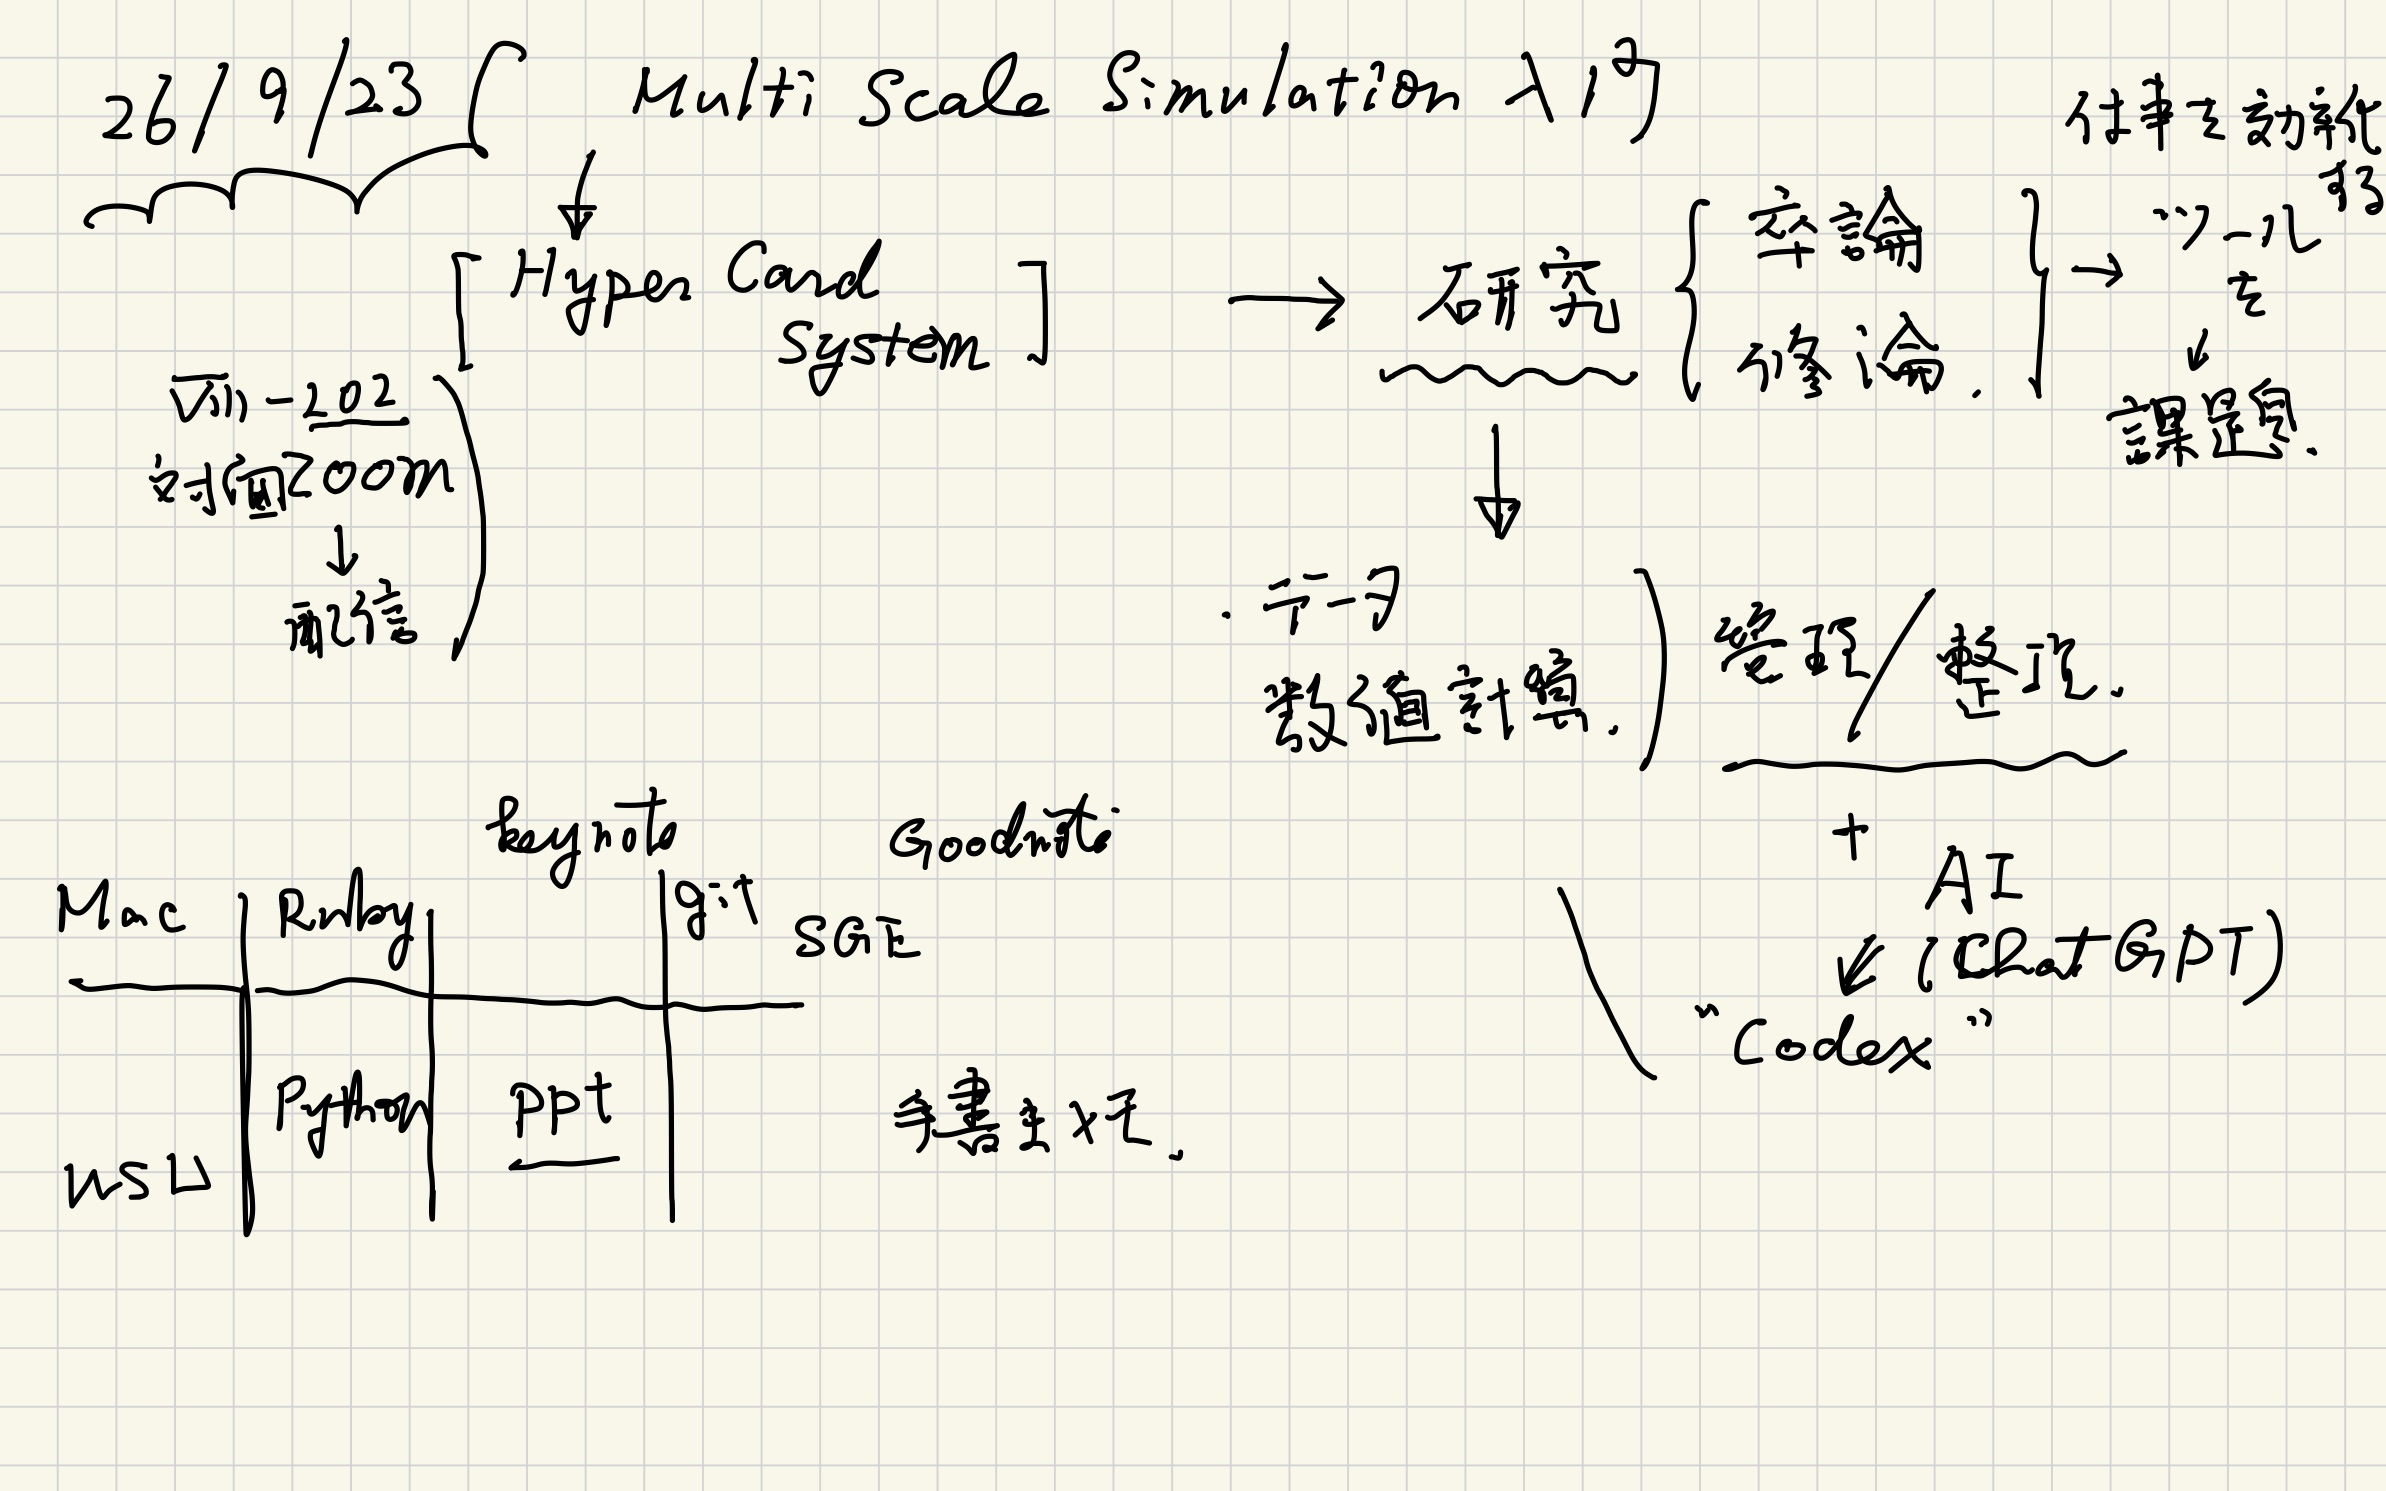
\includegraphics[width=\linewidth]{../d1_mock/figs/on_line_jpgs/multi_scale_26f-1.jpg} & 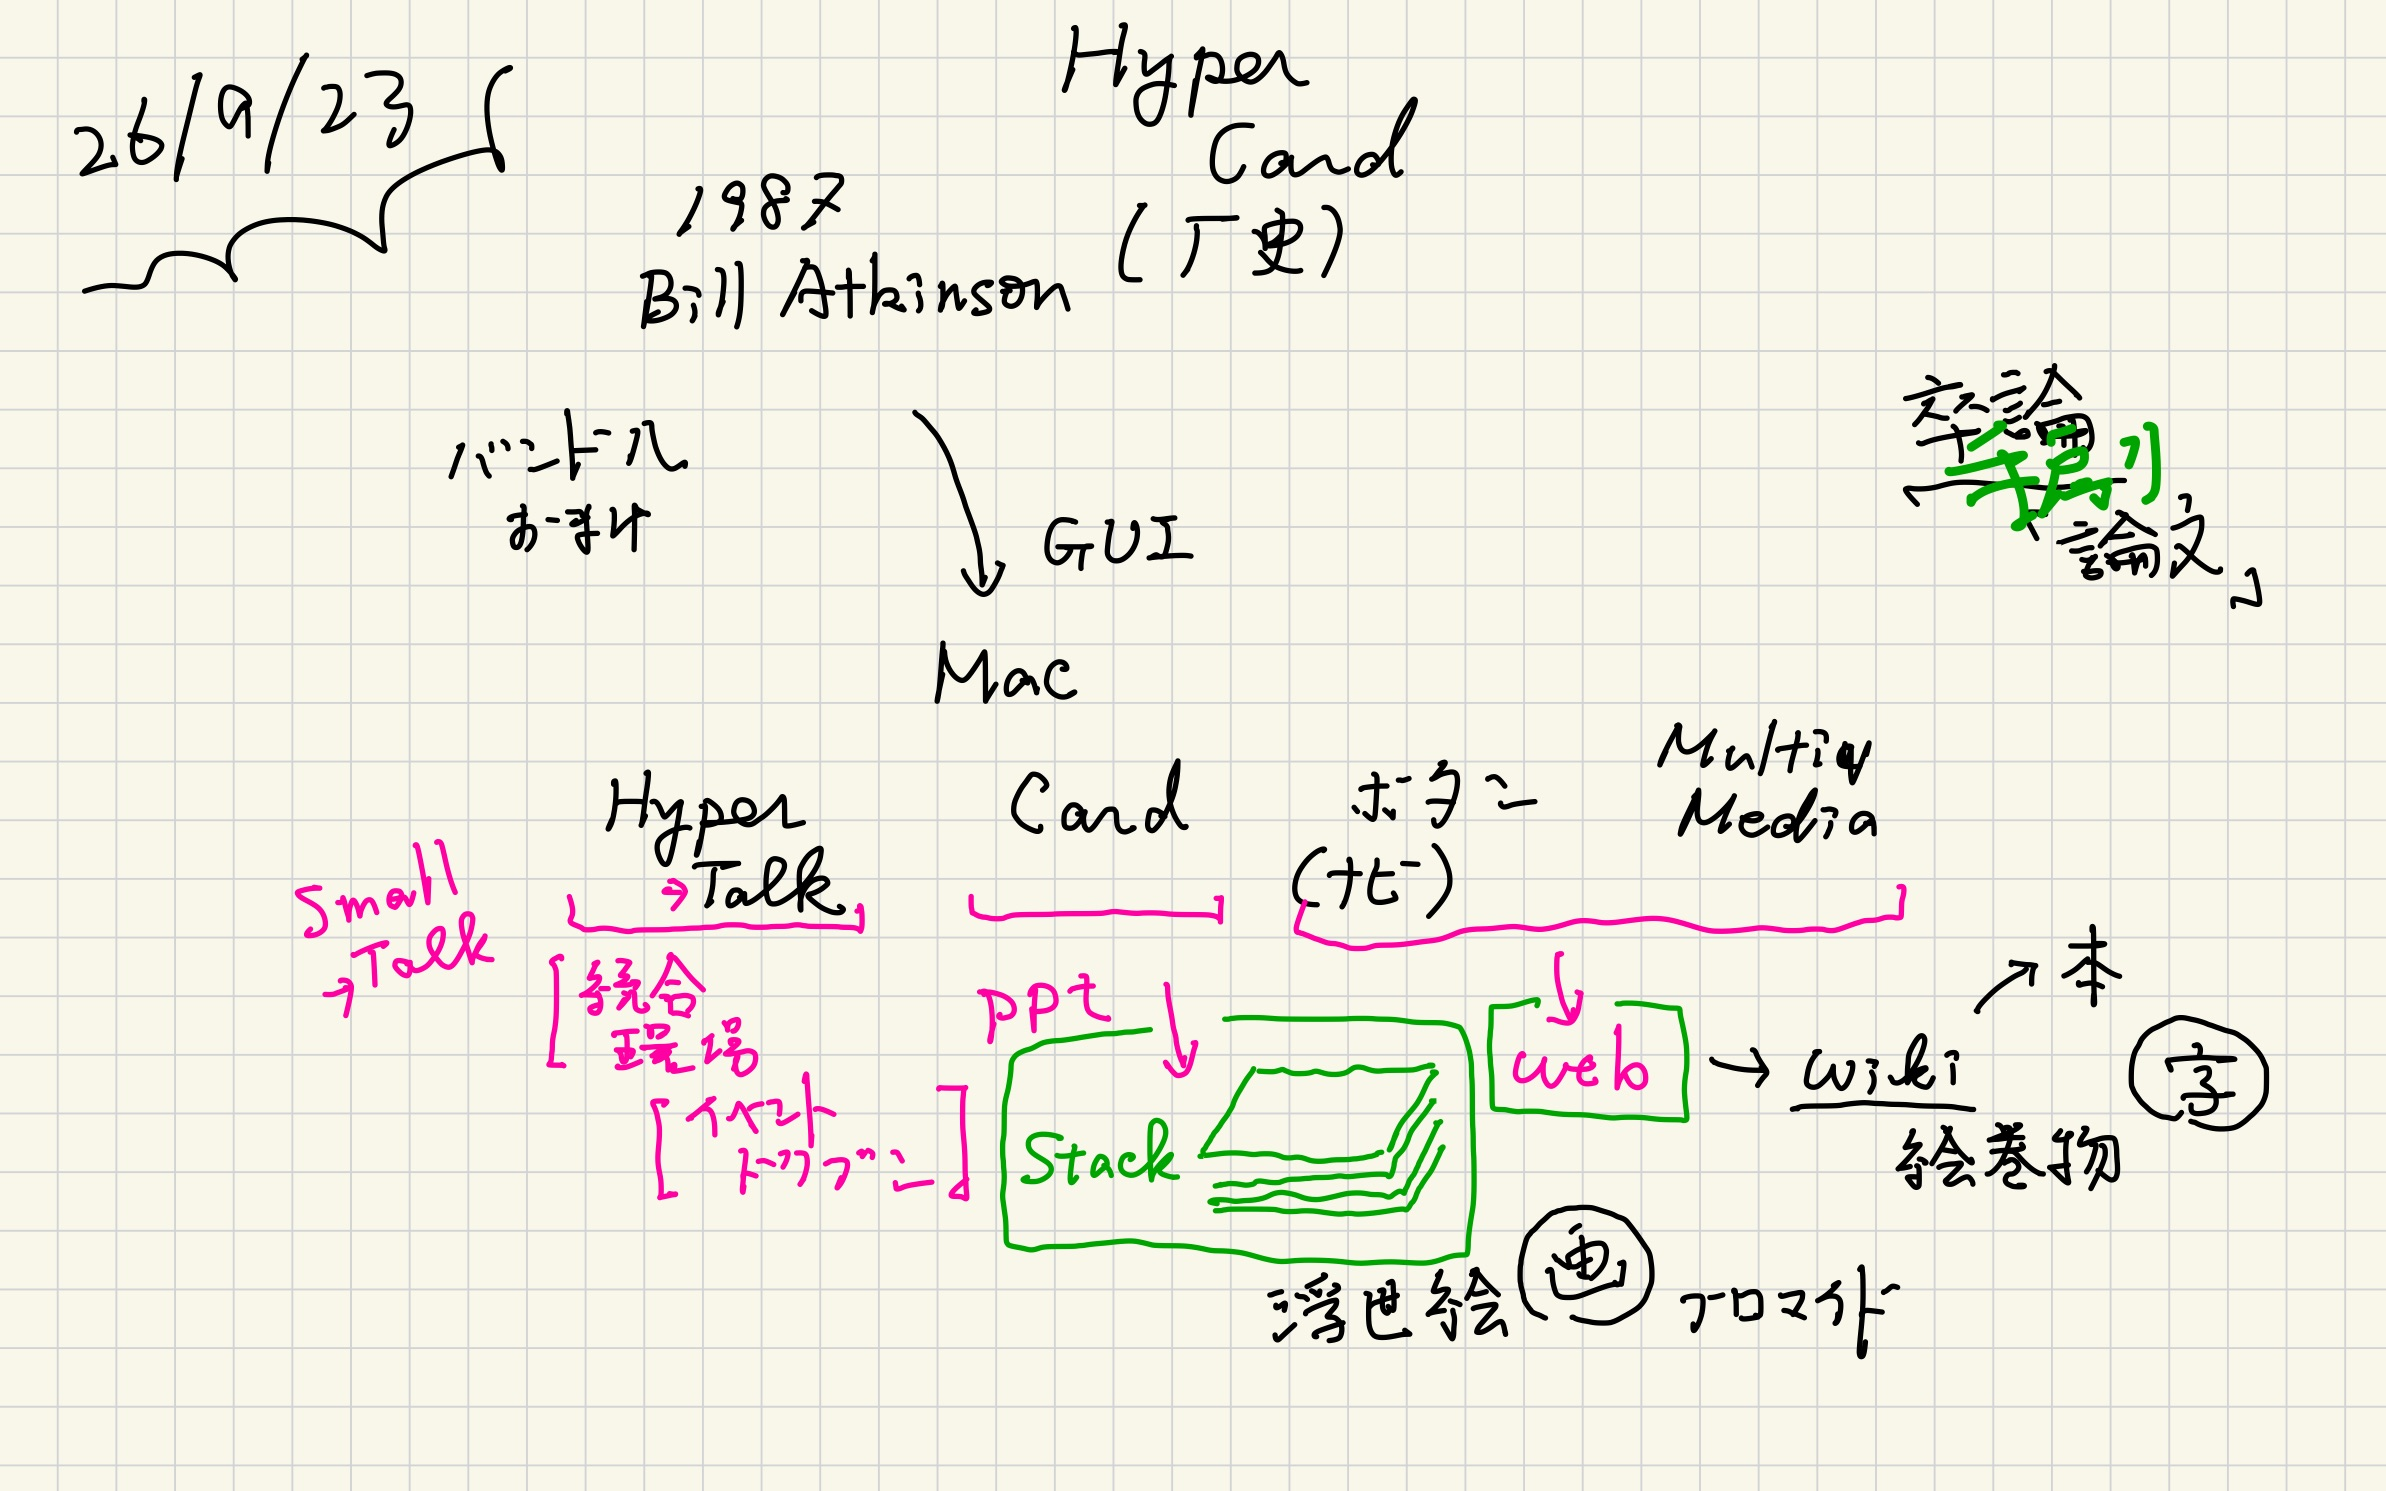
\includegraphics[width=\linewidth]{../d1_mock/figs/on_line_jpgs/multi_scale_26f-2.jpg}\\
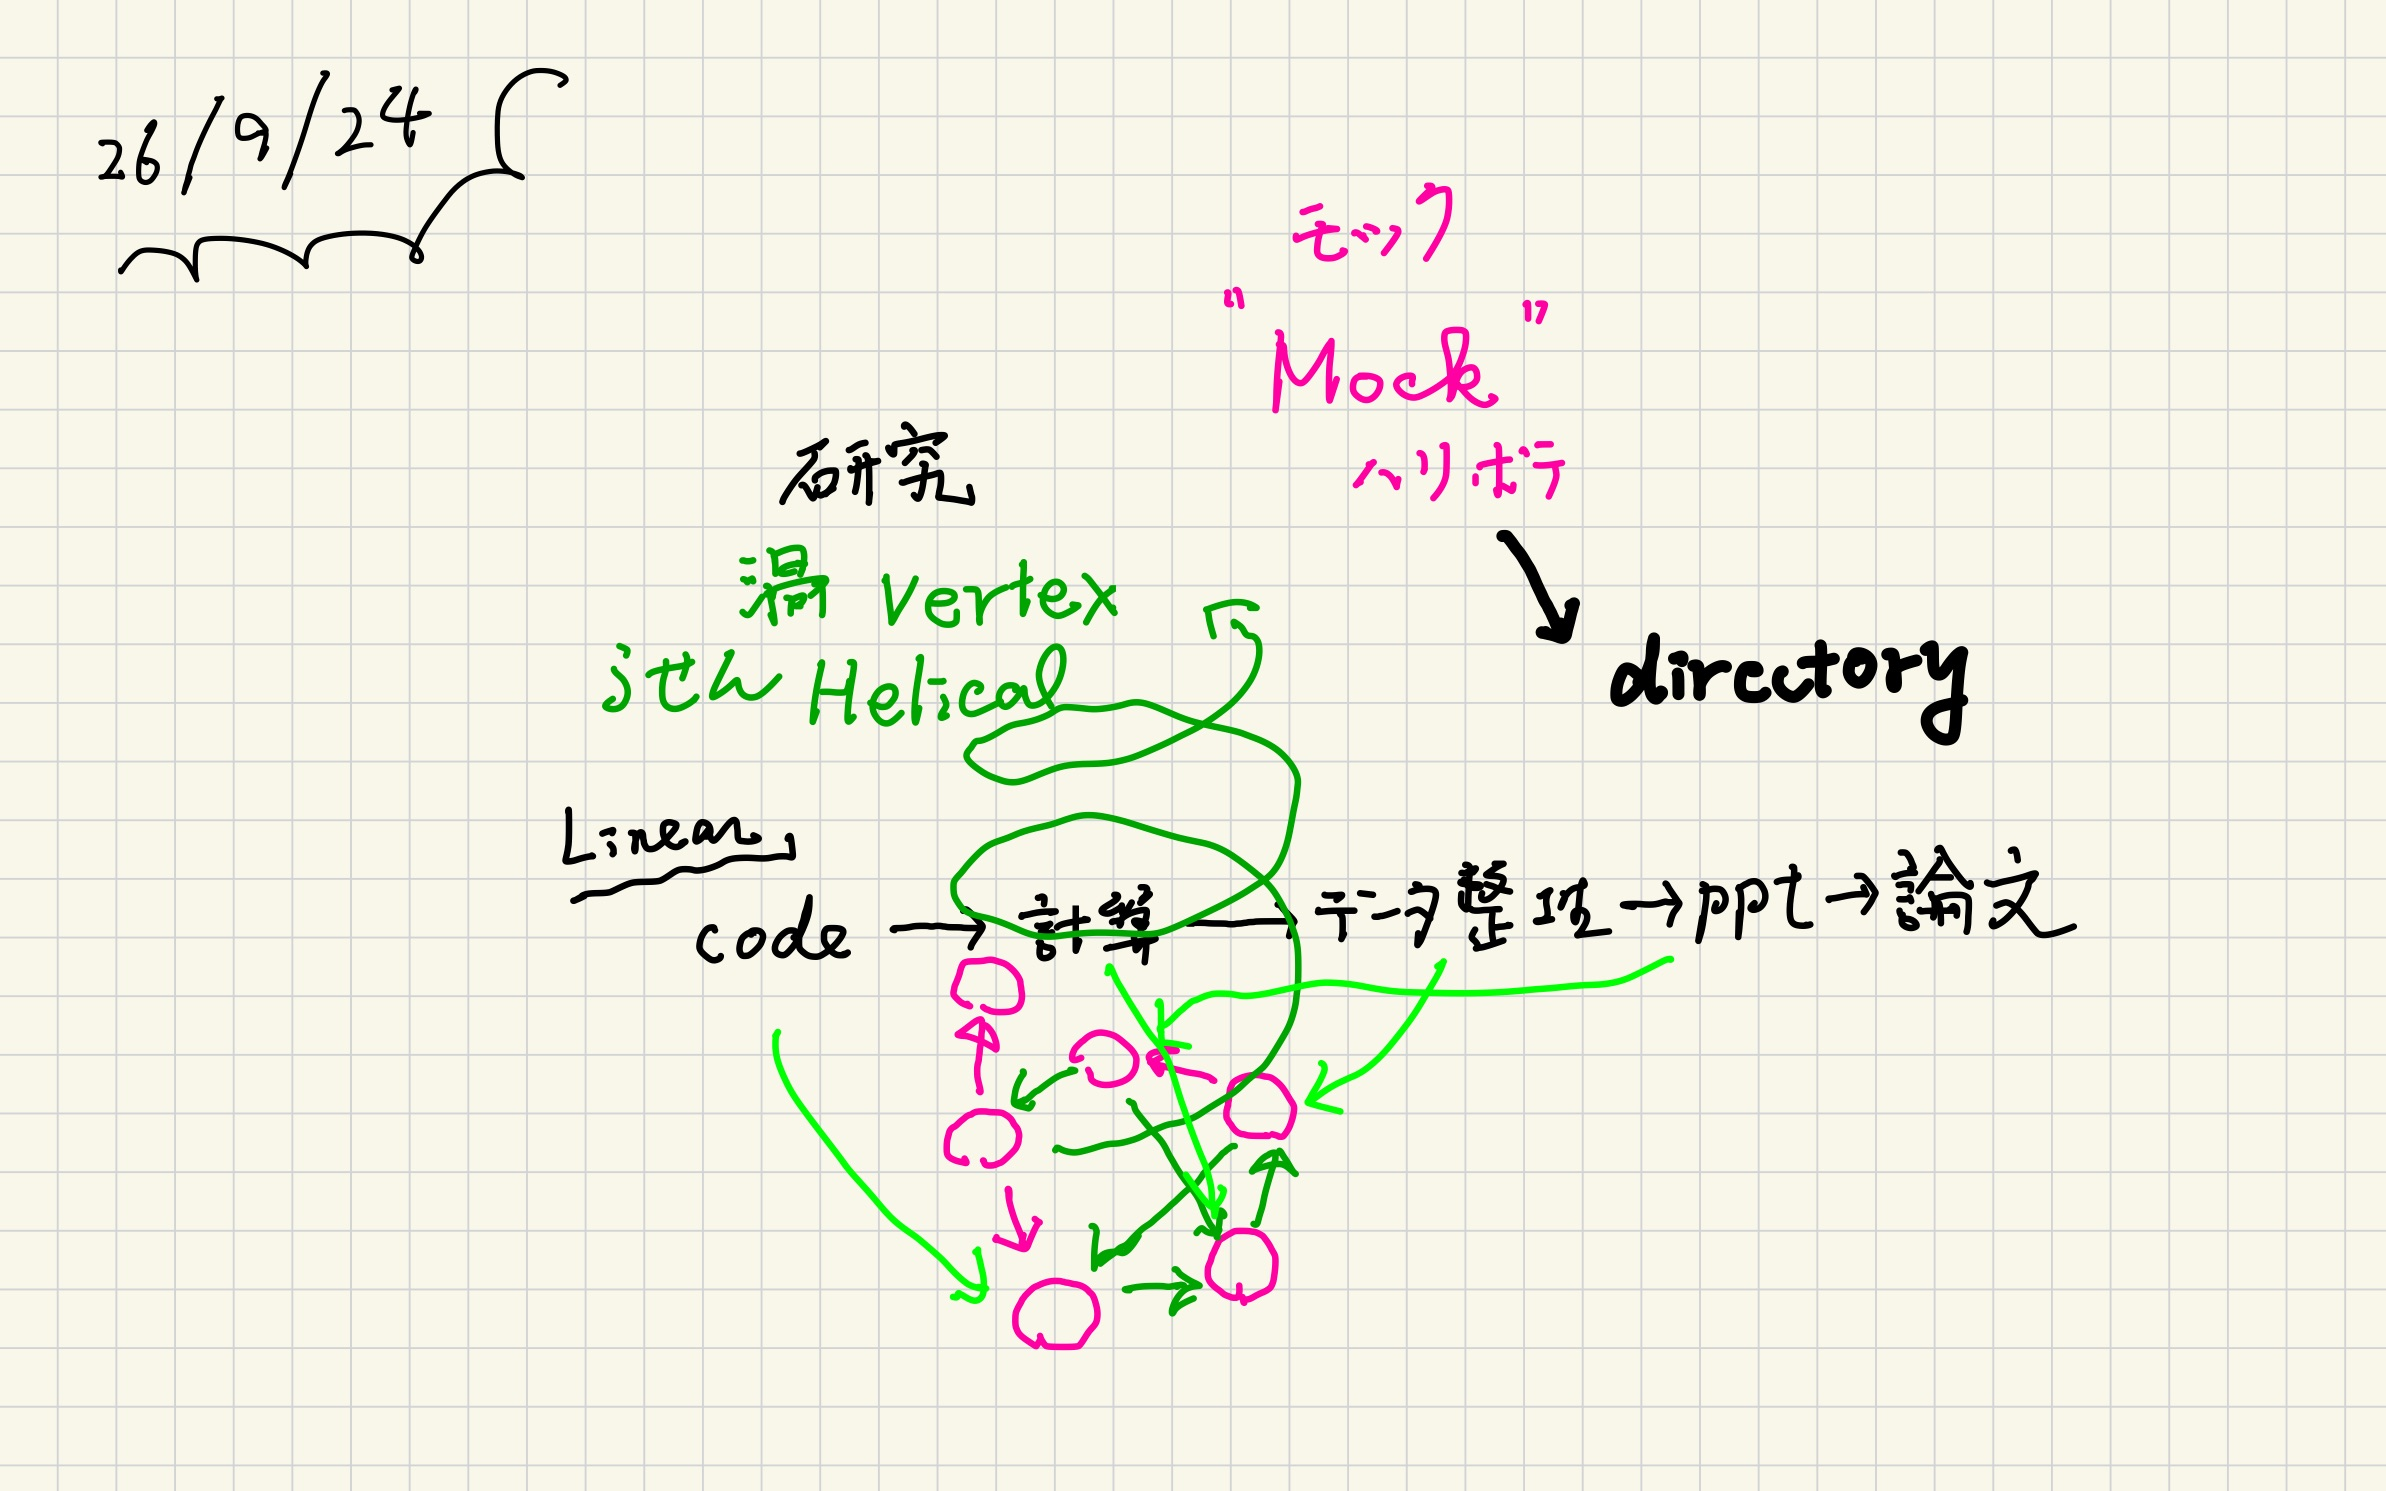
\includegraphics[width=\linewidth]{../d1_mock/figs/on_line_jpgs/multi_scale_26f-3.jpg} & 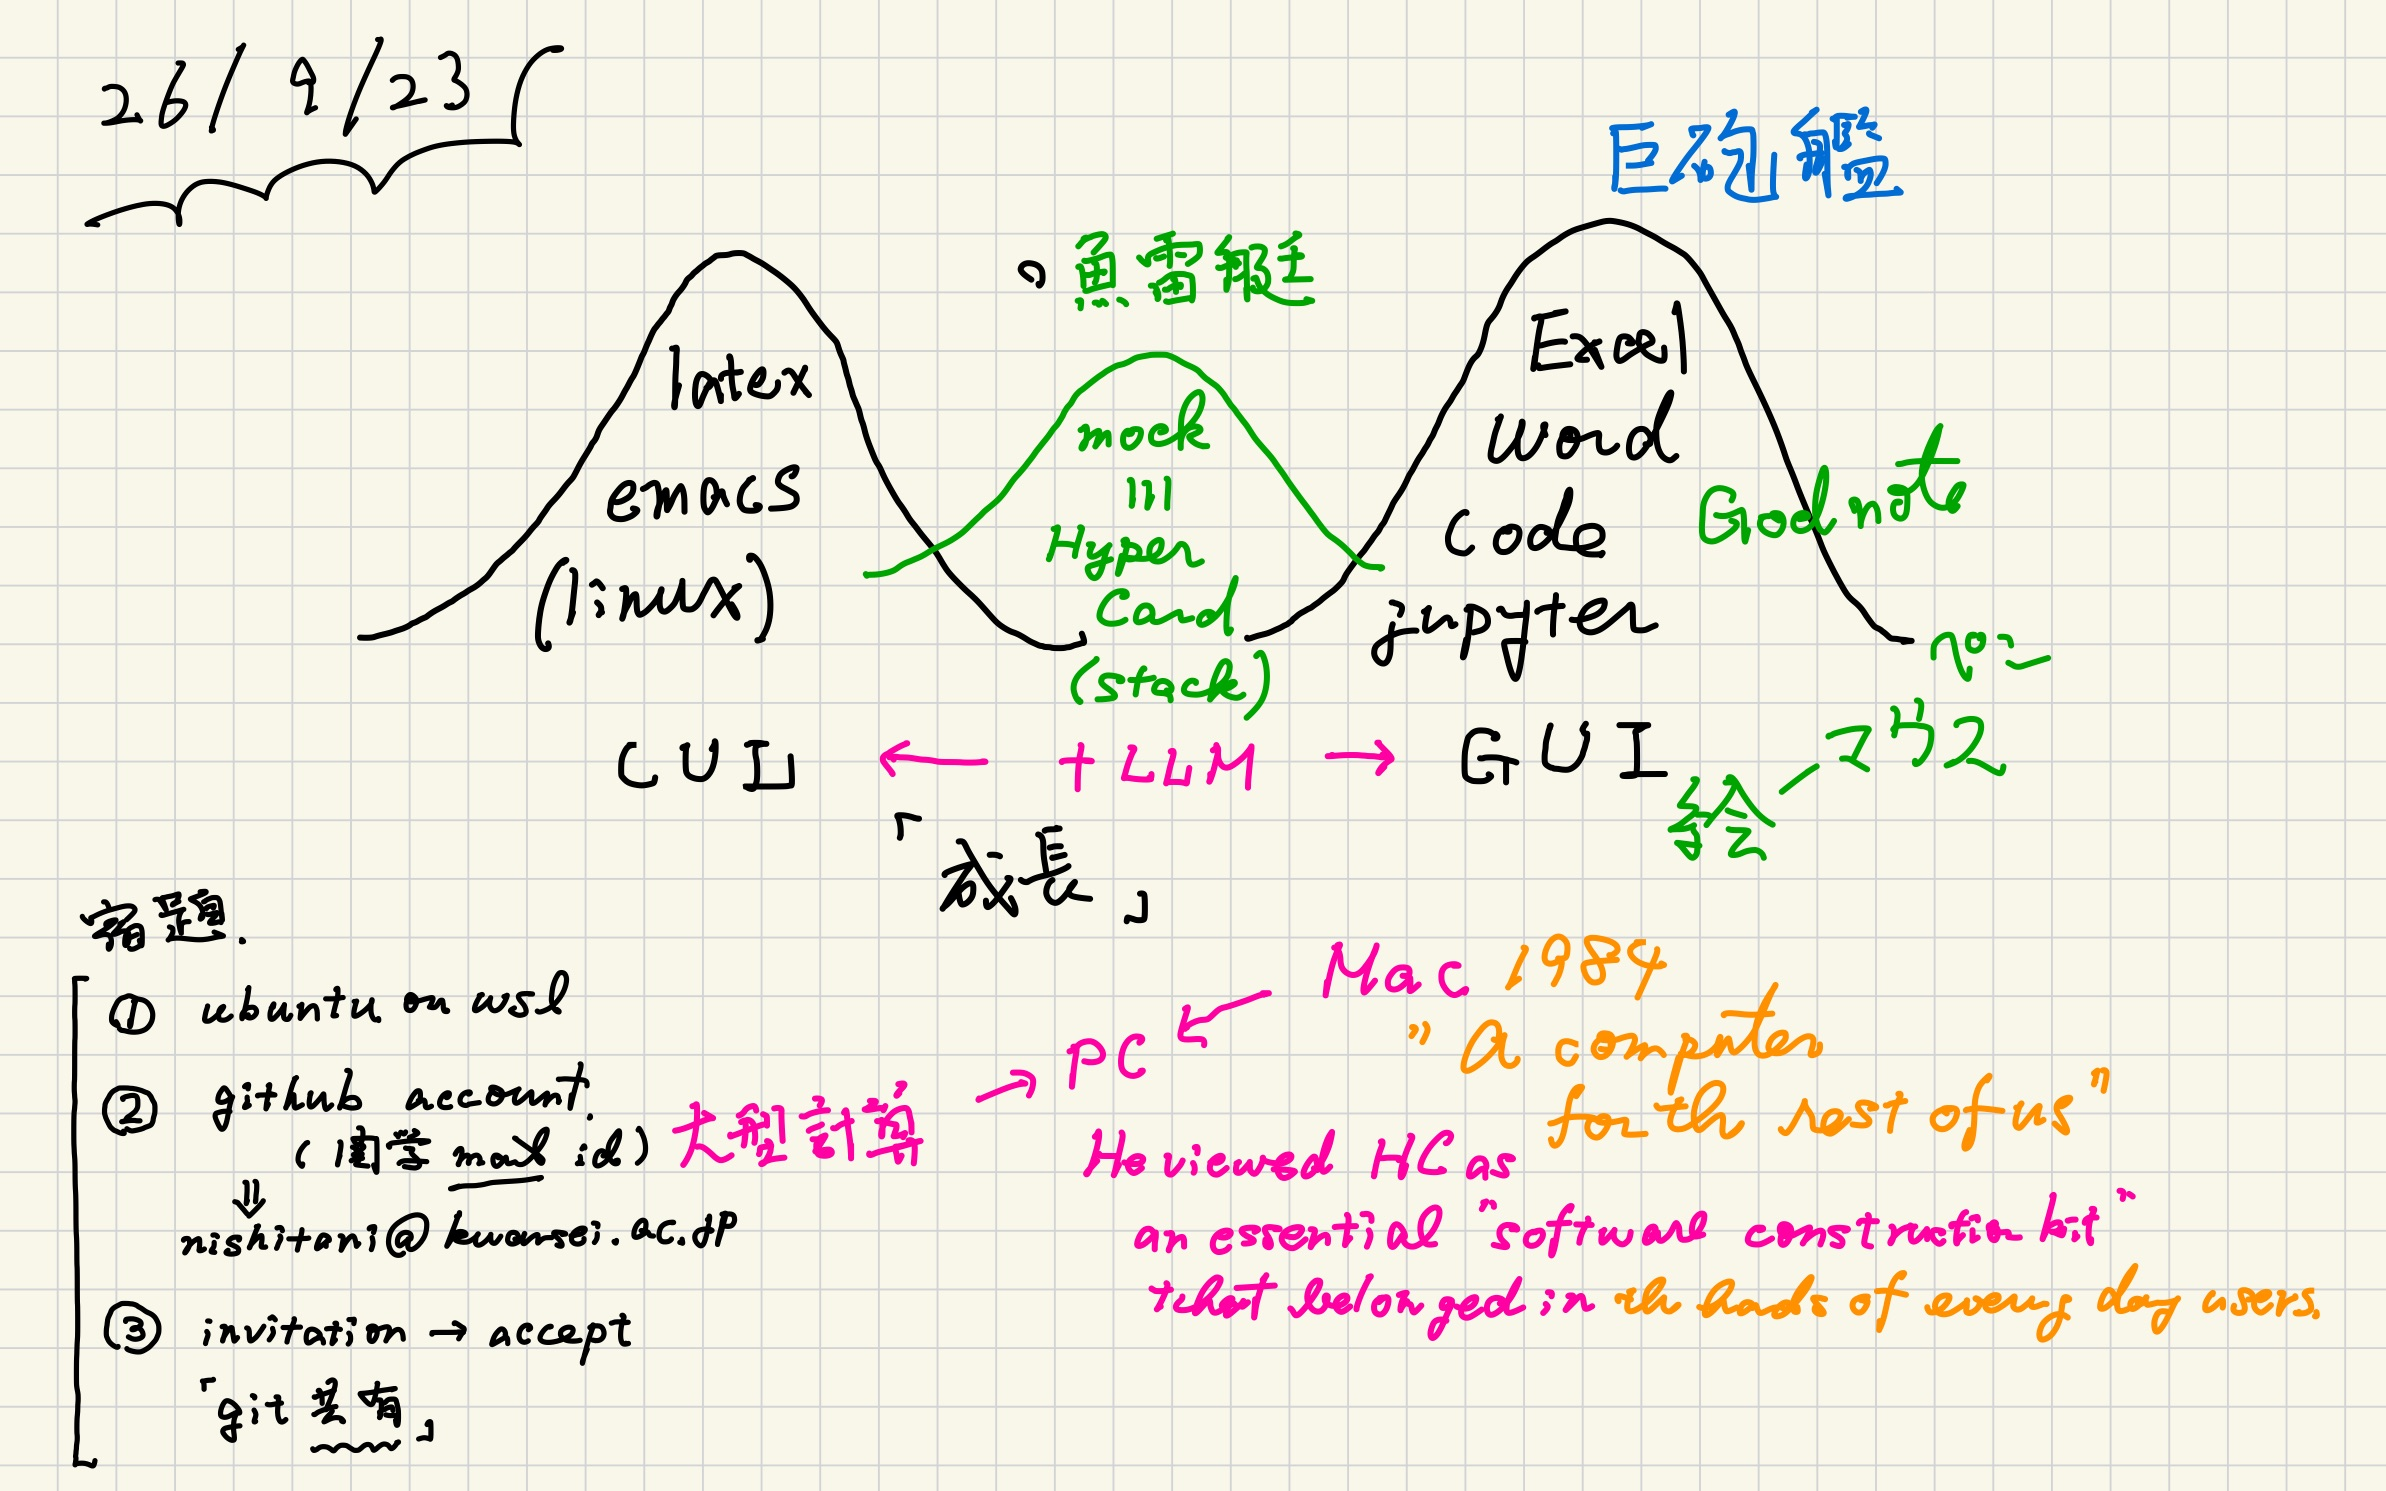
\includegraphics[width=\linewidth]{../d1_mock/figs/on_line_jpgs/multi_scale_26f-4.jpg}\\
\end{tabular}
\end{center}
\subsection{An example : jps\_26f}
\label{sec:org49f2f3a}
\begin{center}
\begin{tabular}{p{0.88\linewidth}}
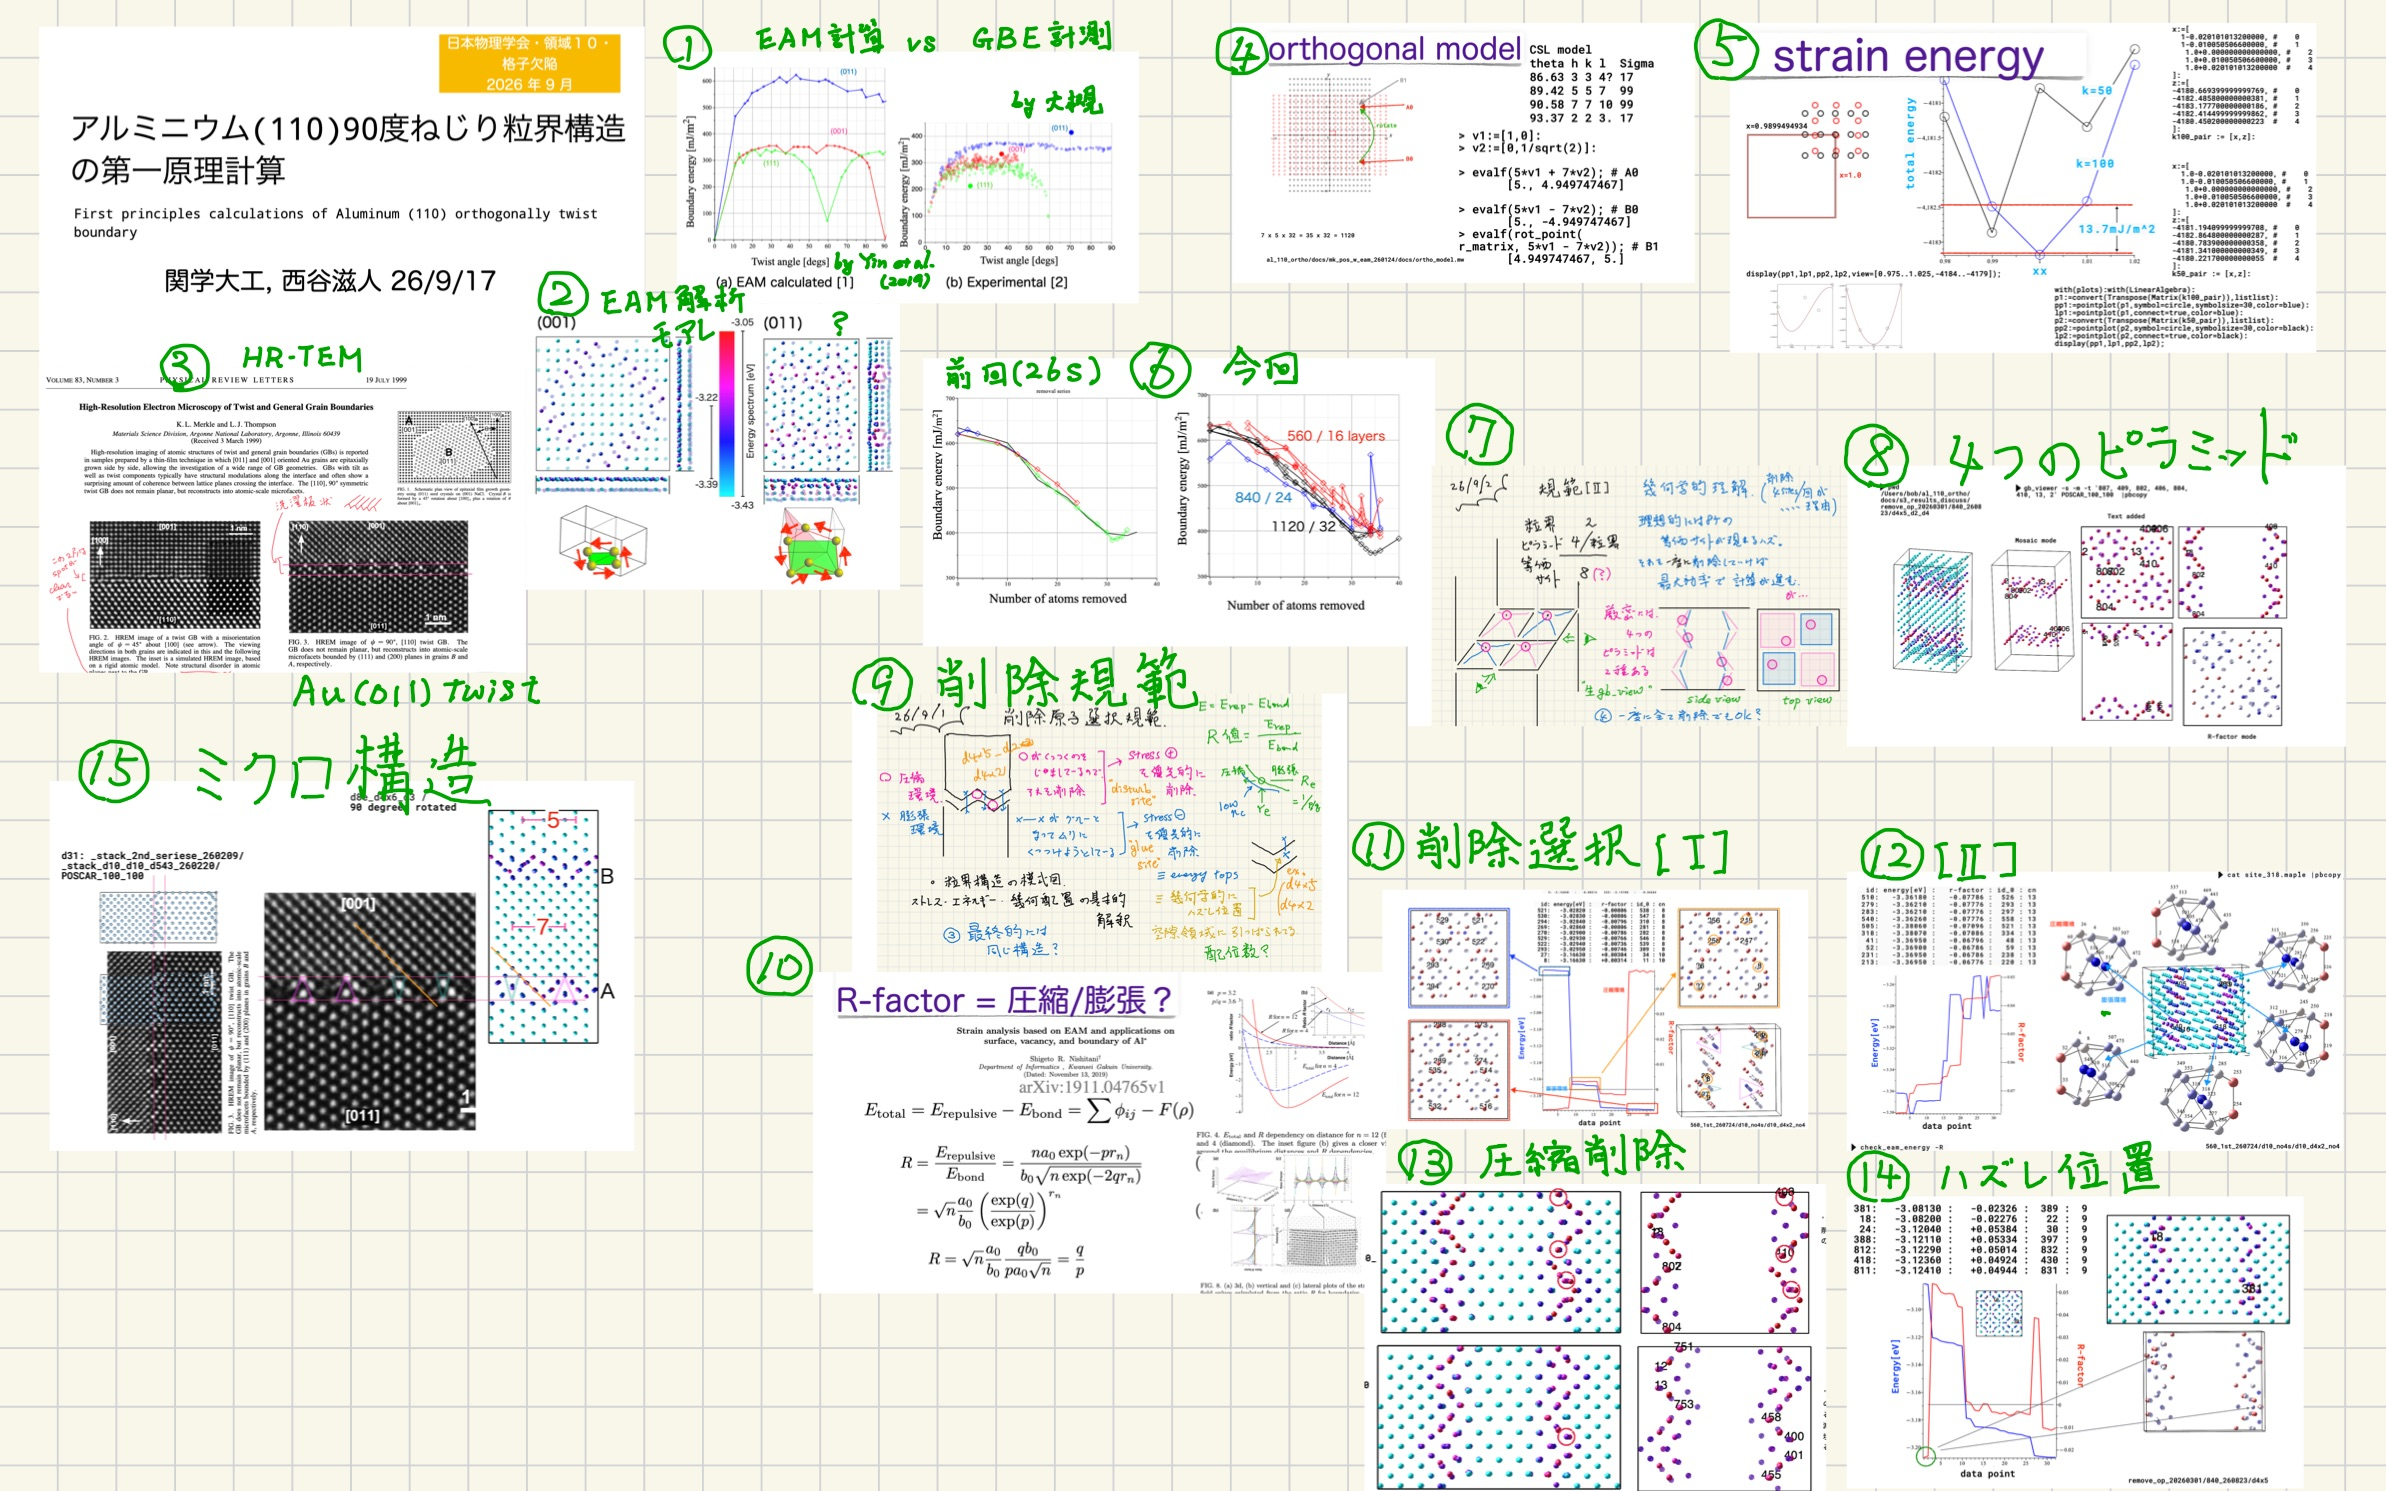
\includegraphics[width=\linewidth]{../d1_mock/figs/prepare_jpgs/hyper_card_system-94.jpg}\\
\end{tabular}
\end{center}

これは，9月に物理学会での発表のcardです．
これを作成するためのMock-Upを
みていきましょう．
\subsection{Preparation notes}
\label{sec:org83965d7}
\begin{center}
\begin{tabular}{p{0.293\linewidth}p{0.293\linewidth}p{0.293\linewidth}}
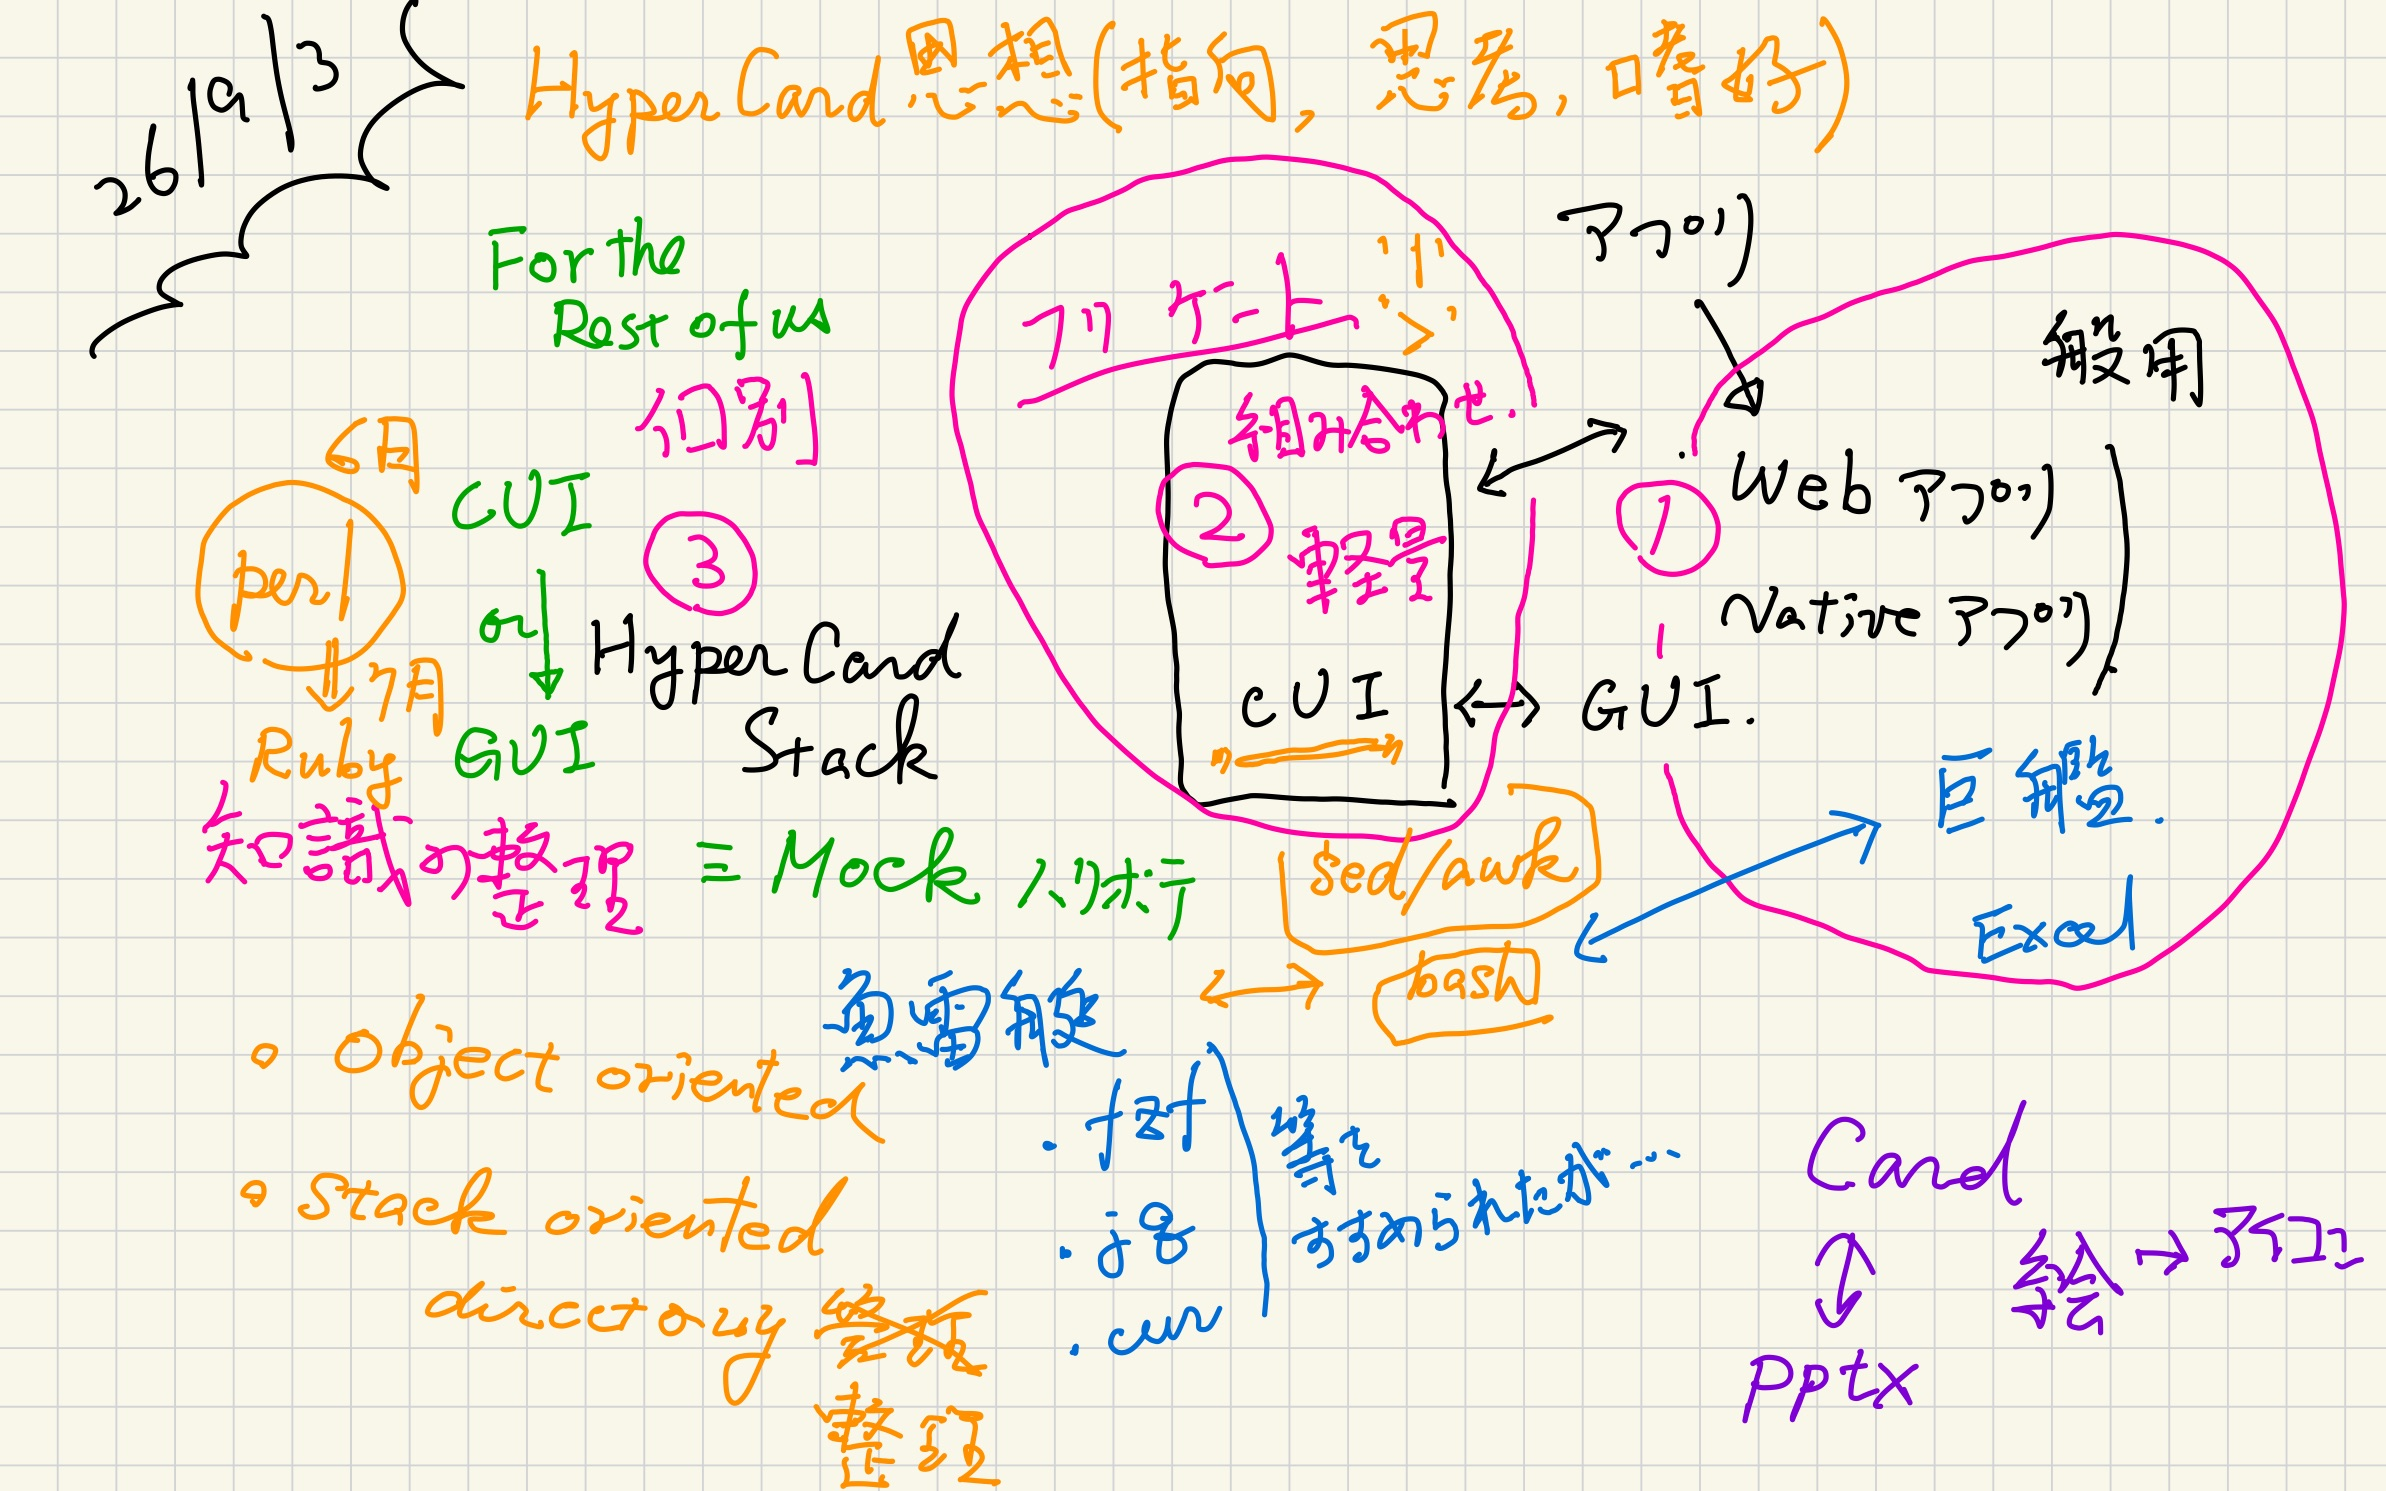
\includegraphics[width=\linewidth]{../d1_mock/figs/prepare_jpgs/hyper_card_system-89.jpg} & 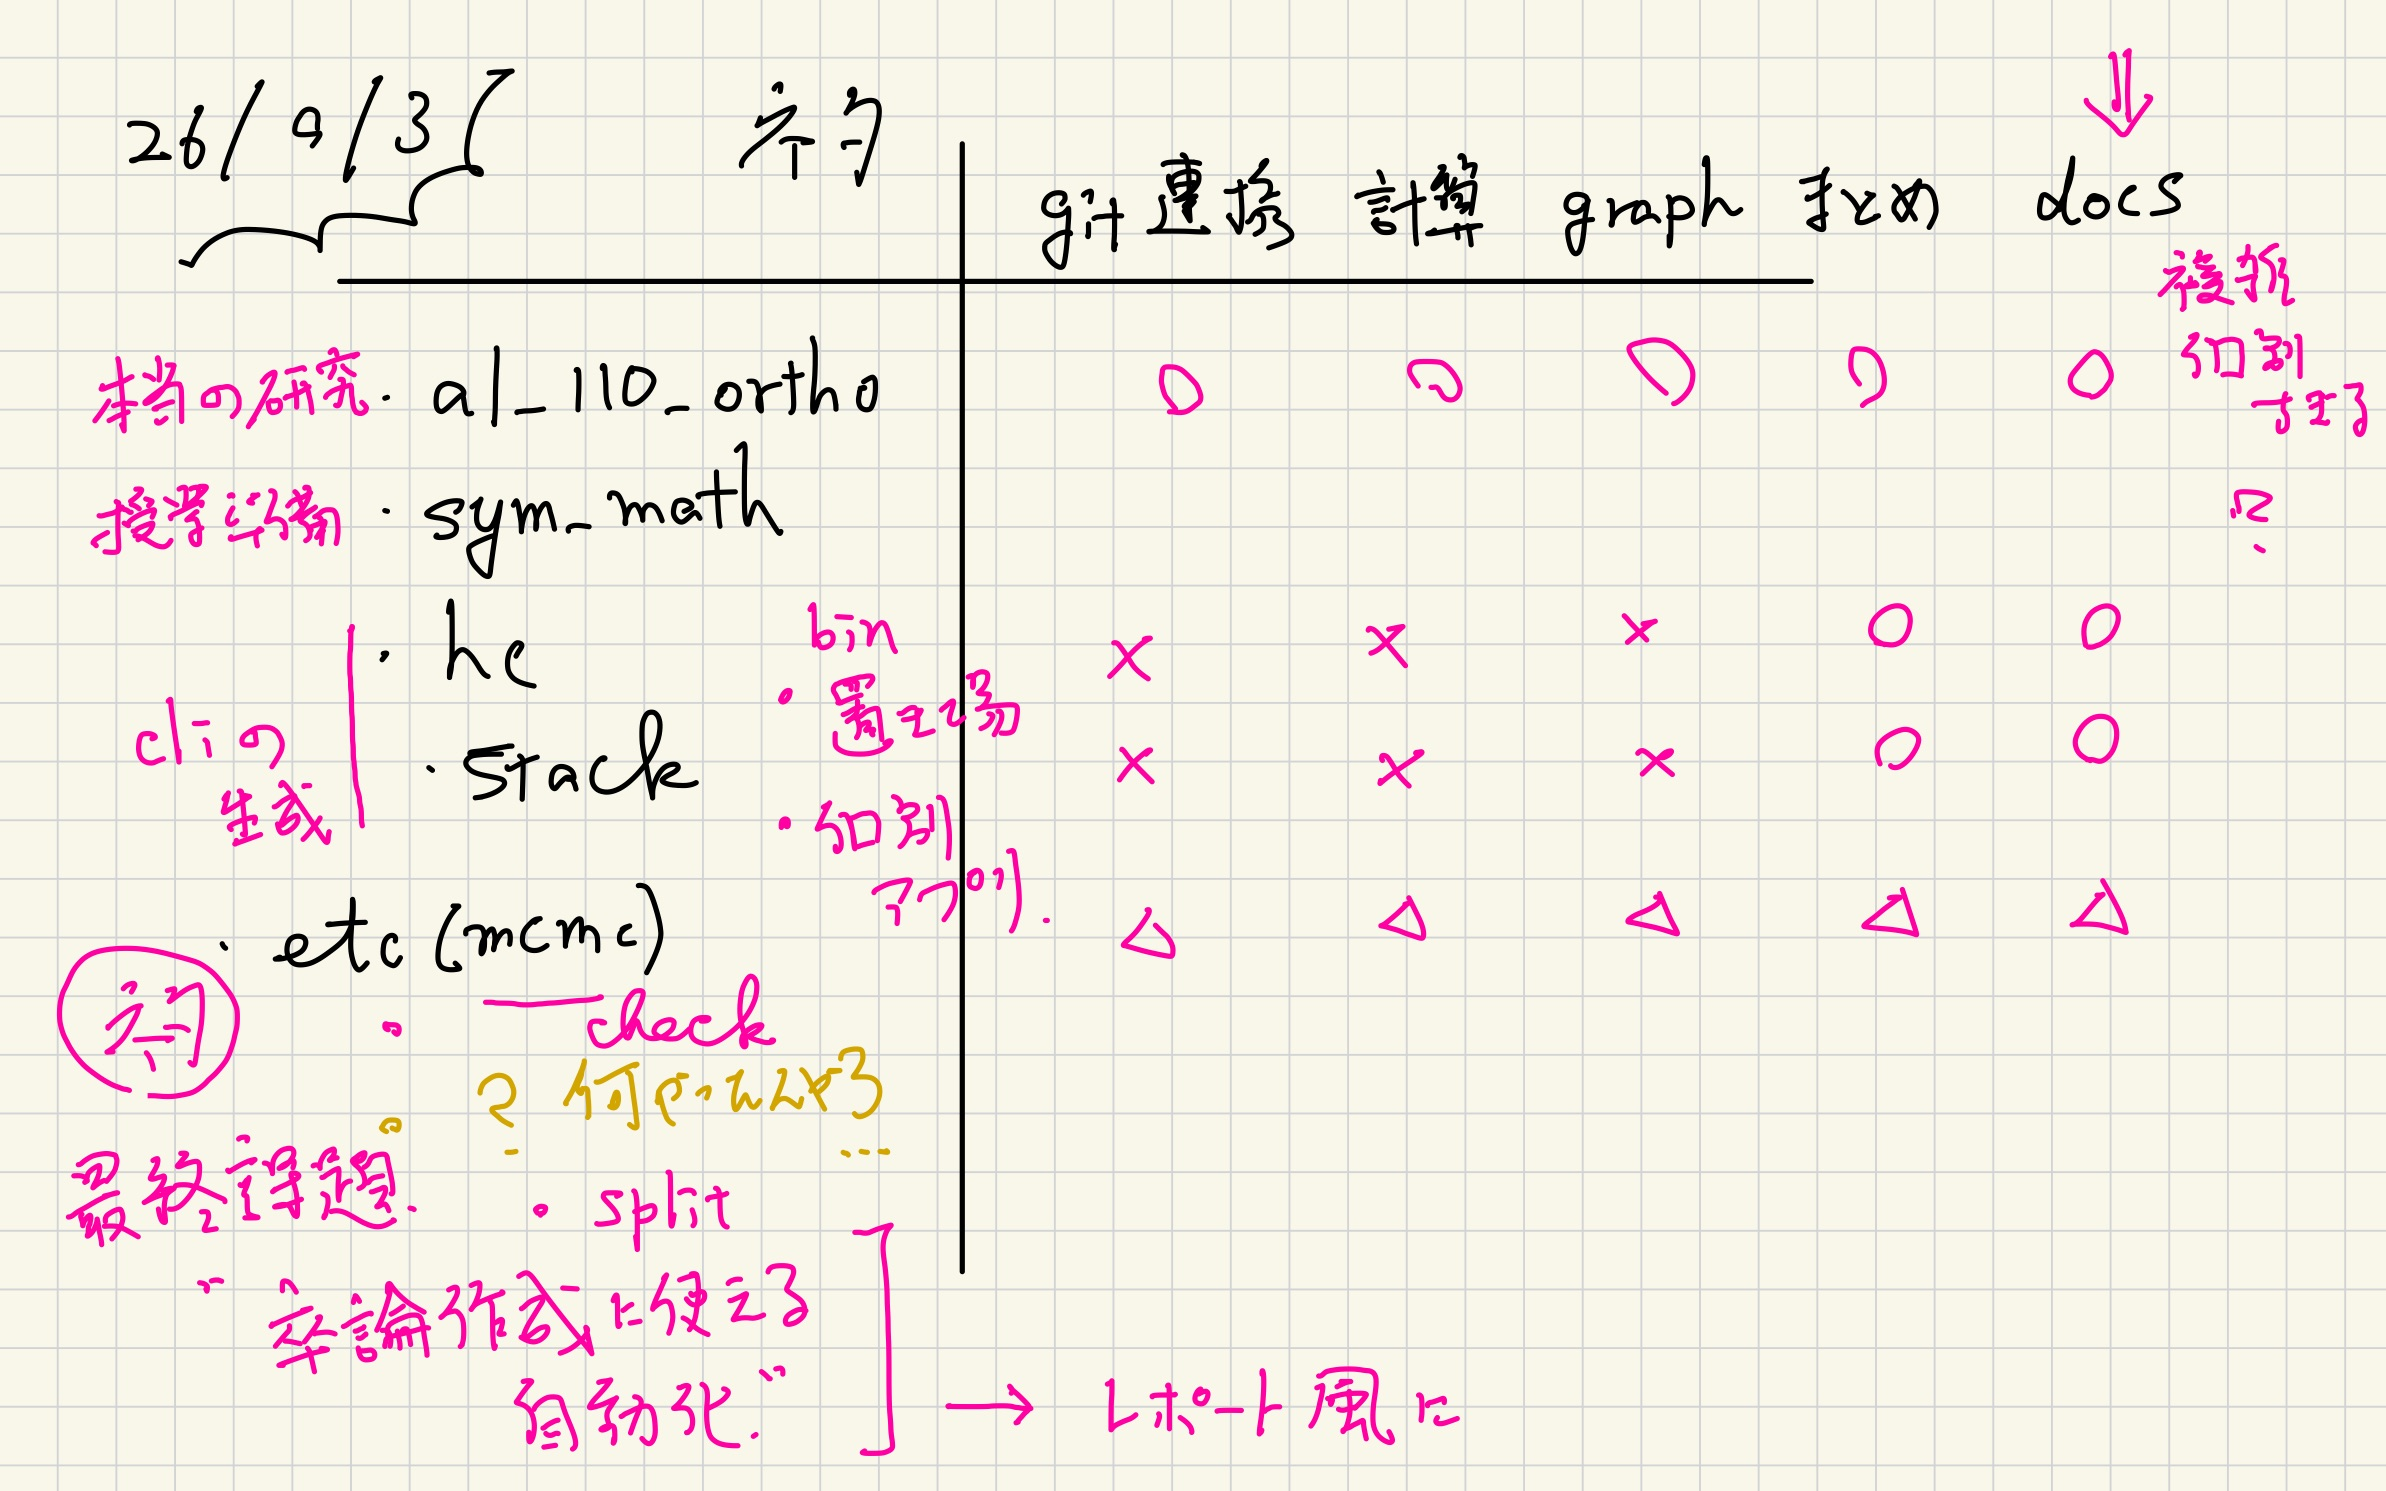
\includegraphics[width=\linewidth]{../d1_mock/figs/prepare_jpgs/hyper_card_system-90.jpg} & 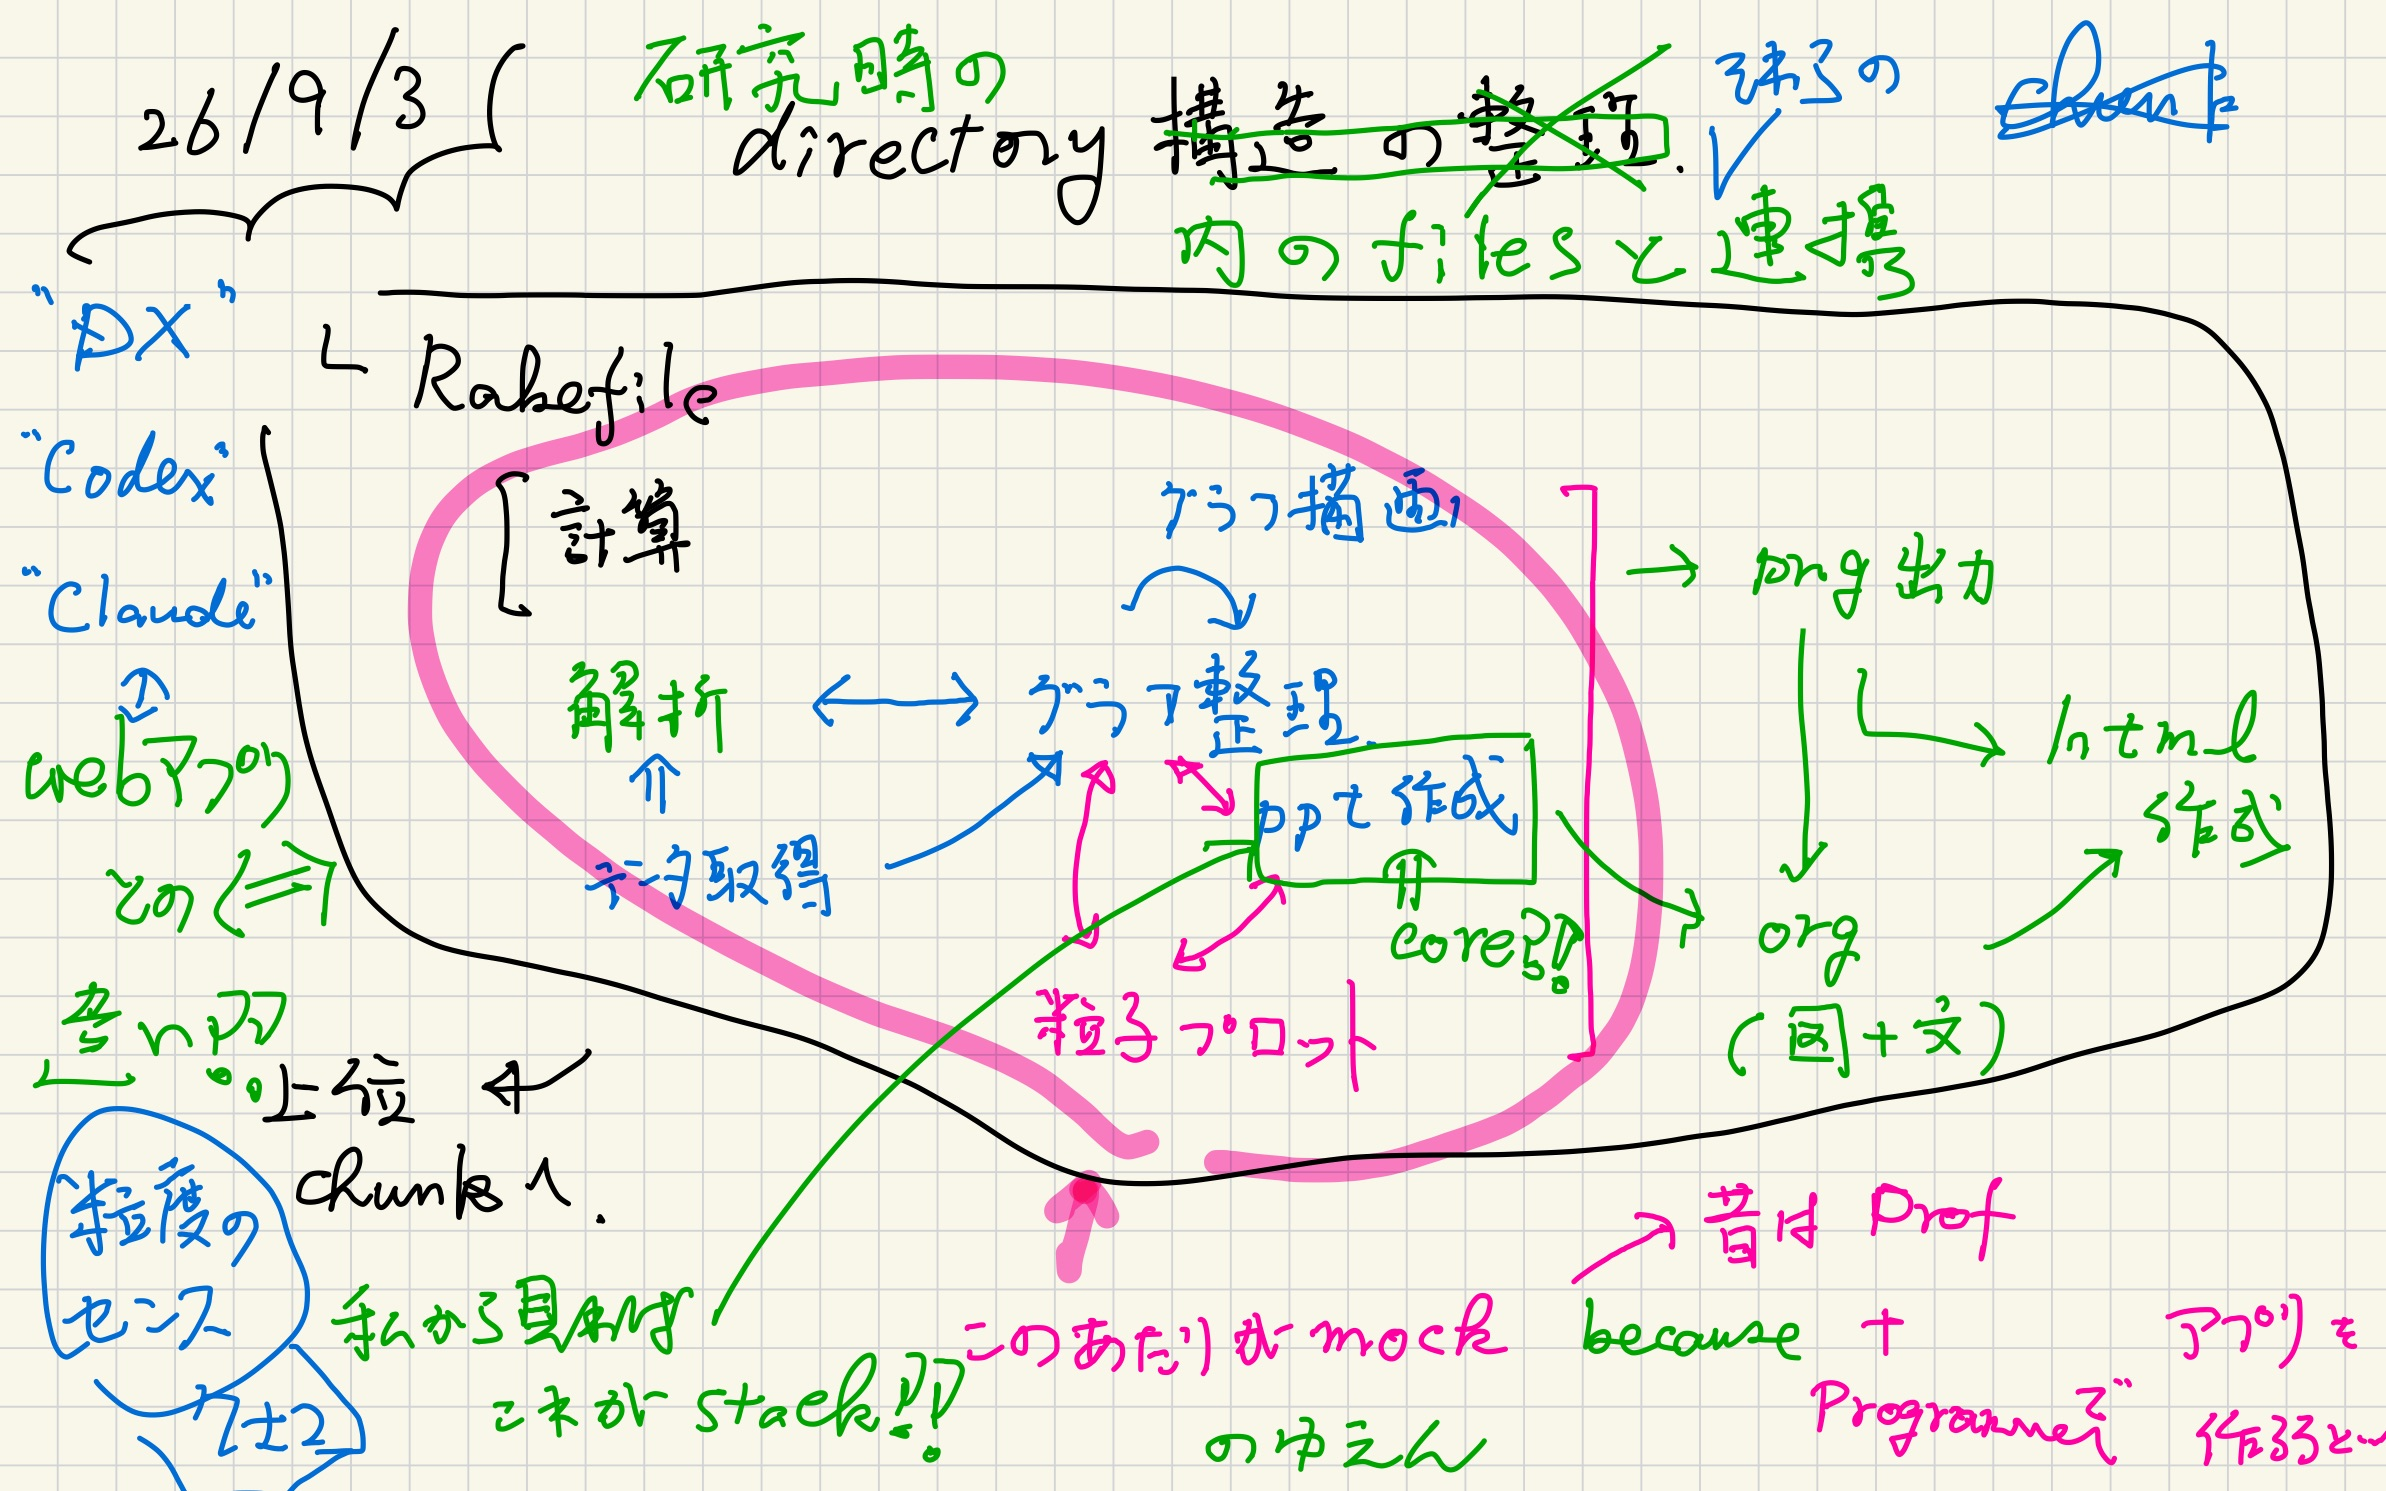
\includegraphics[width=\linewidth]{../d1_mock/figs/prepare_jpgs/hyper_card_system-91.jpg}\\
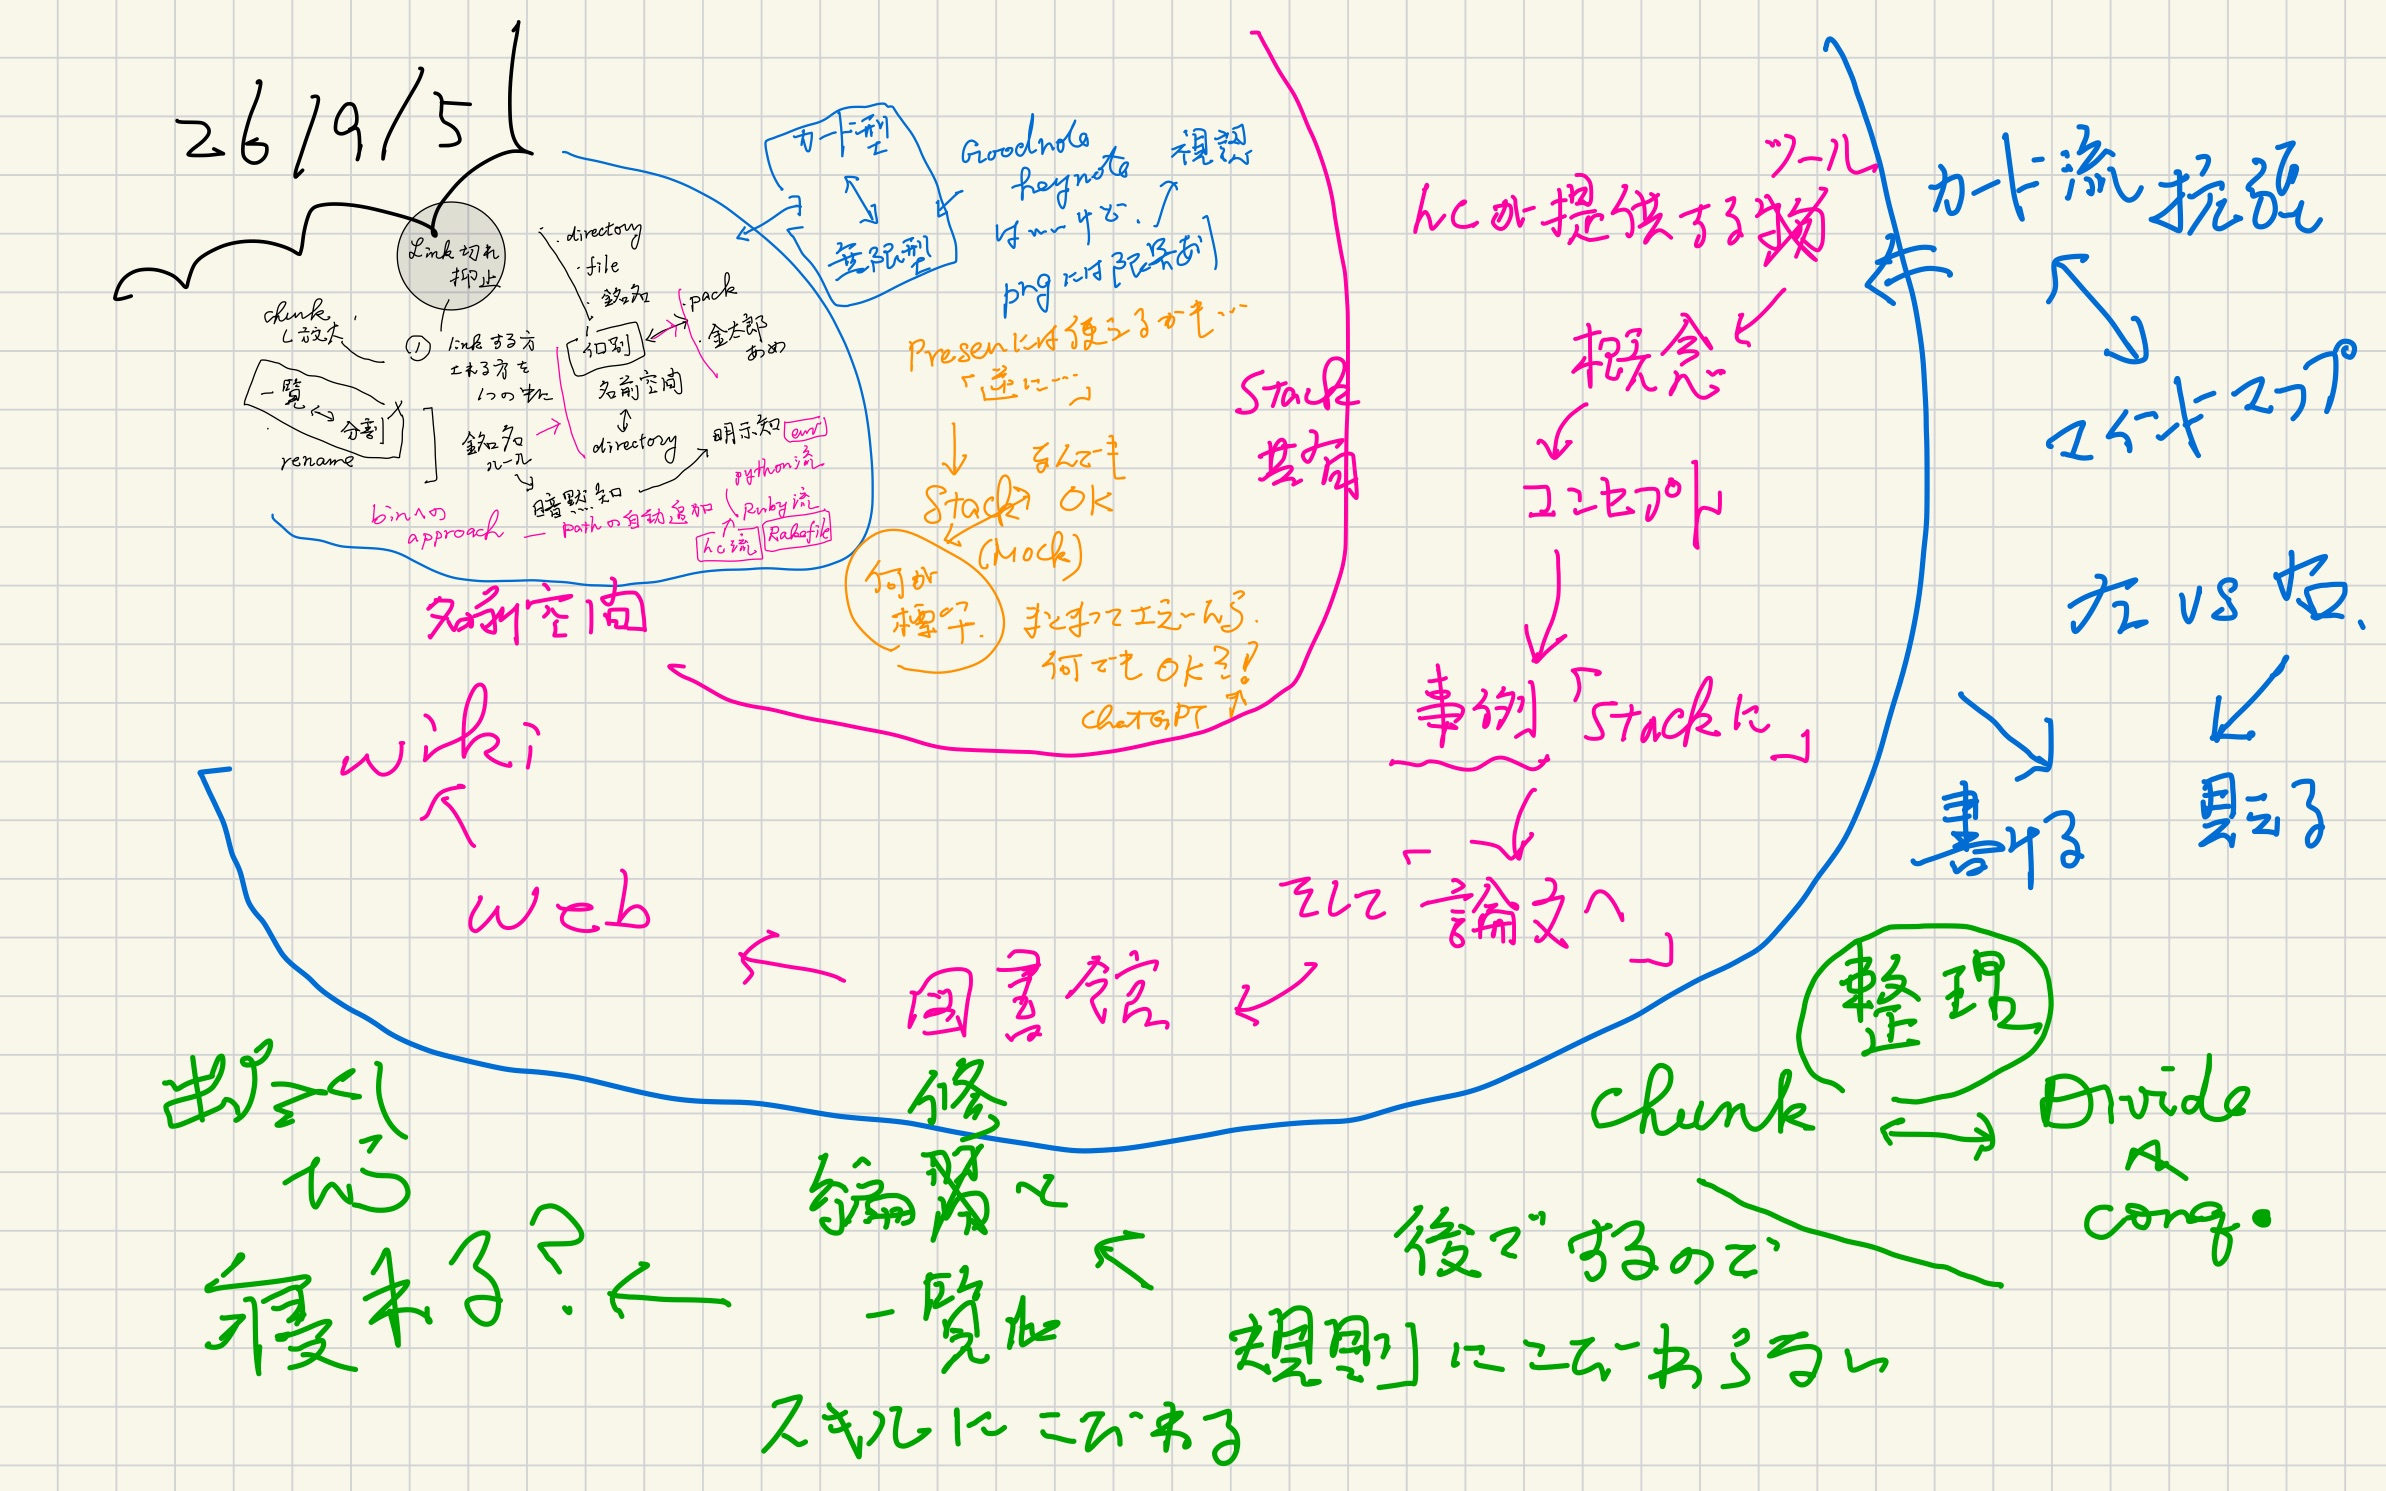
\includegraphics[width=\linewidth]{../d1_mock/figs/prepare_jpgs/hyper_card_system-92.jpg} & 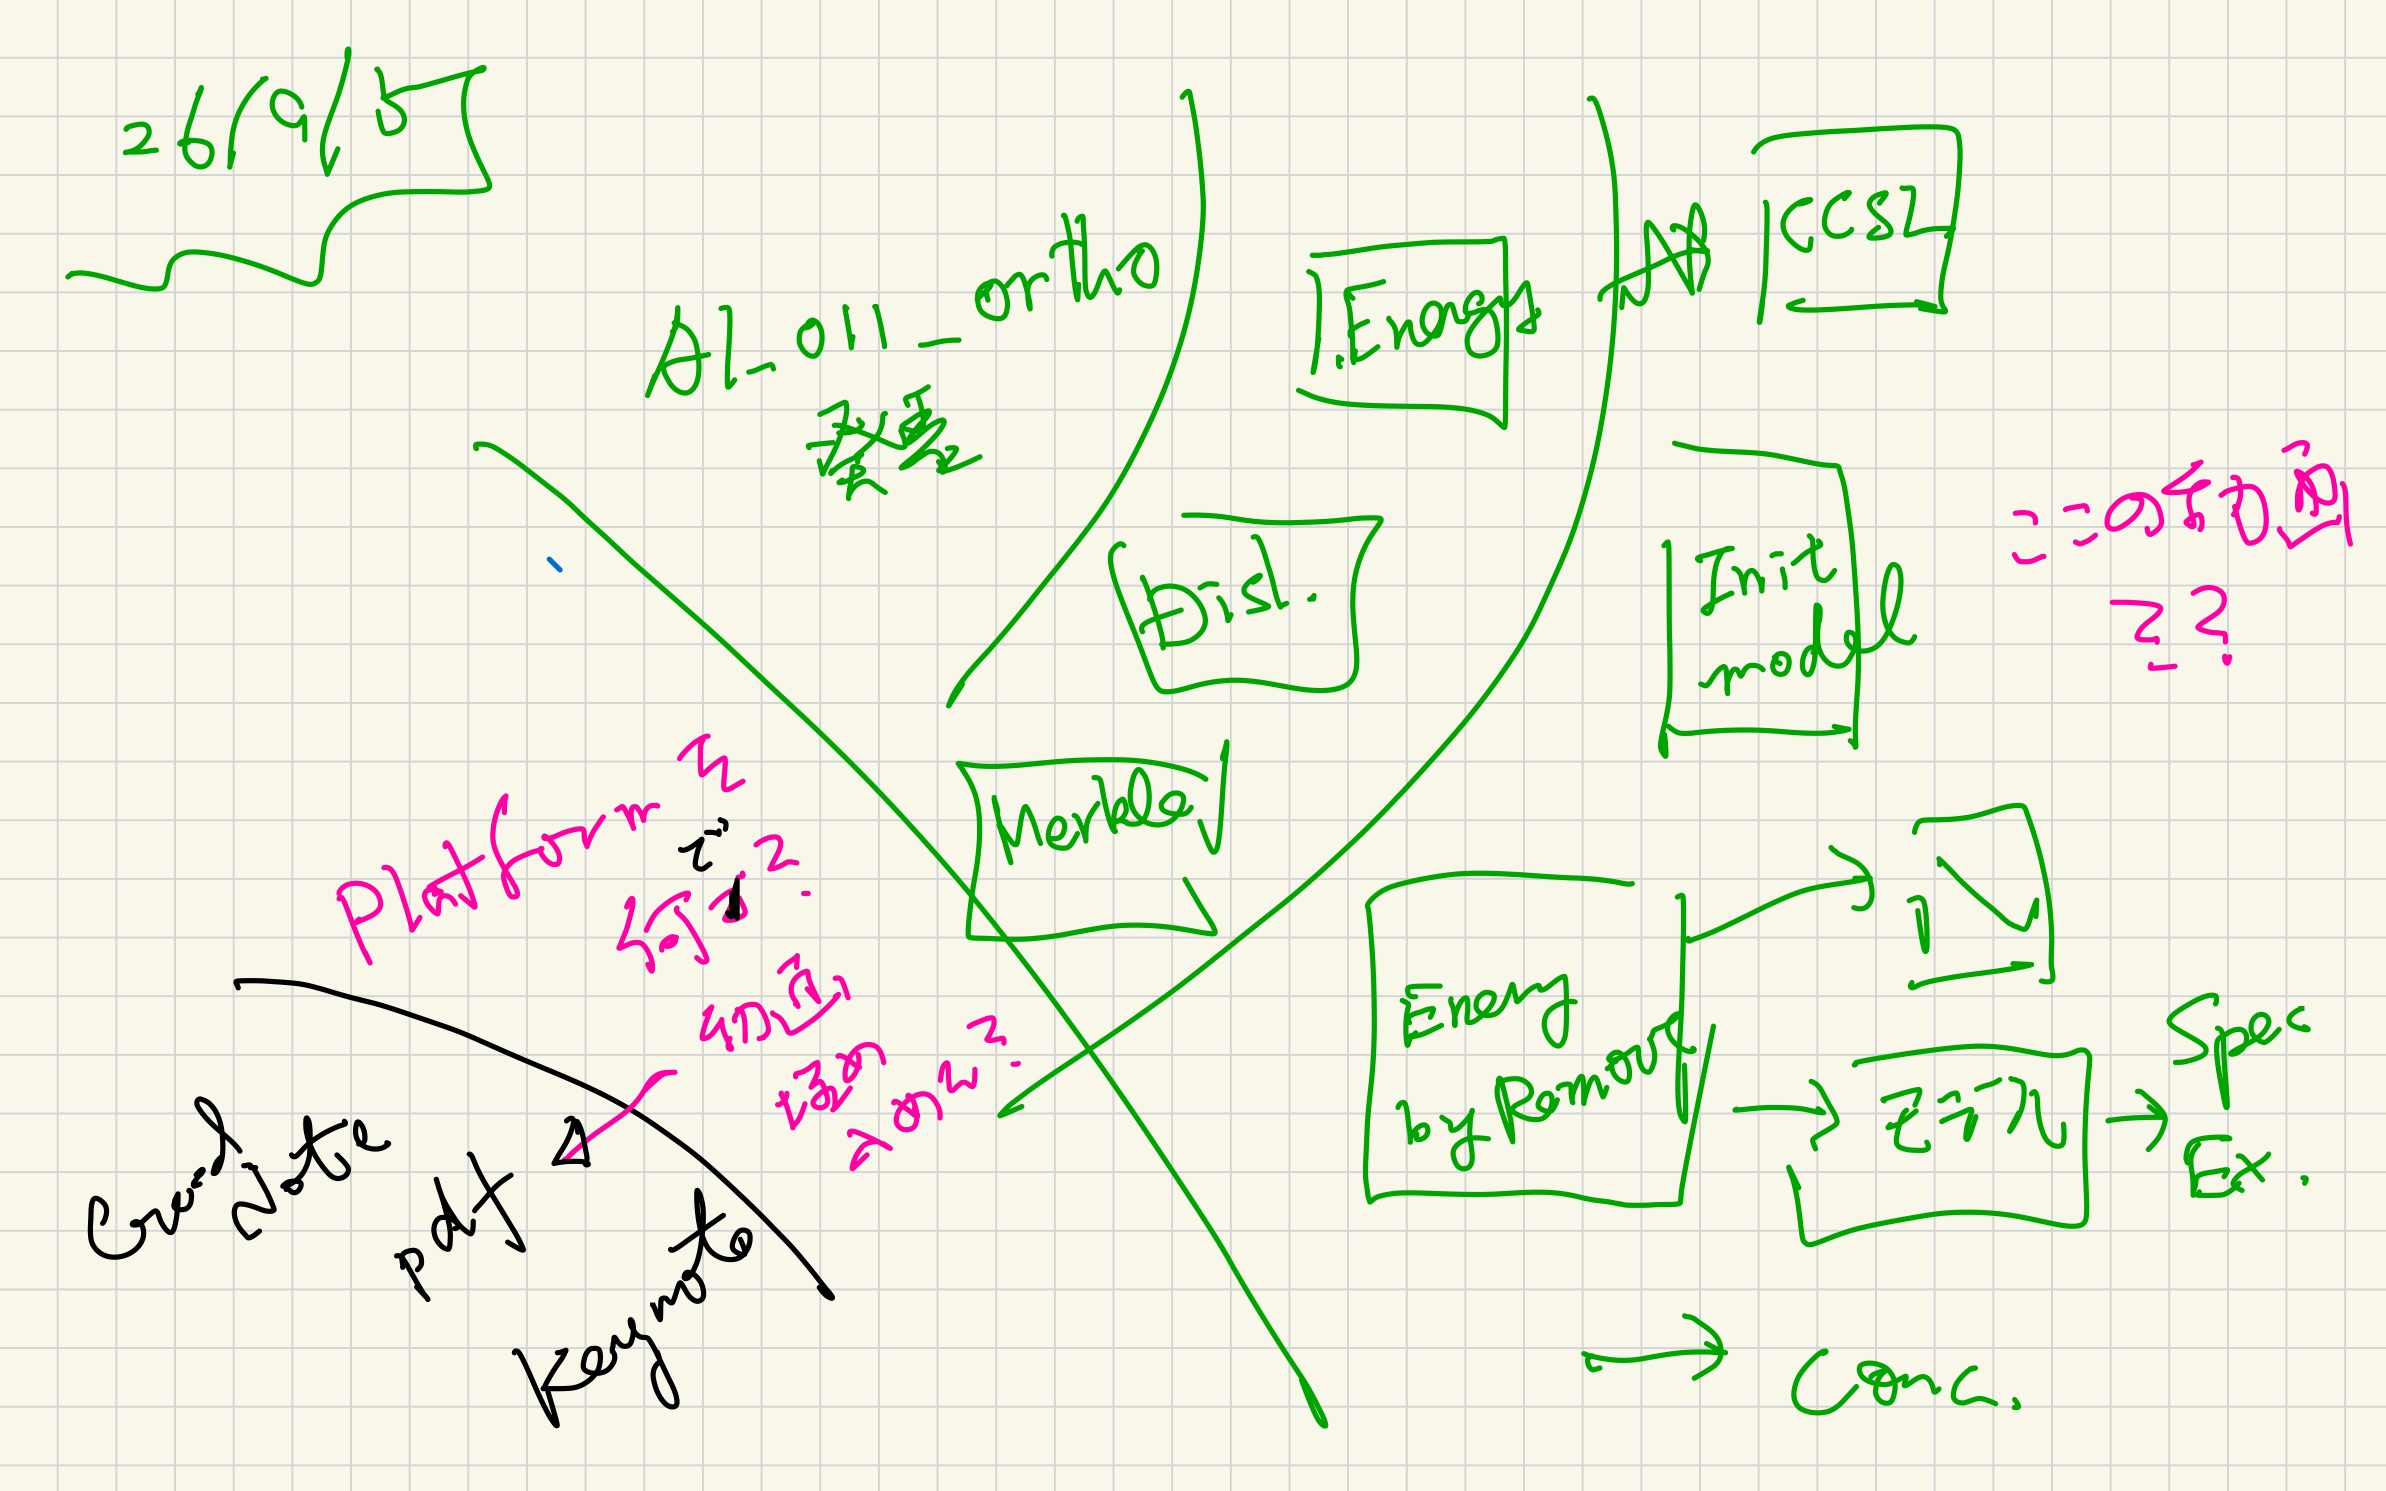
\includegraphics[width=\linewidth]{../d1_mock/figs/prepare_jpgs/hyper_card_system-93.jpg} & 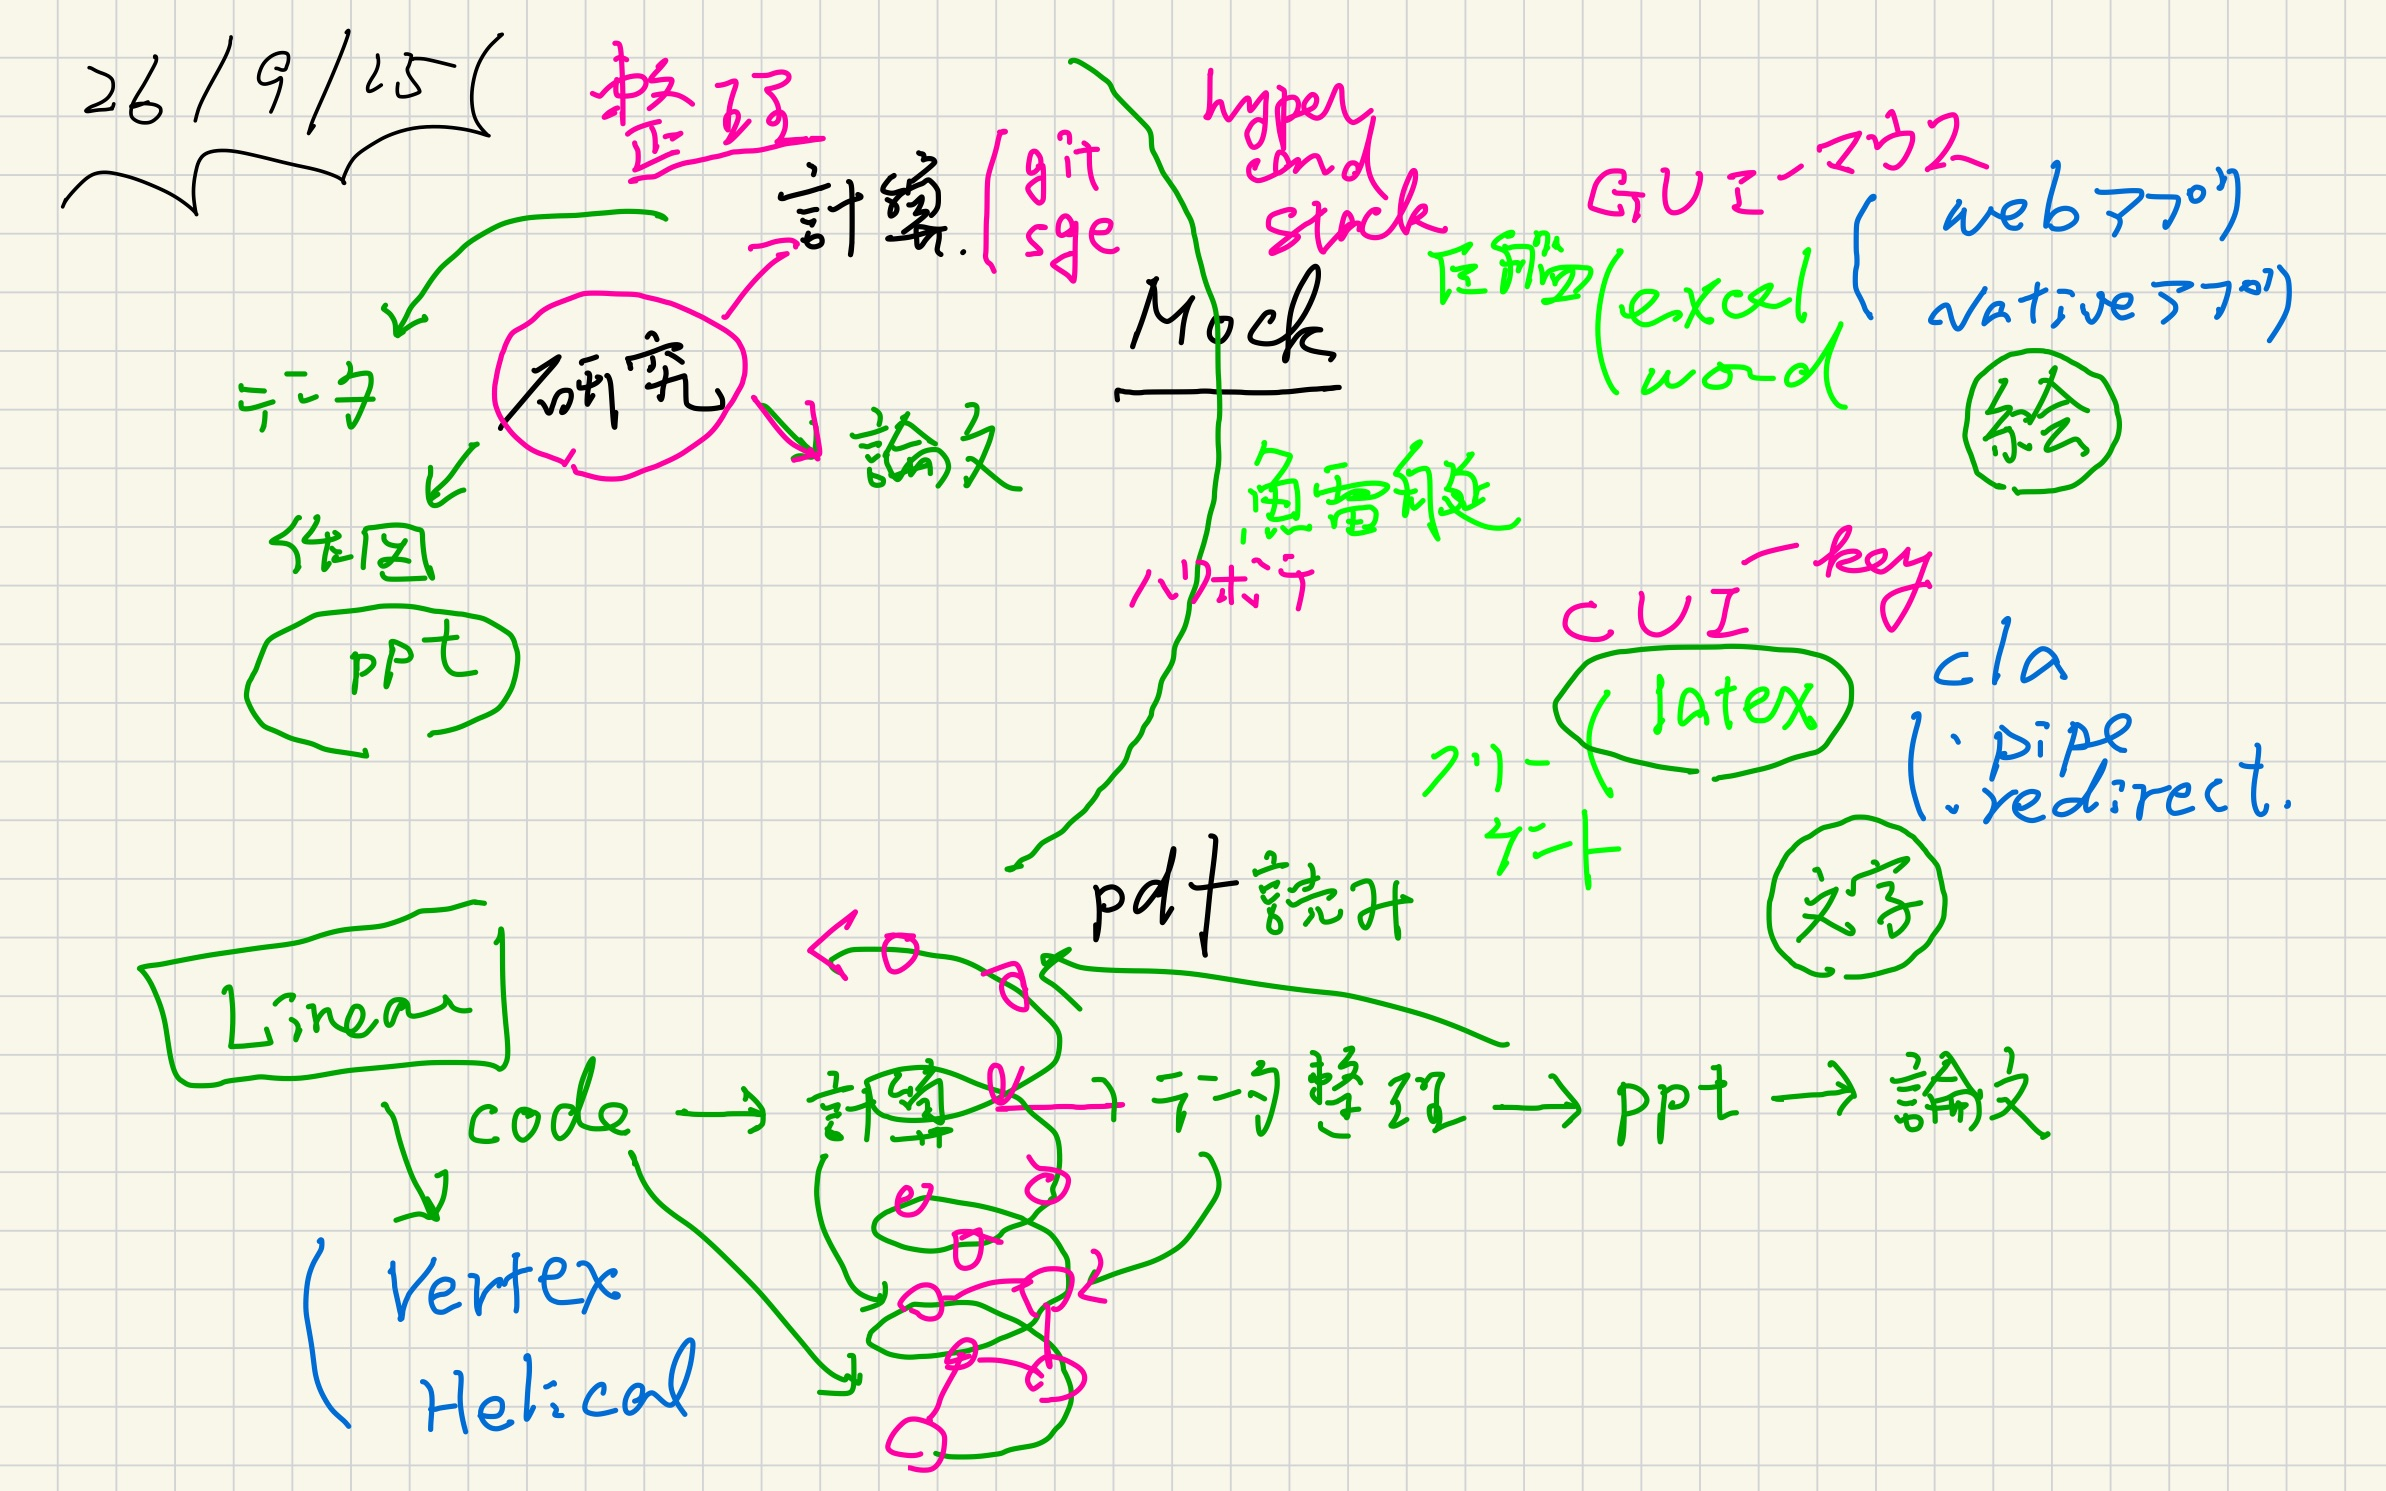
\includegraphics[width=\linewidth]{../d1_mock/figs/prepare_jpgs/hyper_card_system-95.jpg}\\
\end{tabular}
\end{center}
\section{Method}
\label{sec:orga7fc9b1}
\href{../d1\_mock/readme.html}{prev\_button}
\href{../canvas.html}{up\_button}
\href{../d3\_ppt\_pdf/readme.html}{next\_button}
\subsection{chunking, dejavu, HyperCard}
\label{sec:org8eec180}
\begin{center}
\begin{tabular}{p{0.293\linewidth}p{0.293\linewidth}p{0.293\linewidth}}
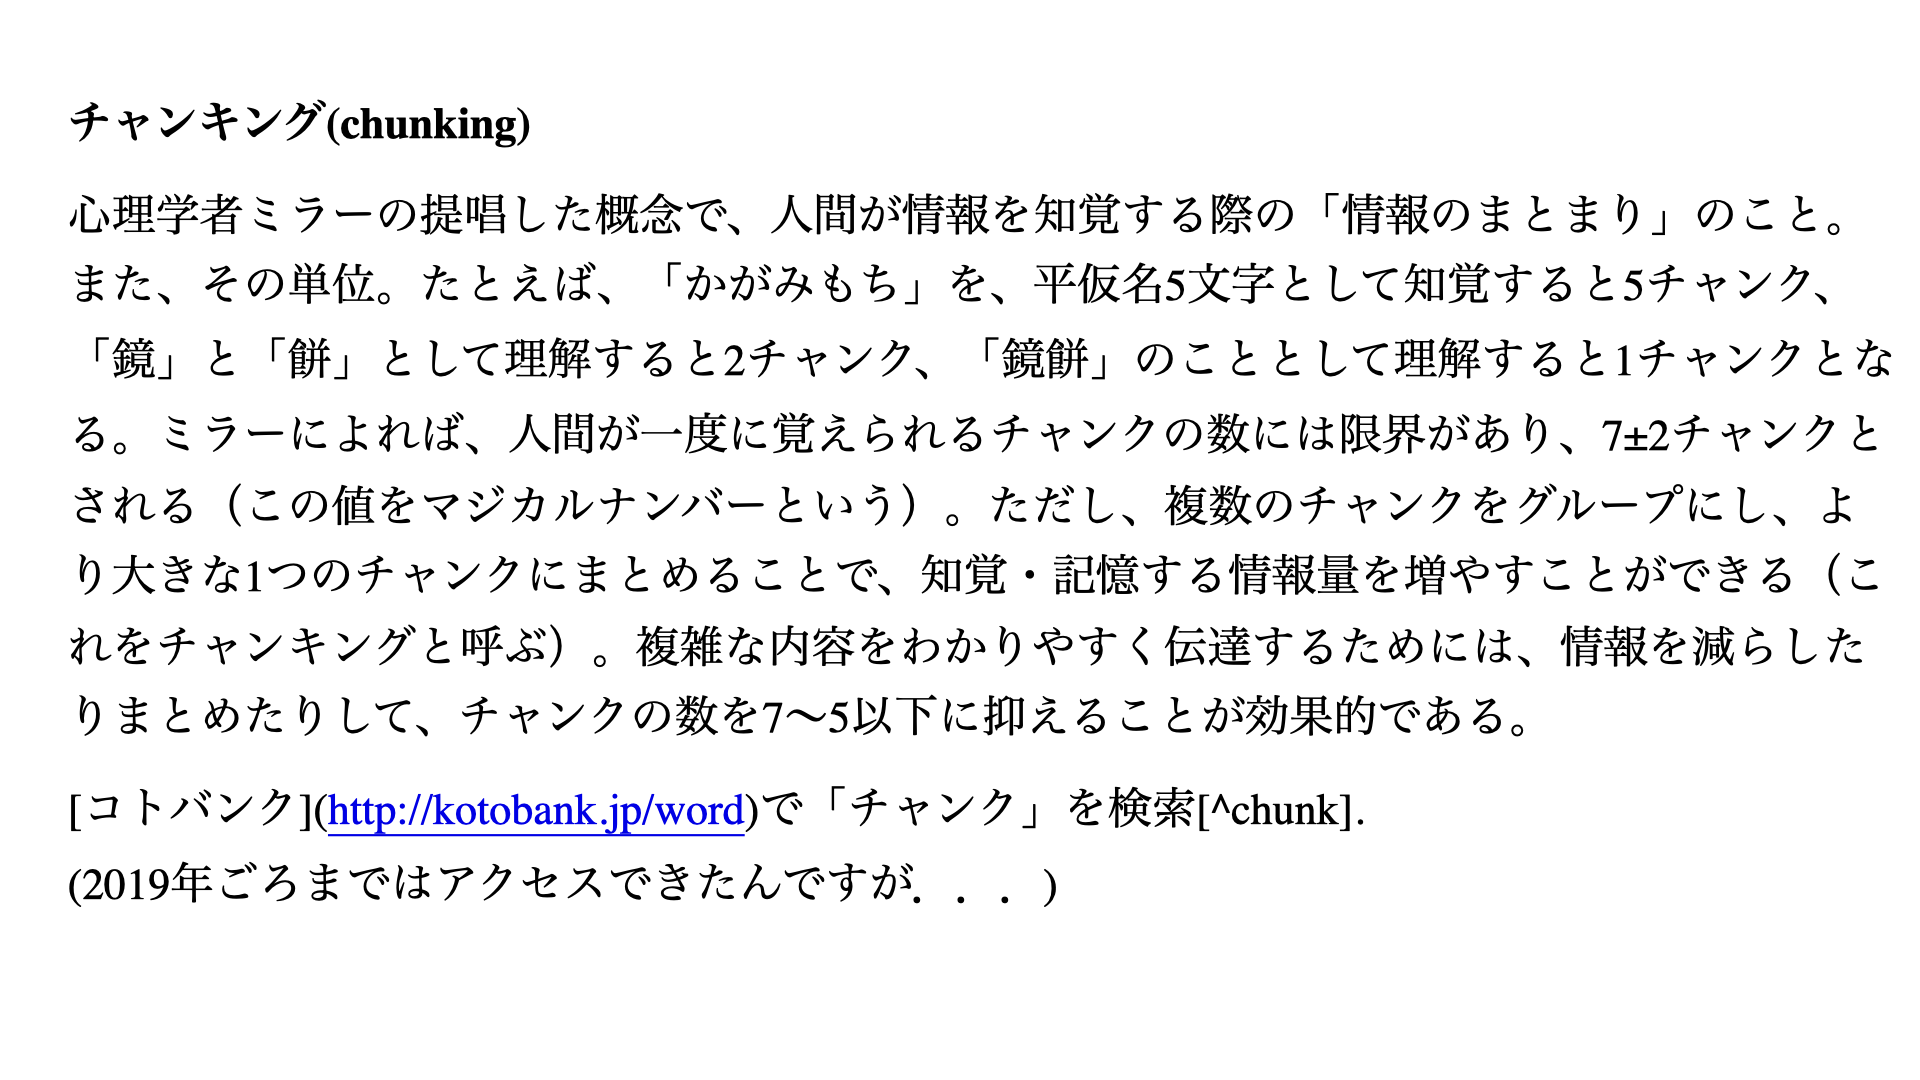
\includegraphics[width=\linewidth]{../d2_divide_chunk/figs/memory.004.png} & 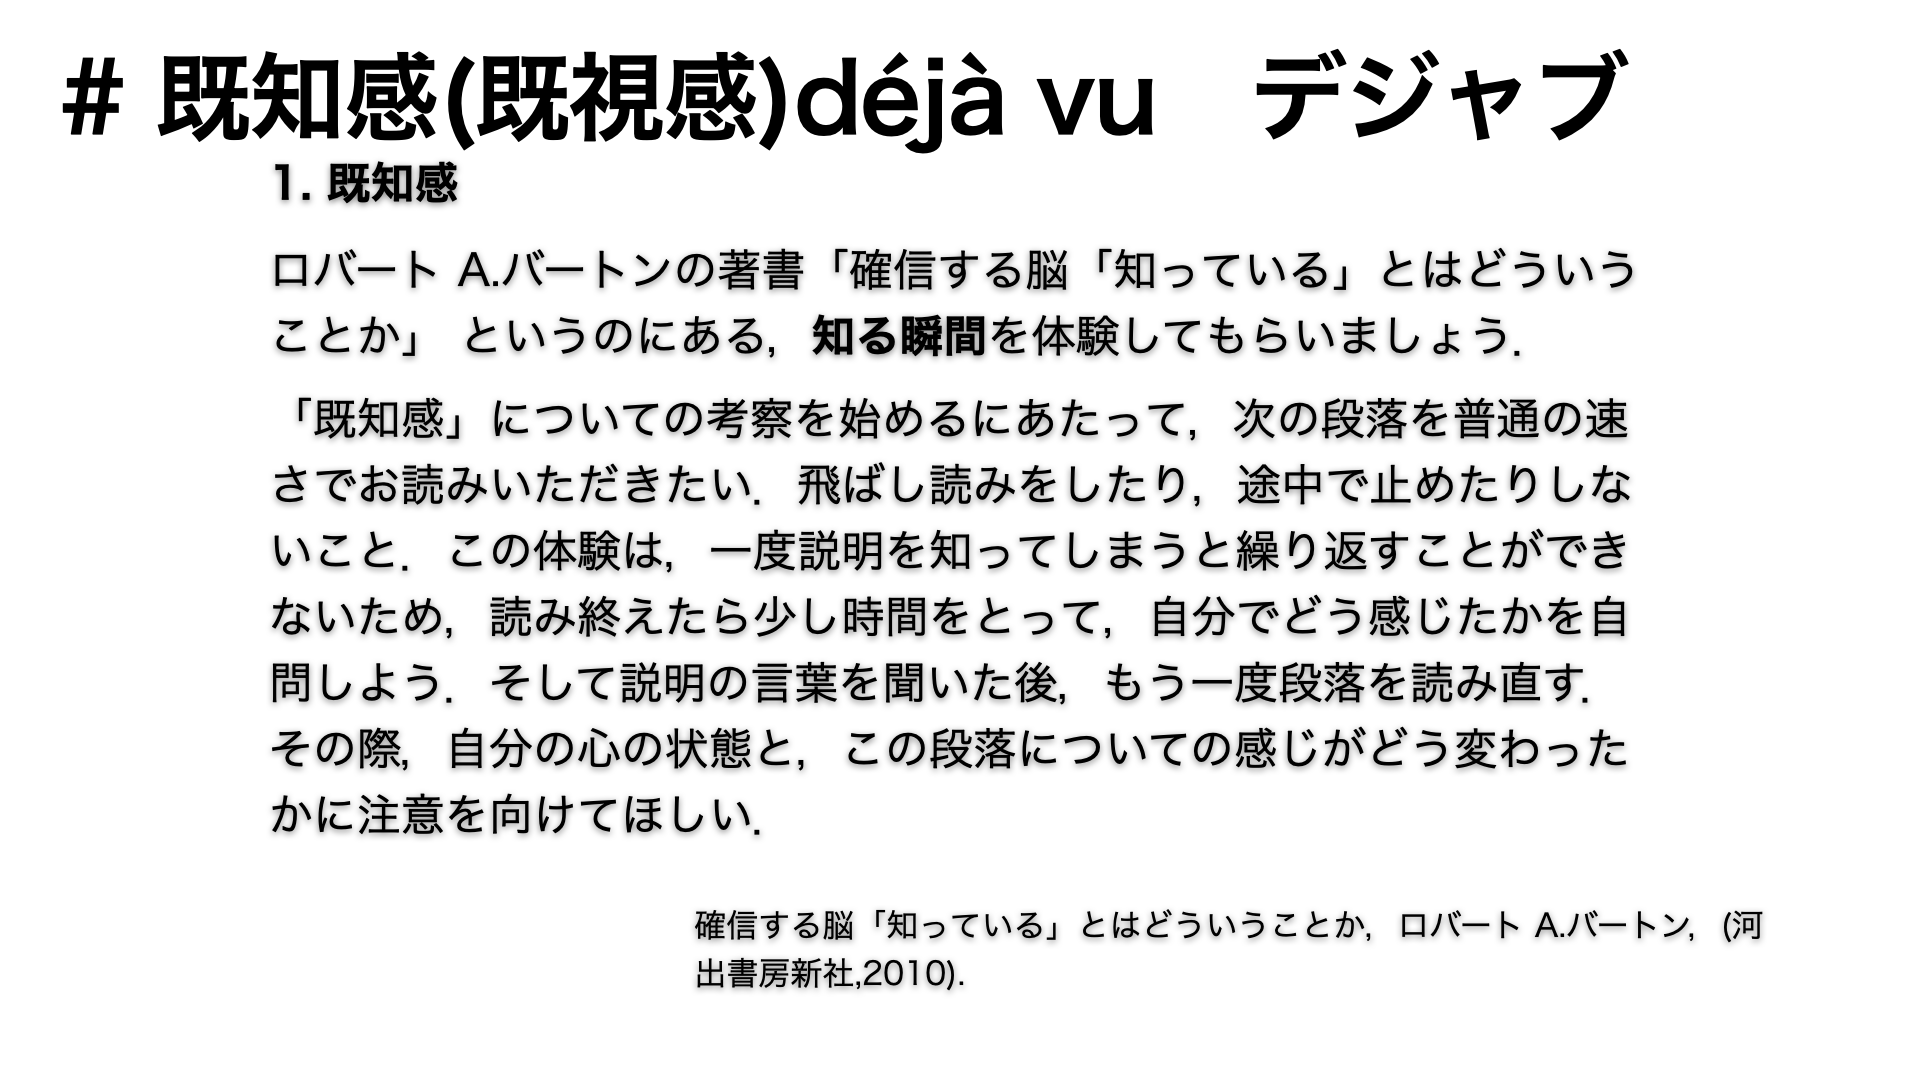
\includegraphics[width=\linewidth]{../d2_divide_chunk/figs/memory.005.png} & 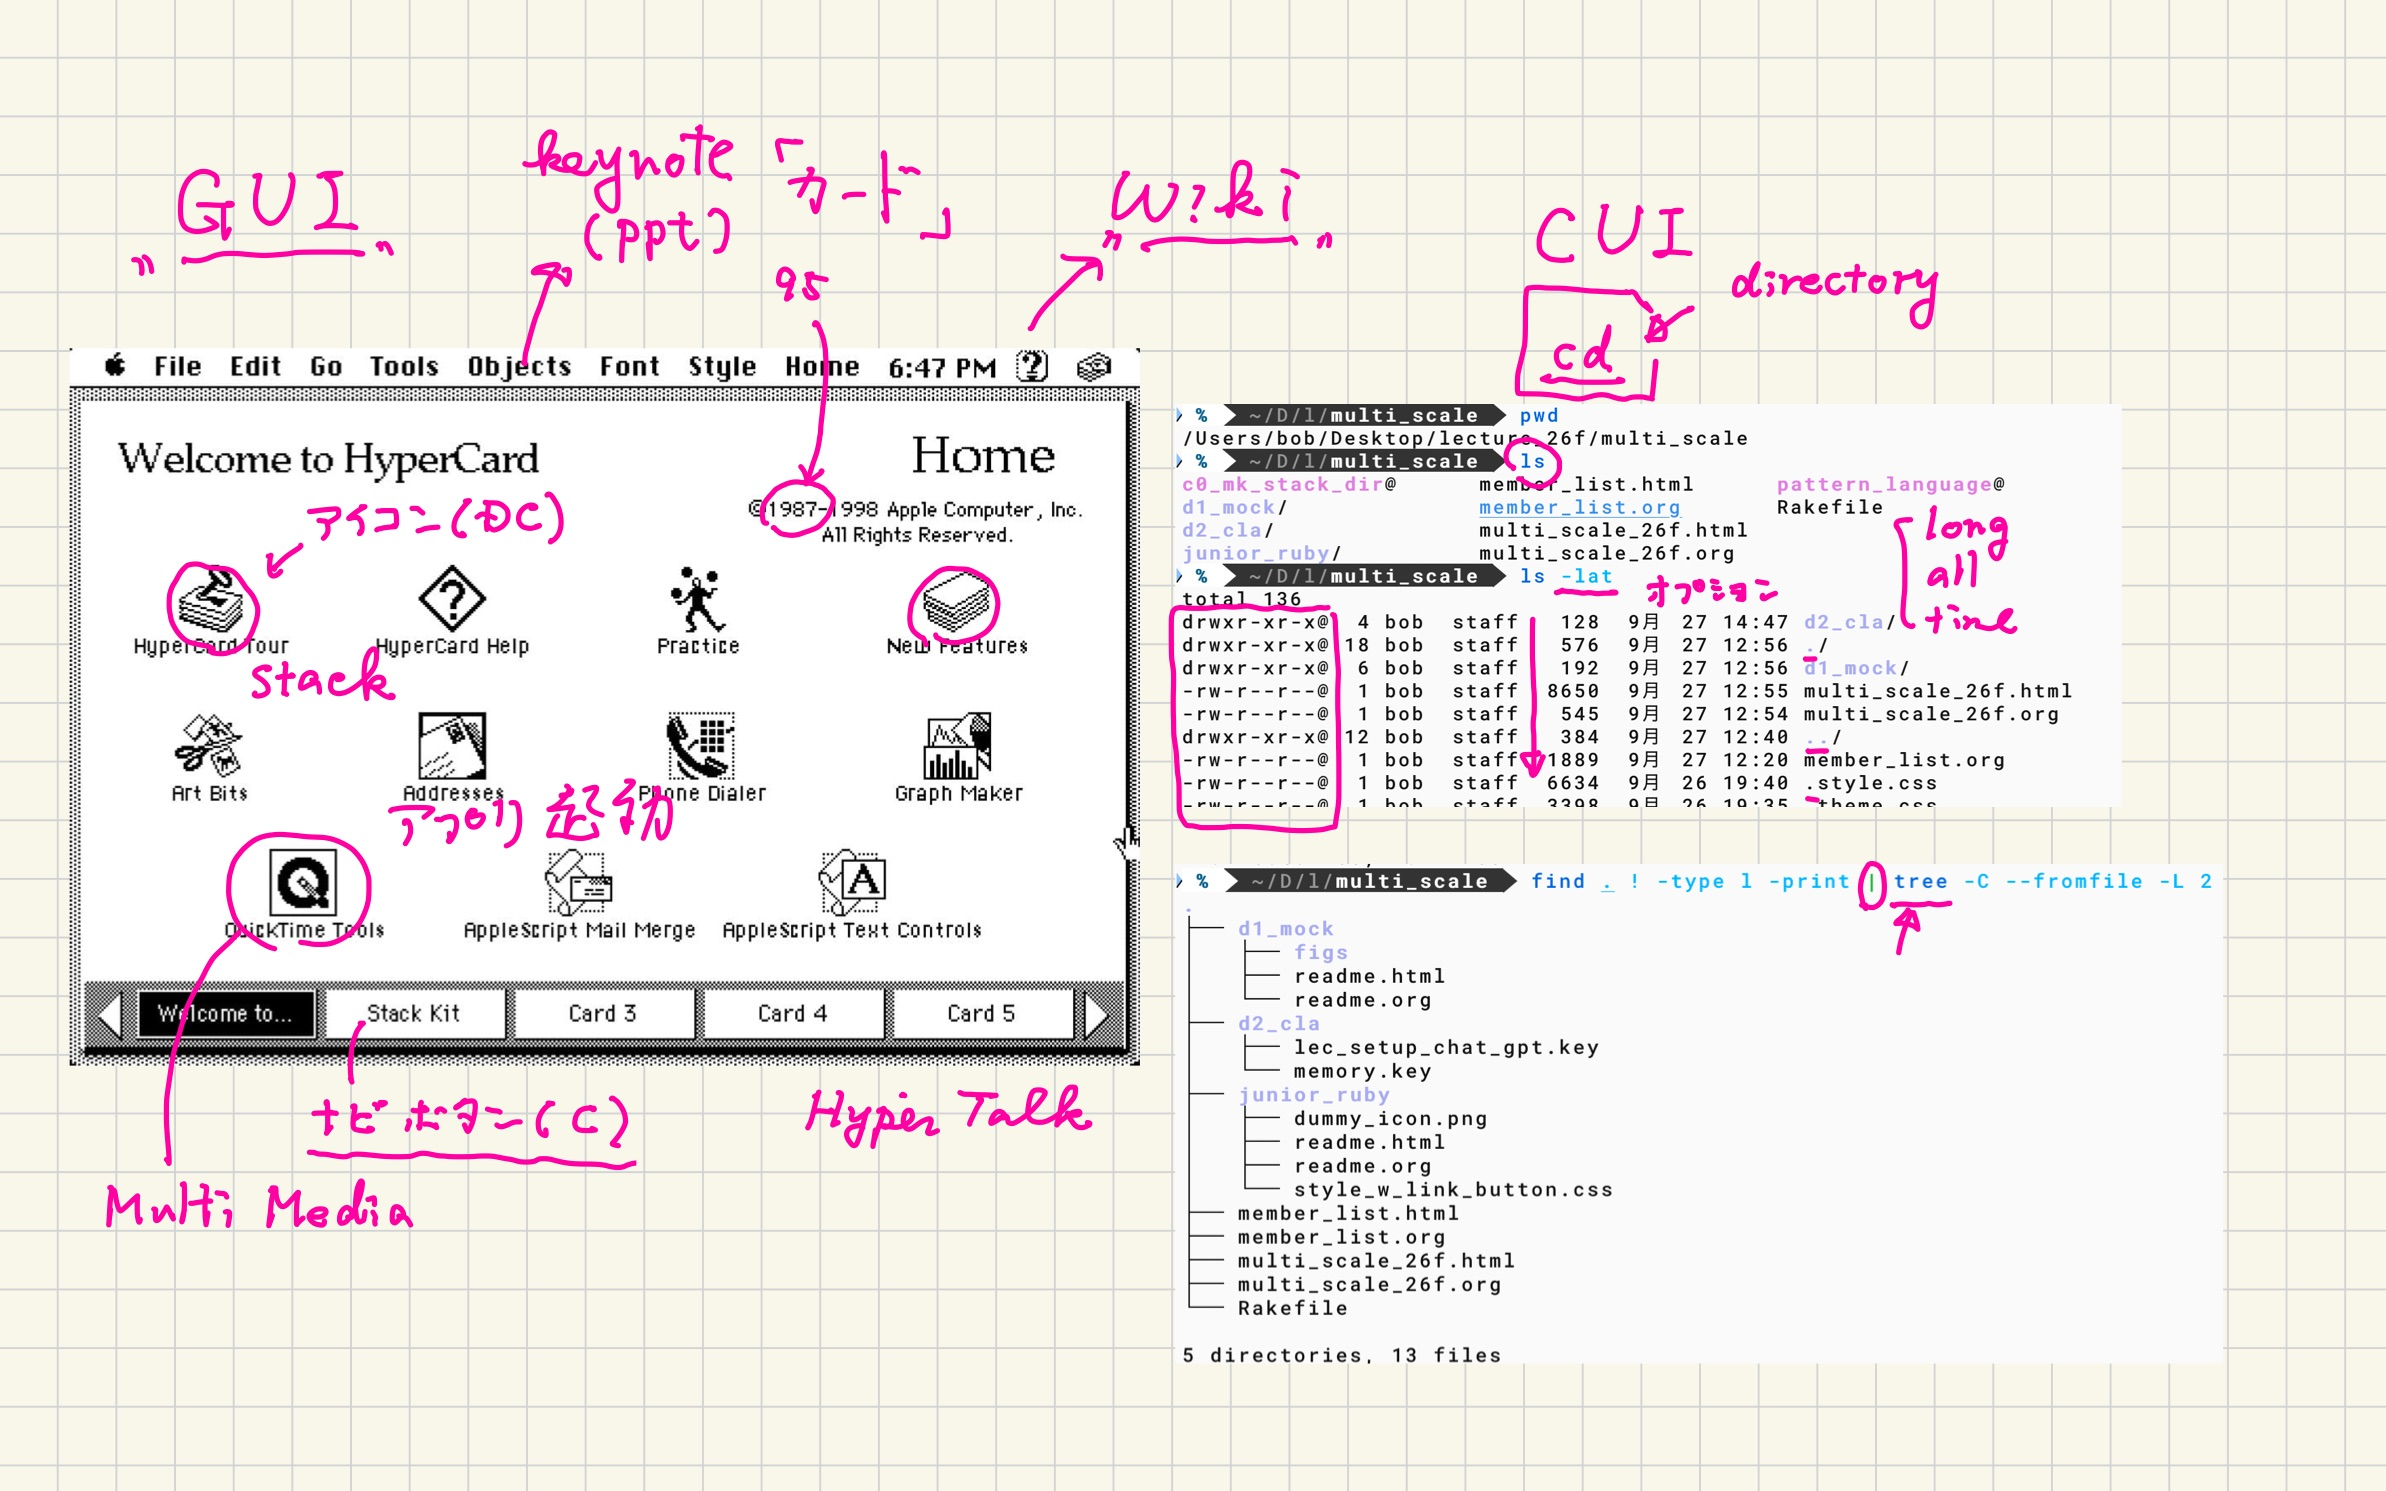
\includegraphics[width=\linewidth]{../d2_divide_chunk/figs/multi_scale_26f-10.jpg}\\
\end{tabular}
\end{center}

Mock-Upの基本になる考え方が
chunkingとdeja vuです．
chunkingはまとまった知識を覚える人間の
癖を心理学者が解き明かした知恵です．
それをまとめる時にはコトバでもって
概念としてまとめます．

これは卒業研究の本質に深く根ざしています．
それらの知識をまとめたのが次の文章です．
\begin{itemize}
\item \url{../d3\_stack/hyper\_card\_philosophy\_w\_gemini.org}
\end{itemize}
\subsection{preparation notes}
\label{sec:org54fddb8}
\begin{center}
\begin{tabular}{p{0.293\linewidth}p{0.293\linewidth}p{0.293\linewidth}}
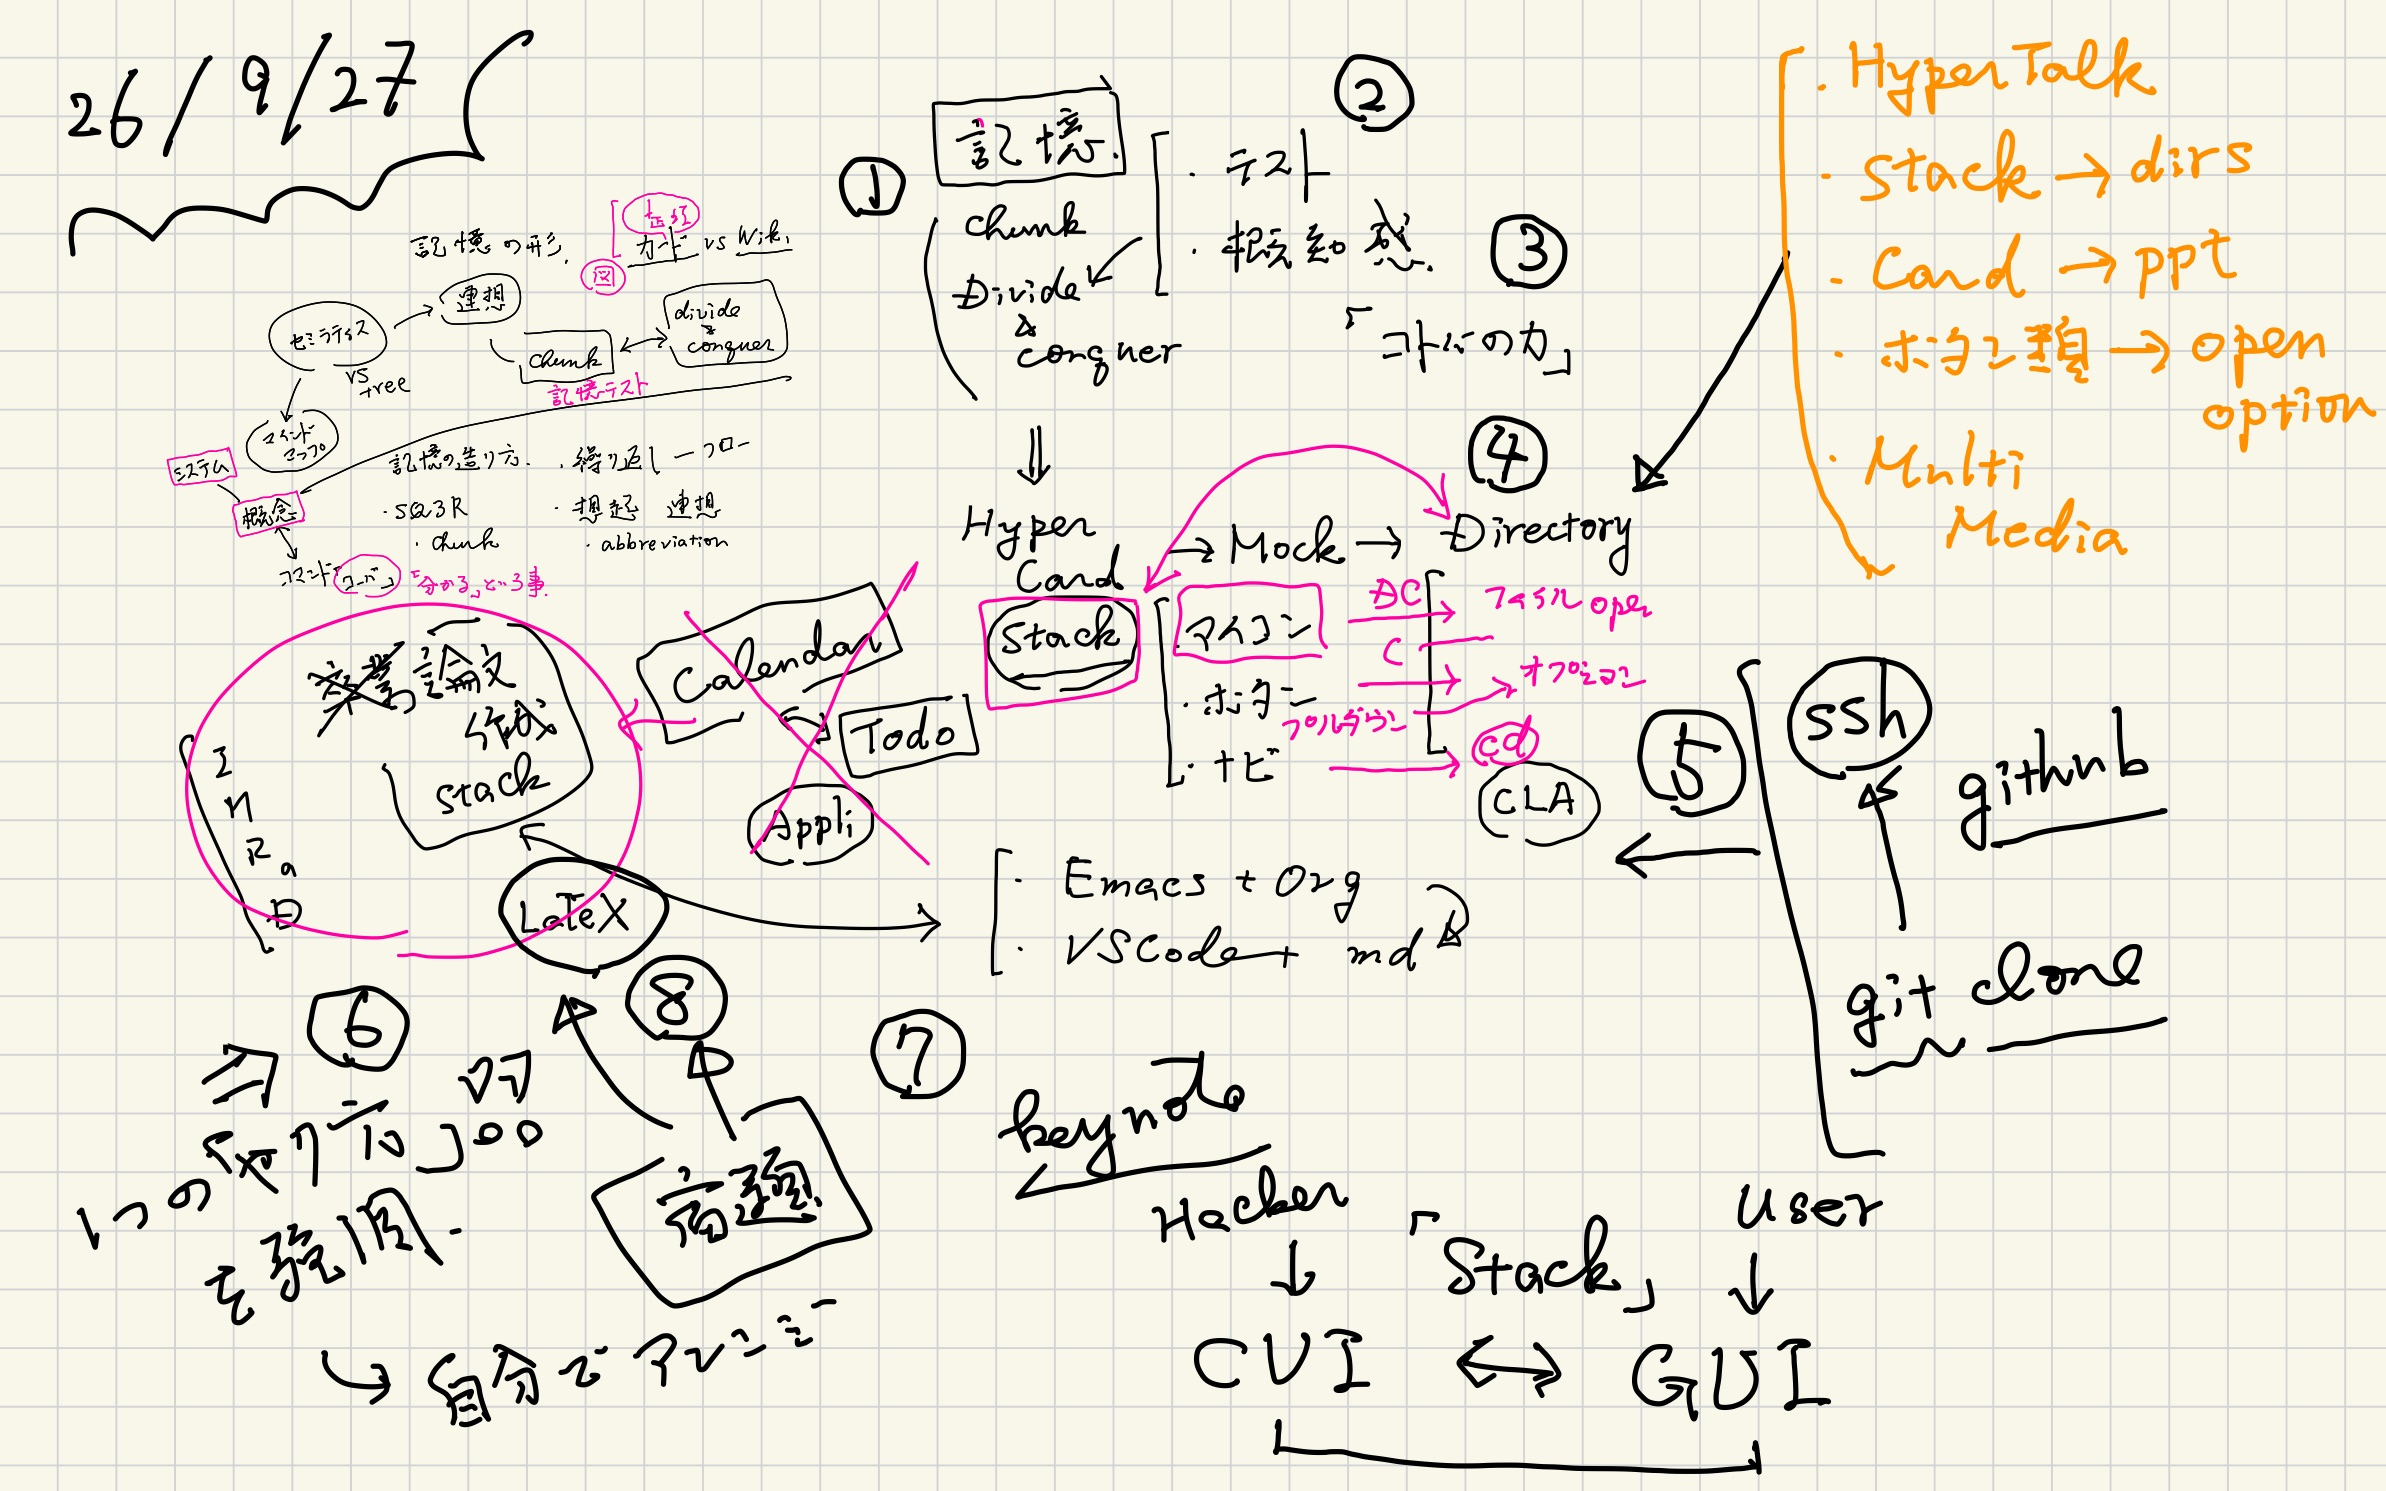
\includegraphics[width=\linewidth]{../d2_divide_chunk/figs/multi_scale_26f-8.jpg} & 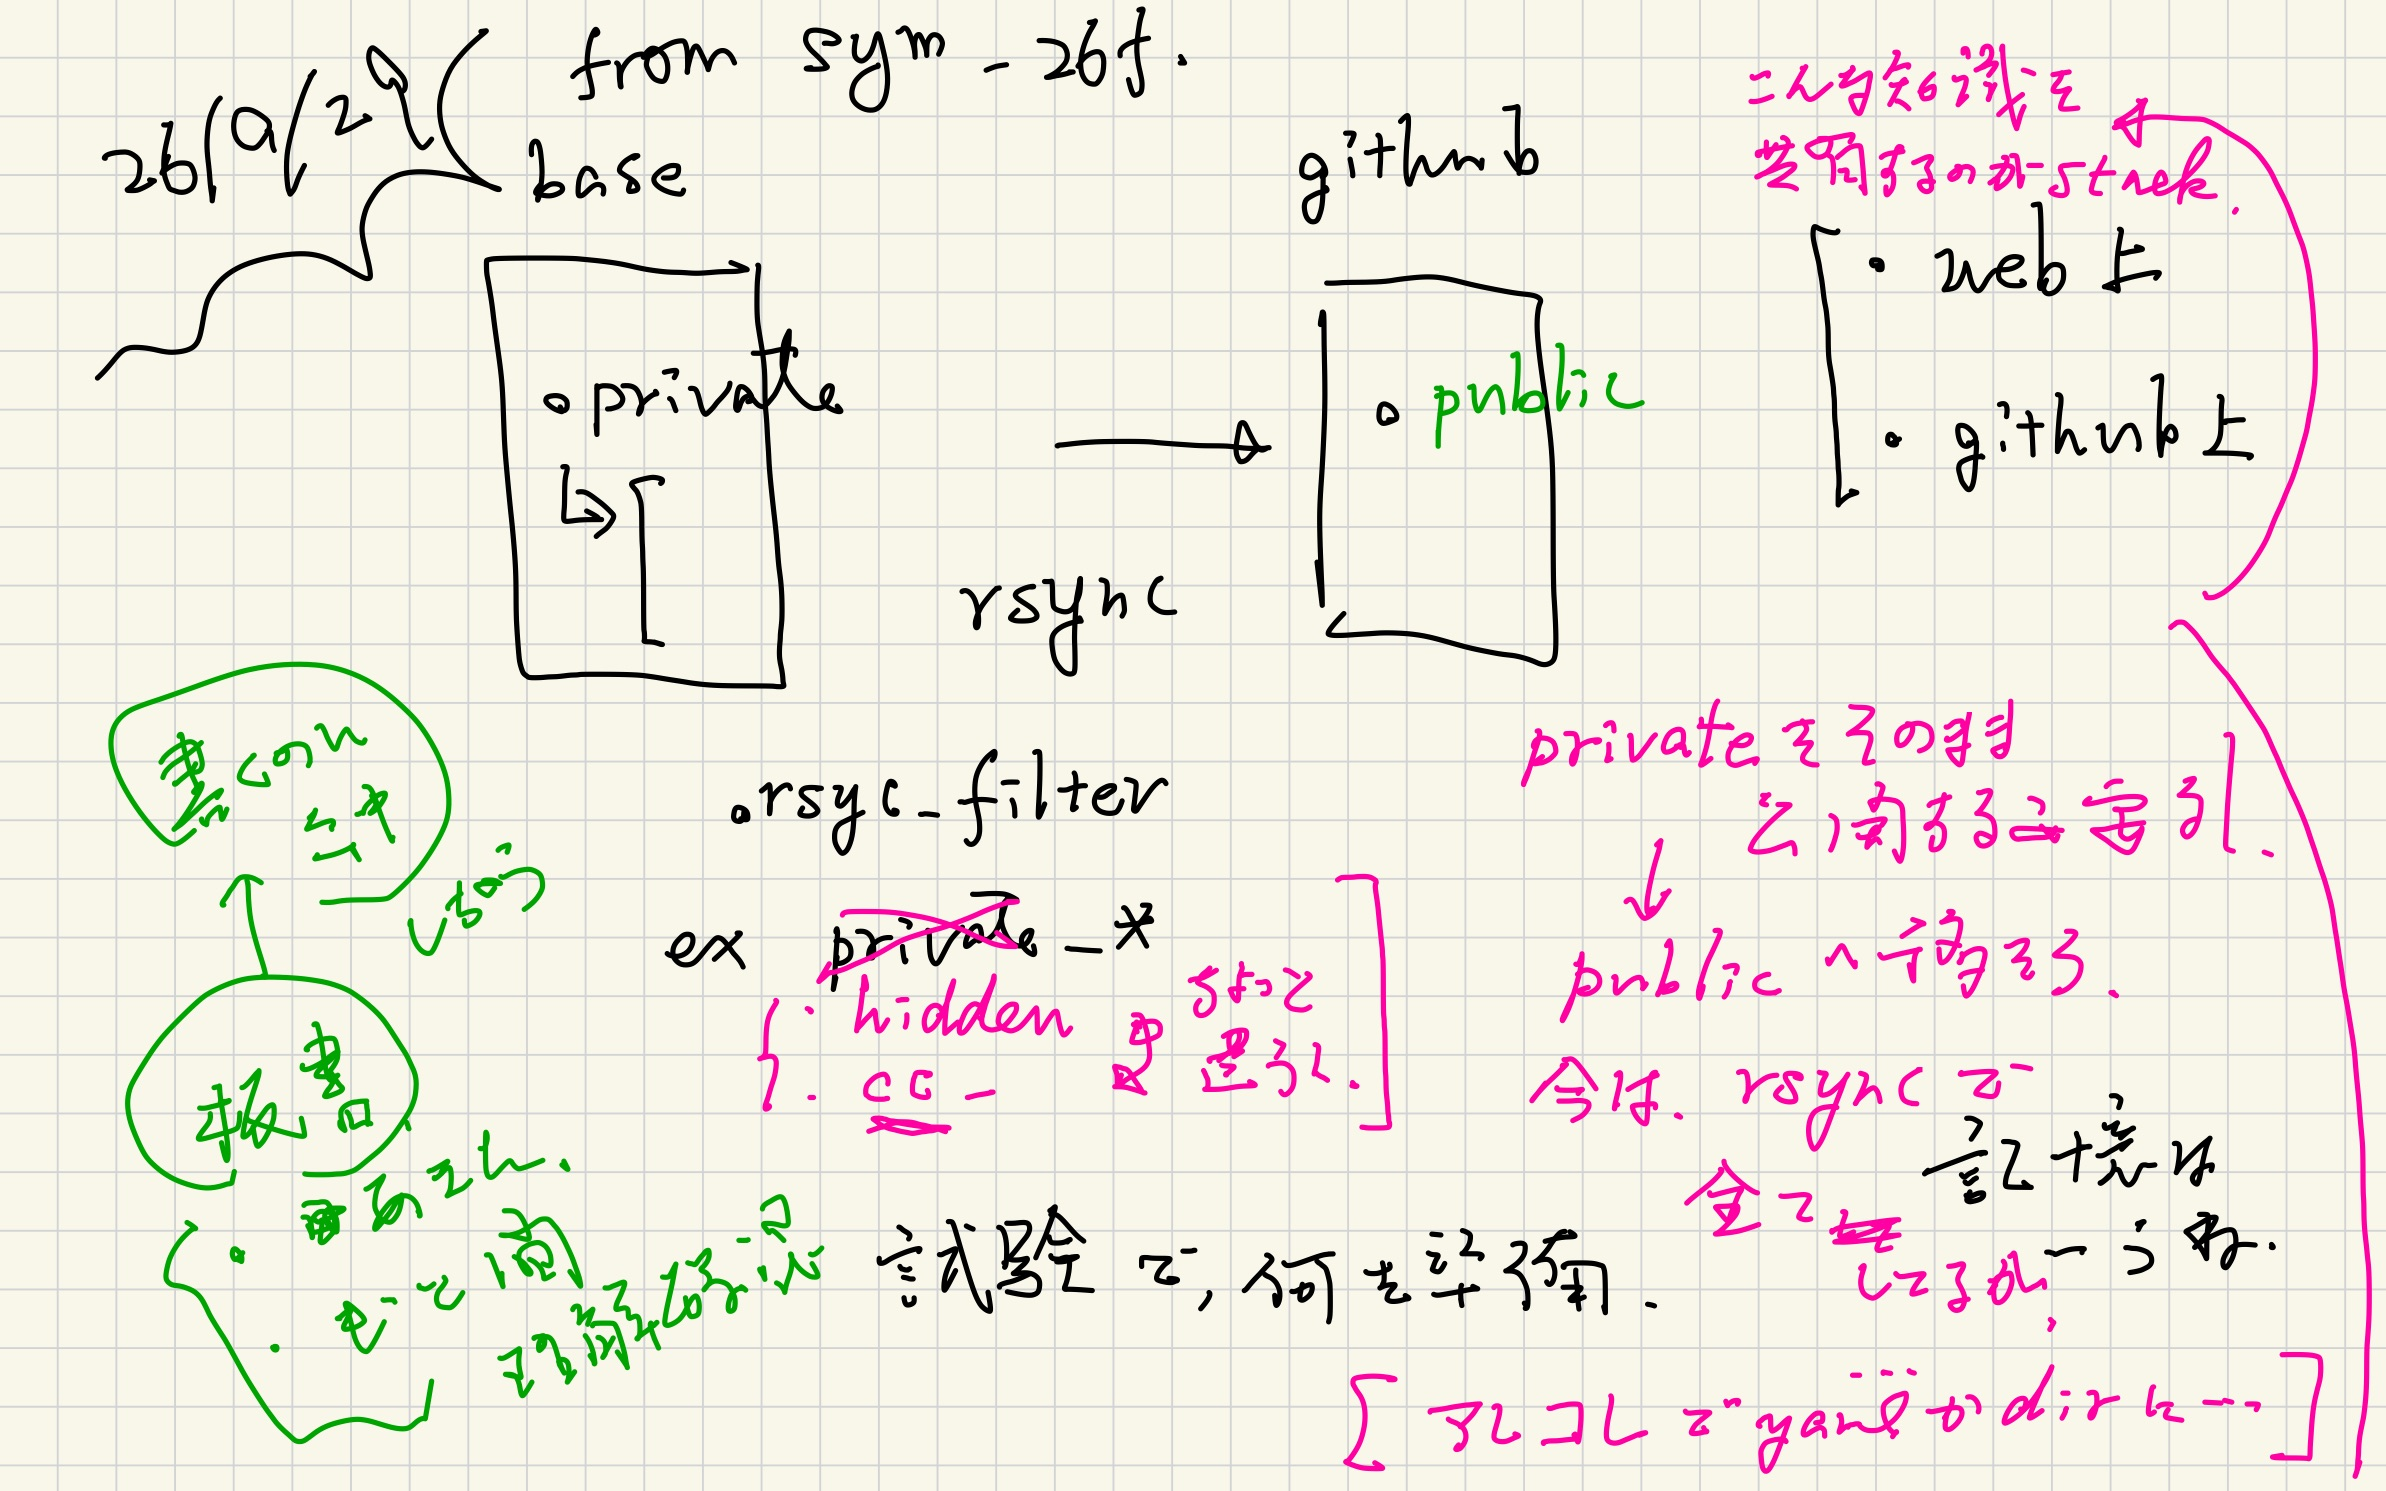
\includegraphics[width=\linewidth]{../d2_divide_chunk/figs/multi_scale_26f-9.jpg} & 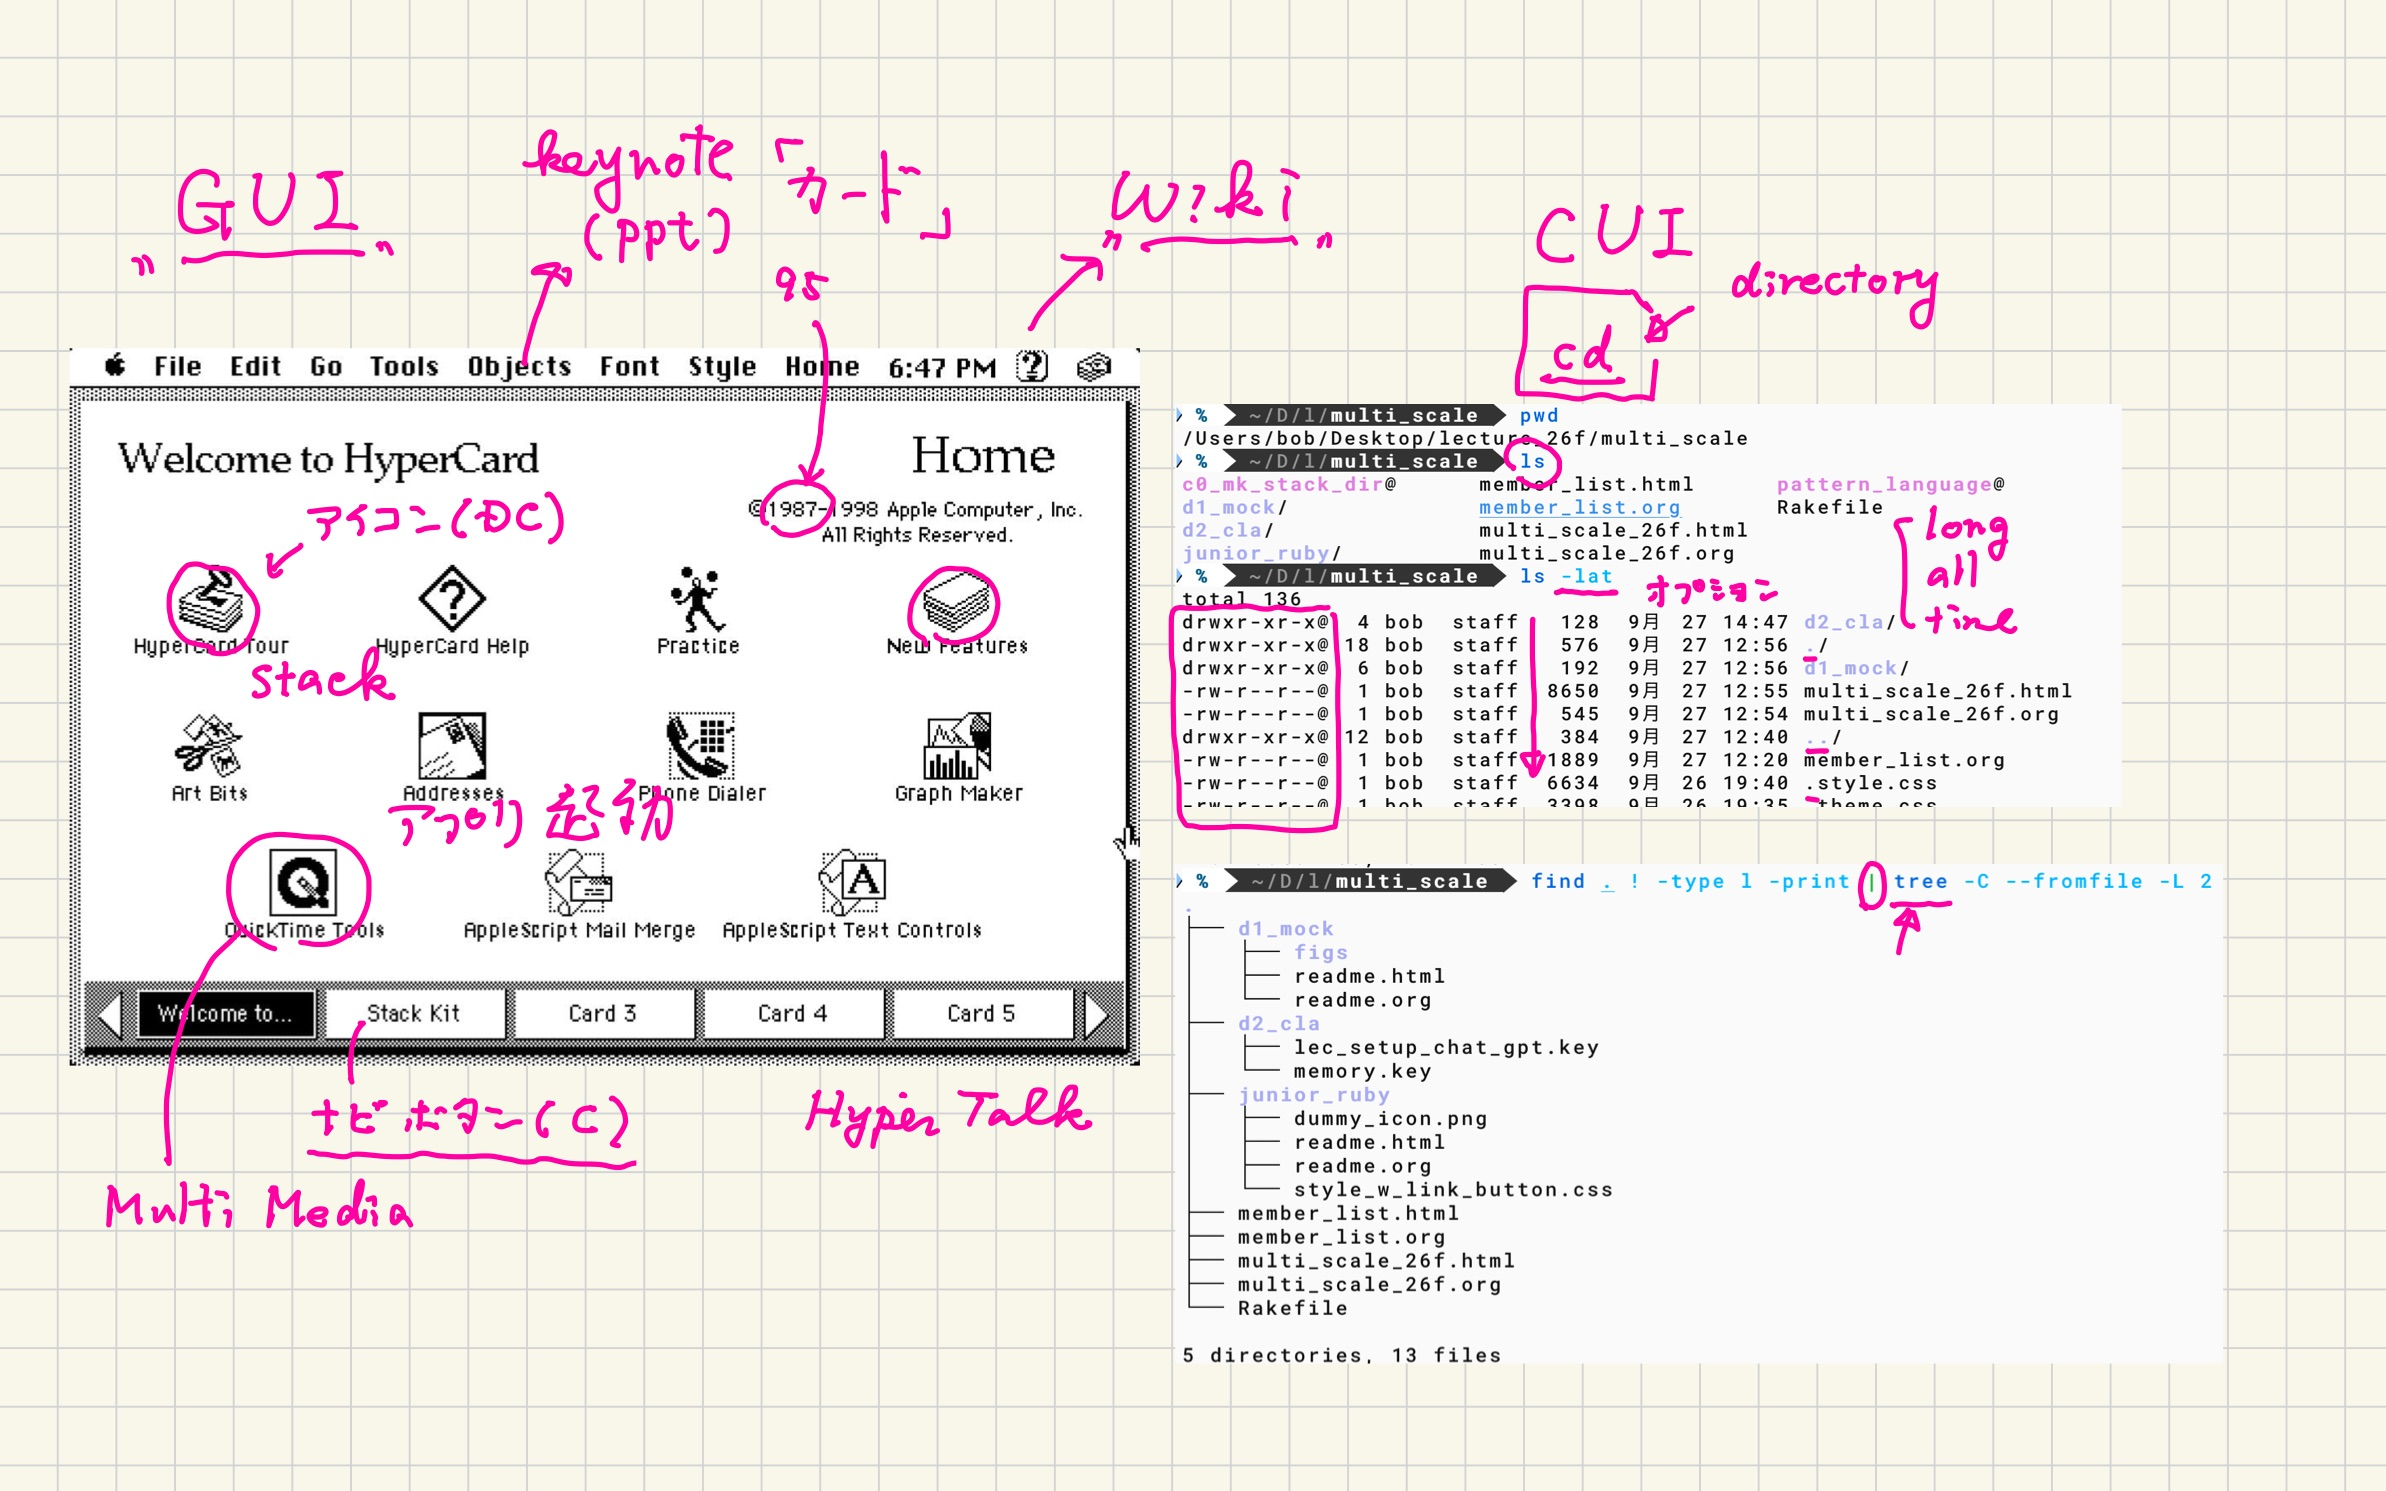
\includegraphics[width=\linewidth]{../d2_divide_chunk/figs/multi_scale_26f-10.jpg}\\
\end{tabular}
\end{center}
\section{Results}
\label{sec:org663d2cb}
\href{../d2\_divide\_chunk/readme.html}{prev\_button}
\href{../canvas.html}{up\_button}
\href{../d99\_junior\_ruby/readme.html}{next\_button}
\subsection{ppts}
\label{sec:orge8c1718}

HyperCardのMockが今見ていただいている
httpになります．

IconとかNaviとか，Actionが
GUIとCUIでどのように実現されているか
あるいはmockされているかを観察してください．

\begin{center}
\begin{tabular}{p{0.88\linewidth}}
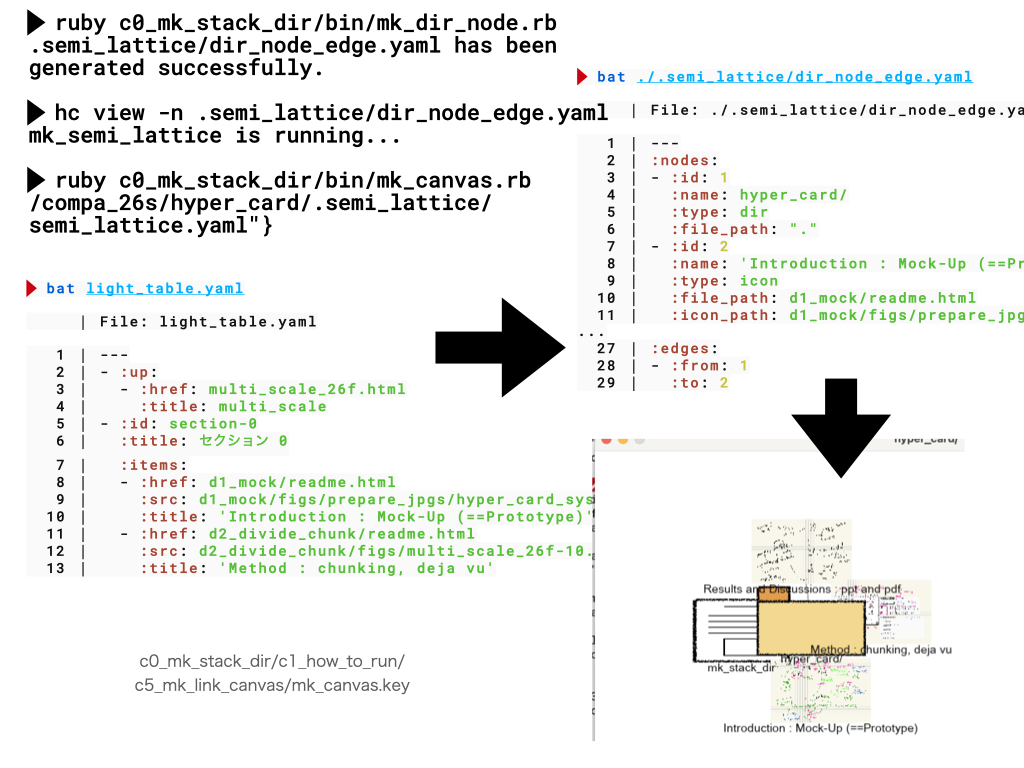
\includegraphics[width=\linewidth]{../d3_ppt_pdf/figs/mk_canvas.002.png}\\
\end{tabular}
\end{center}
\subsection{Pragmatic programmar (v2)}
\label{sec:orgcd63162}
なぜCUIがGUIよりプログラマに良いのかは，
次のテキストを参照ください．

\begin{itemize}
\item basic tool
\begin{itemize}
\item p3\_basic\_tools.pd
\item c16\_plain\_text.pdf
\item c17\_shell.pdf
\item c18\_editor.pdf
\item c19\_version\_github.pdf
\item c22\_note\_my\_help.pdf
\end{itemize}
\end{itemize}
\subsection{Why ruby?}
\label{sec:org4136fea}
さて，では，これらがどうやって実現されているか？
そしてeverday usersの手によってどのように
構築されるかを示すのが次の目的になります．

以下のテキストにはその必要性が書かれています．

\begin{itemize}
\item c21\_ruby.pdf
\item c51\_starter\_kit\_complete\_auto.pdf
\end{itemize}
\subsection{下書き(preparation notes)}
\label{sec:org6221b2e}
\begin{center}
\begin{tabular}{p{0.44\linewidth}p{0.44\linewidth}}
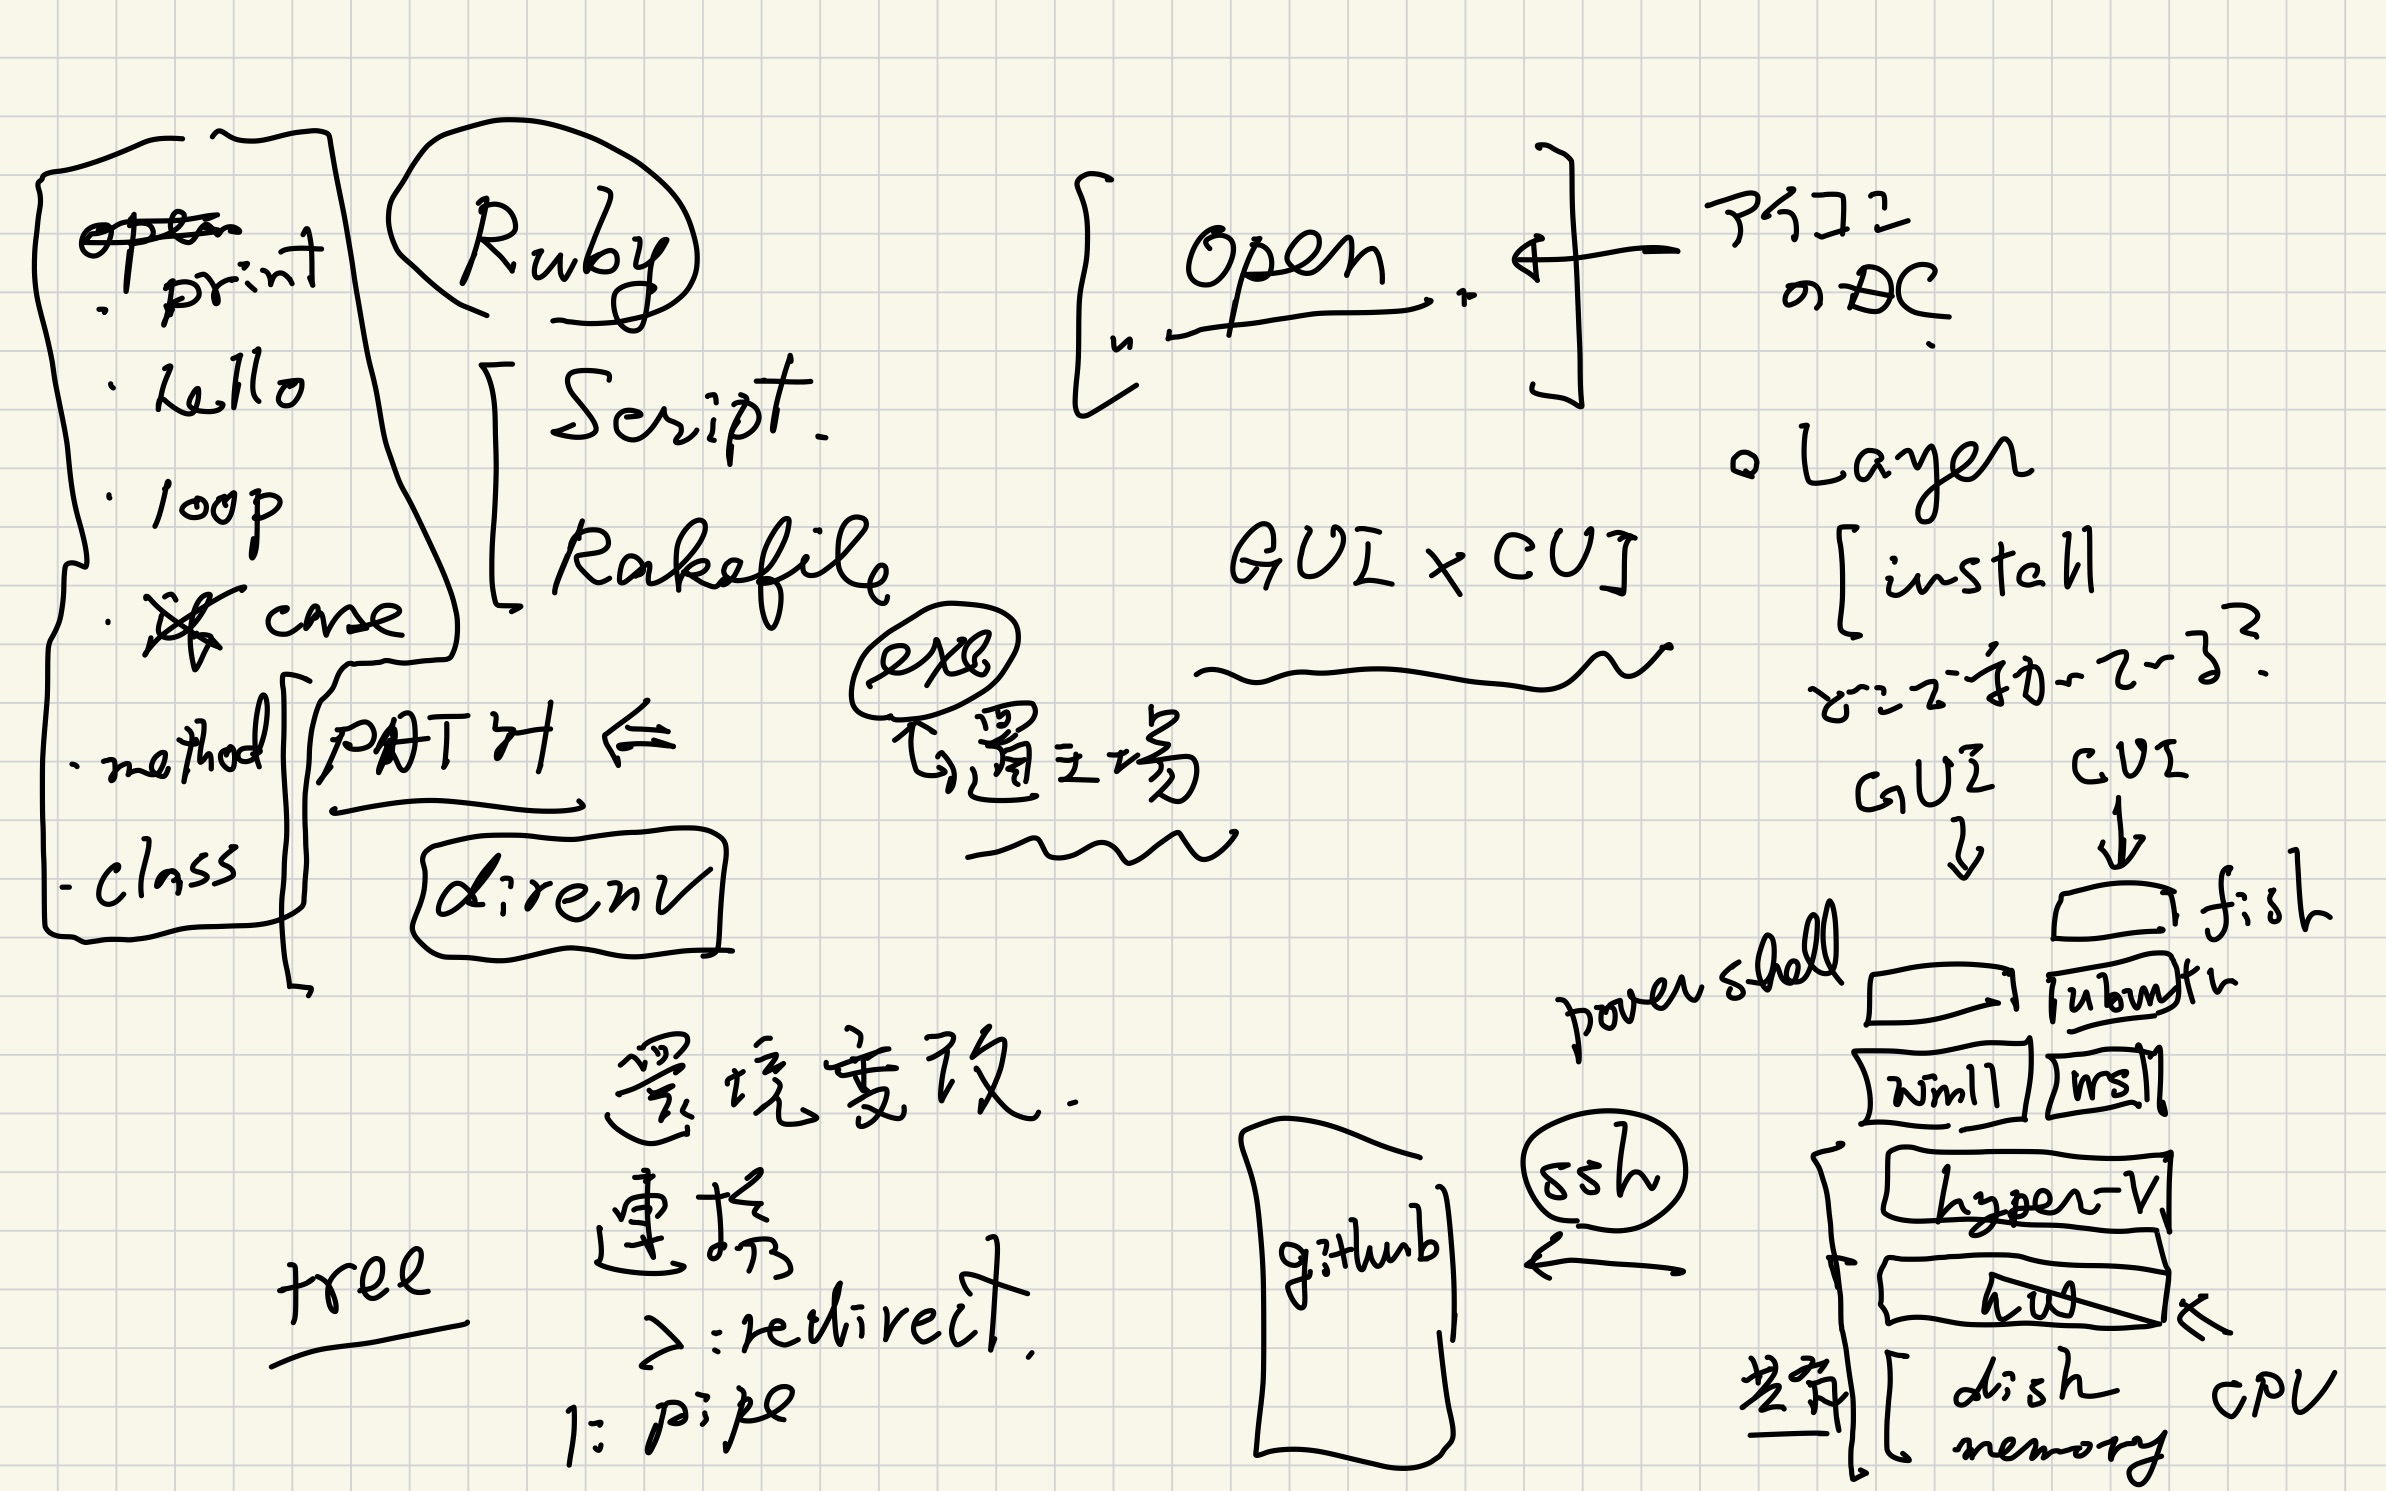
\includegraphics[width=\linewidth]{../d3_ppt_pdf/figs/multi_scale_26f-11.jpg} & 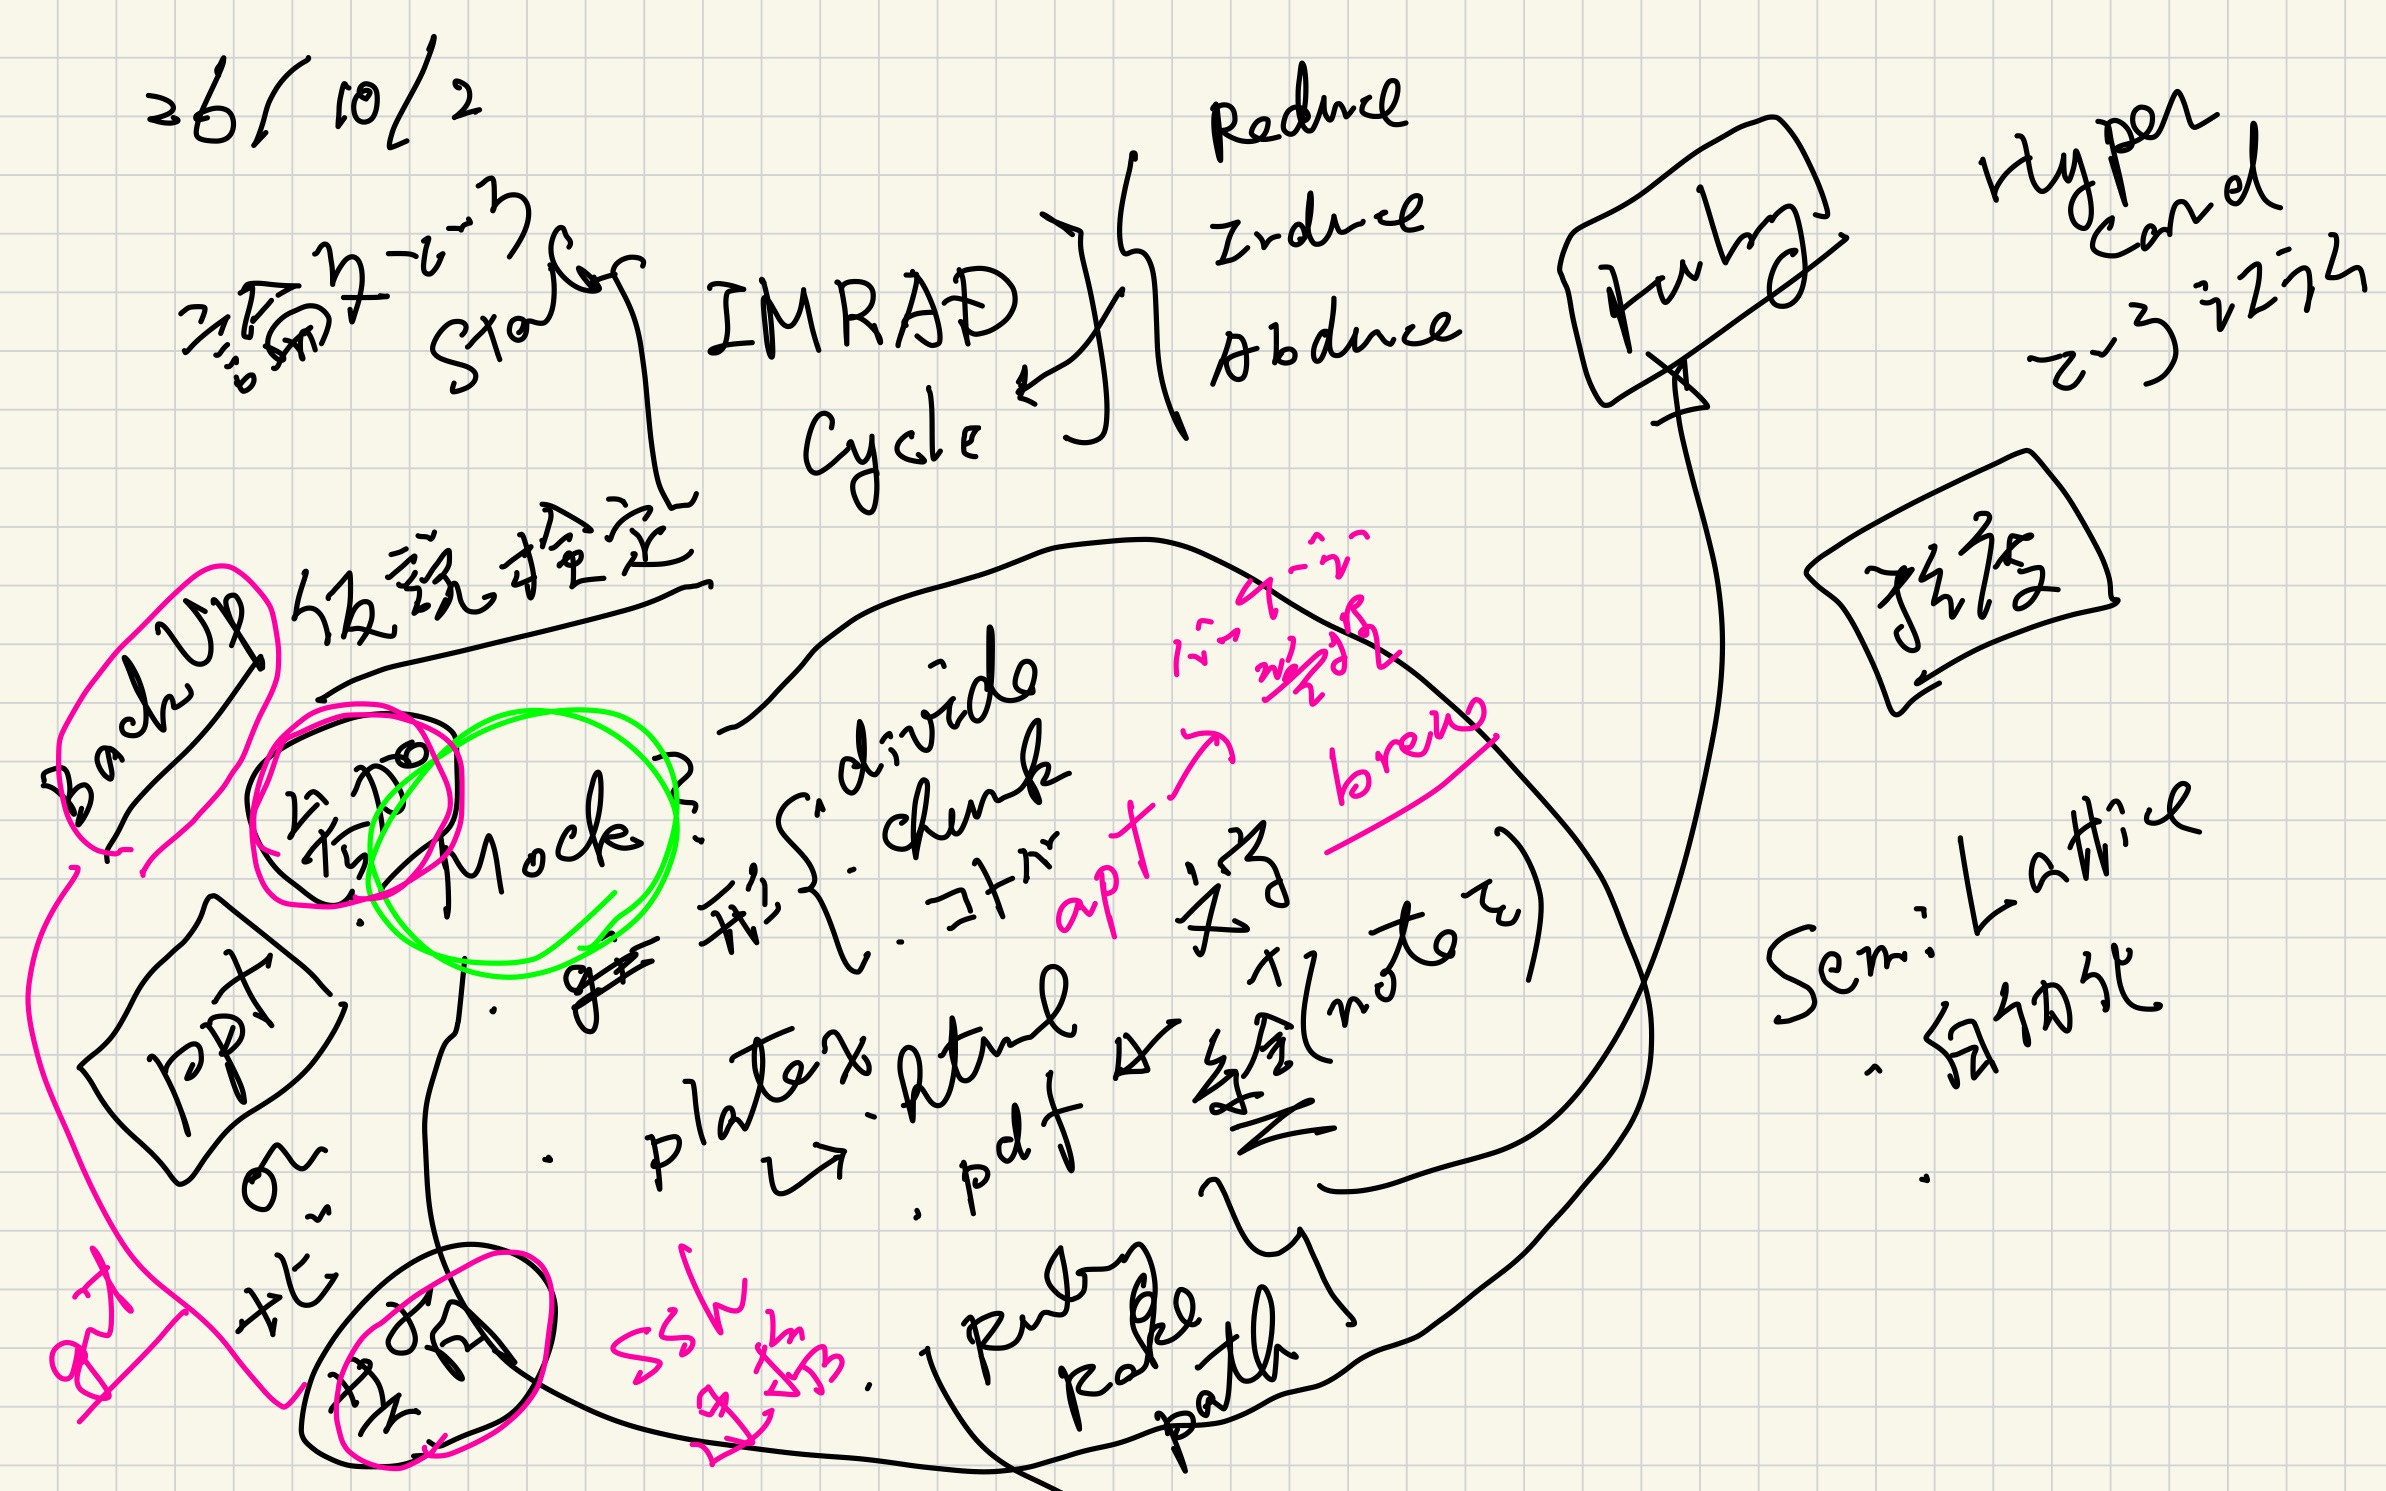
\includegraphics[width=\linewidth]{../d3_ppt_pdf/figs/multi_scale_26f-12.jpg}\\
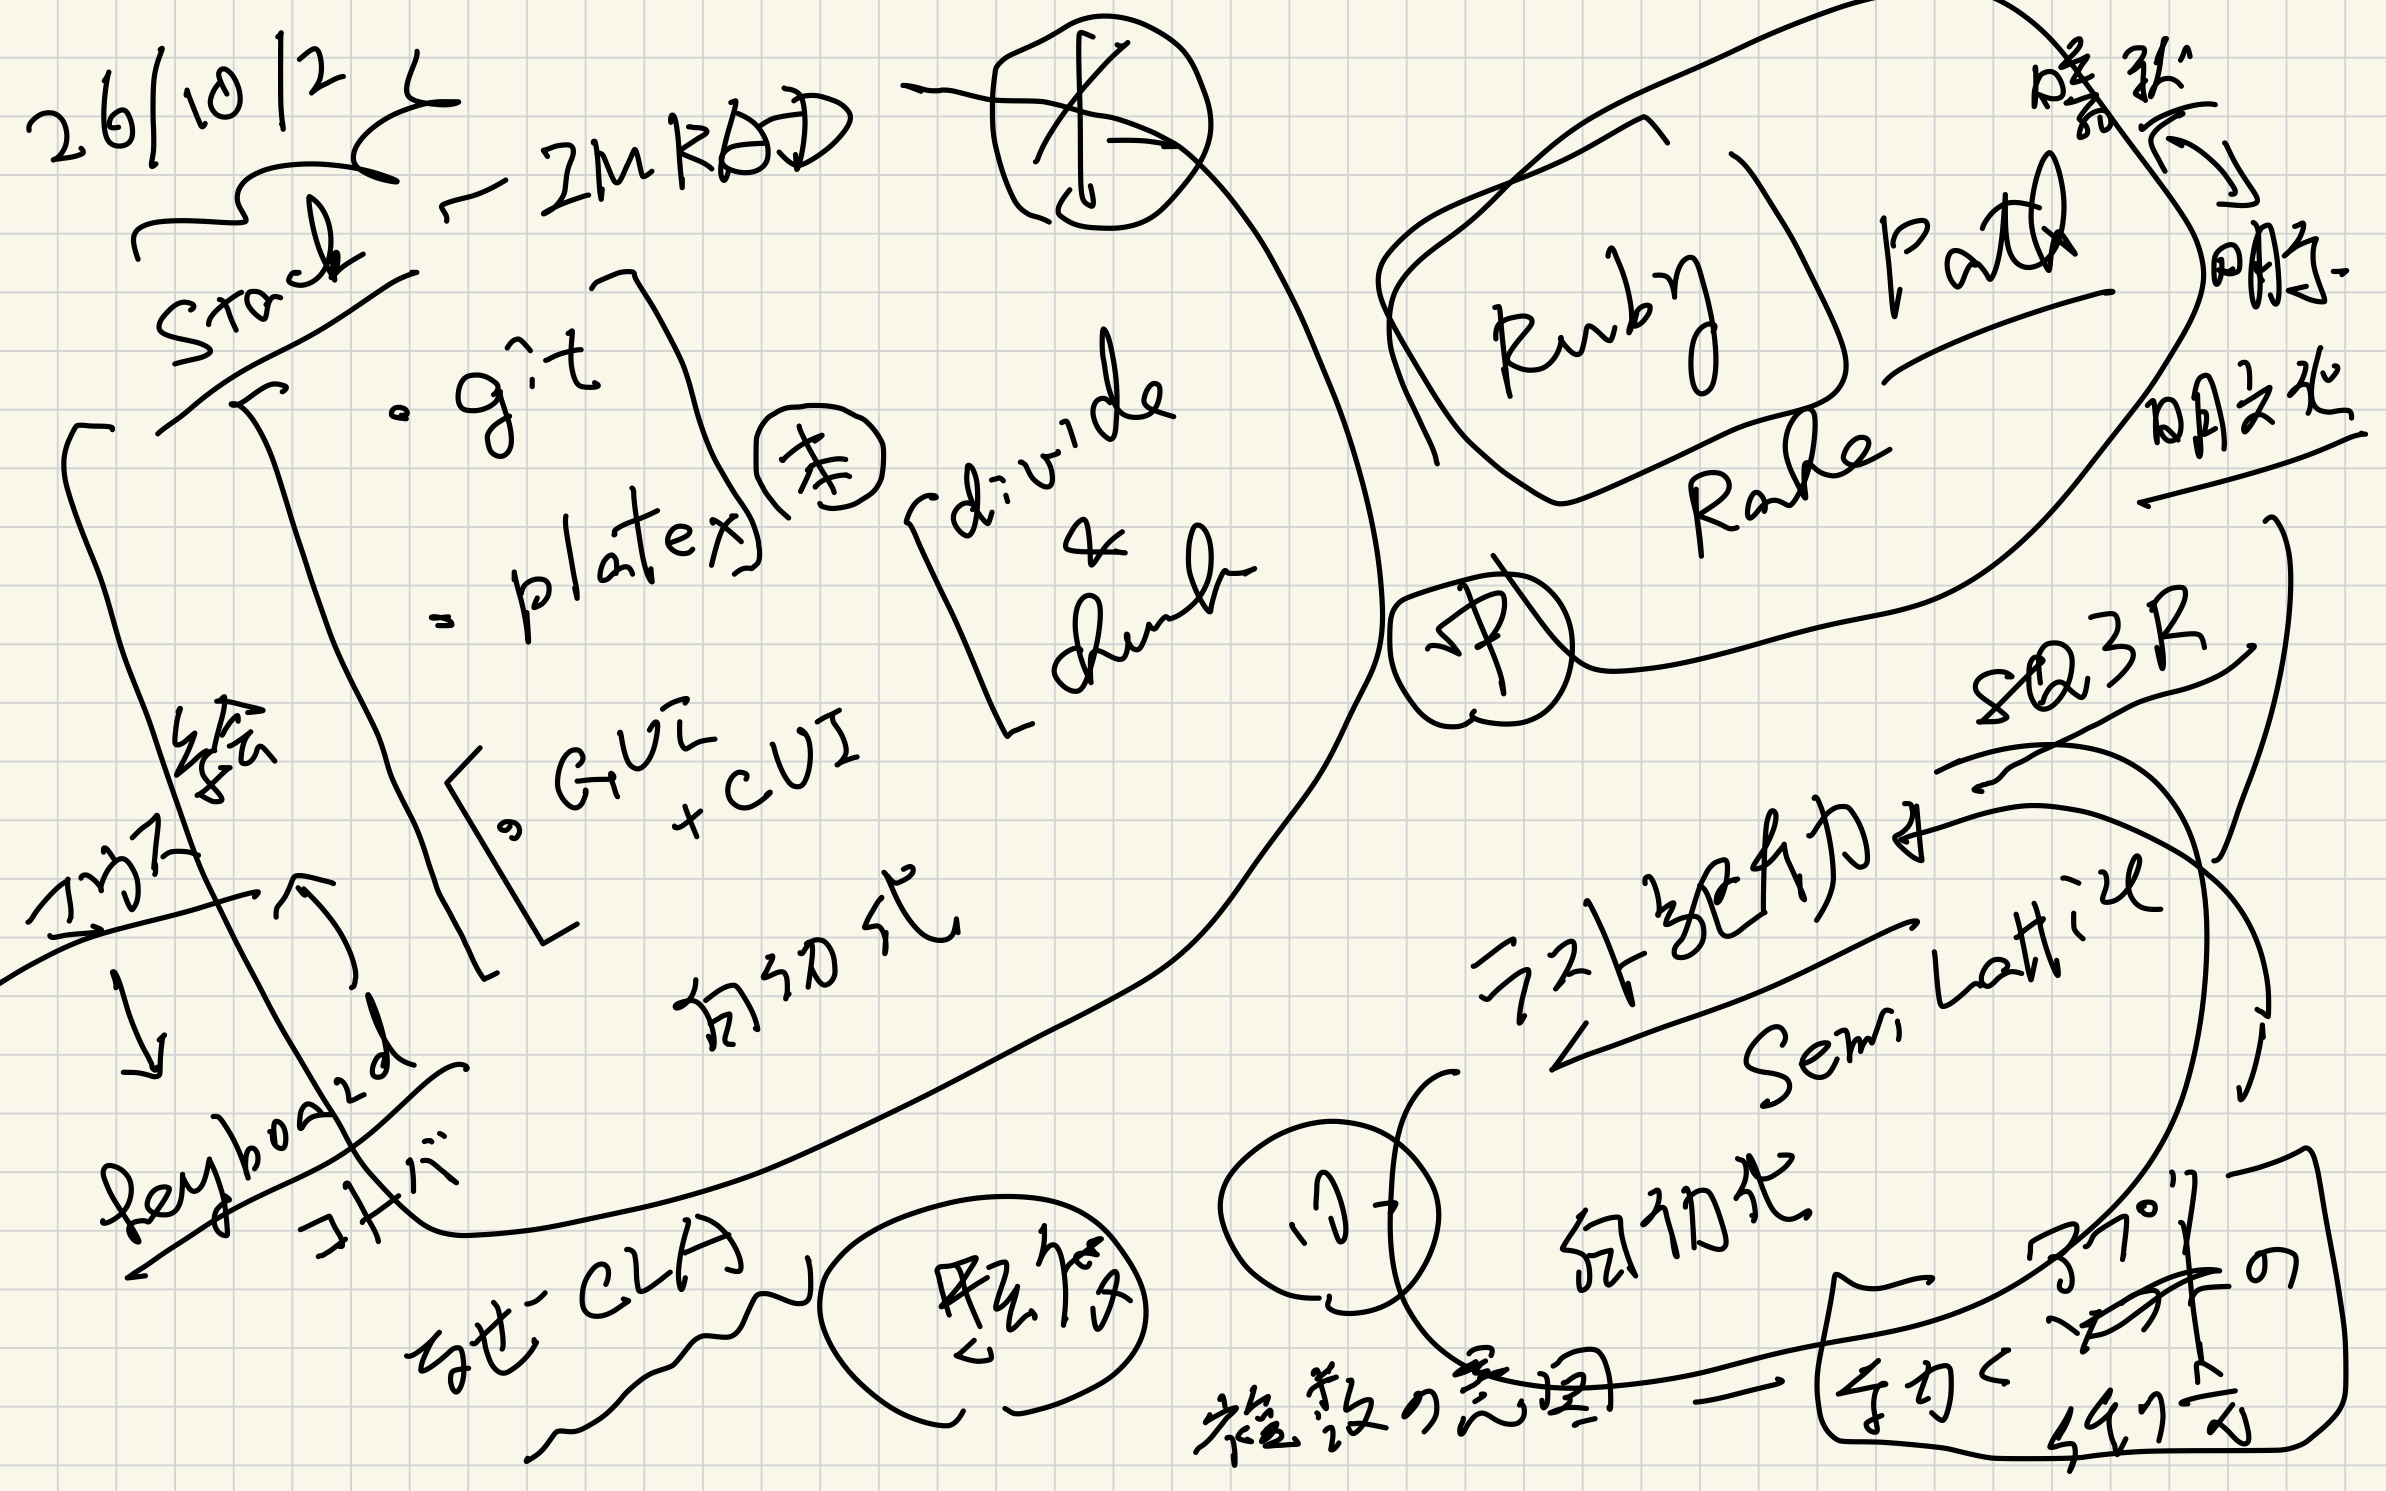
\includegraphics[width=\linewidth]{../d3_ppt_pdf/figs/multi_scale_26f-13.jpg} & 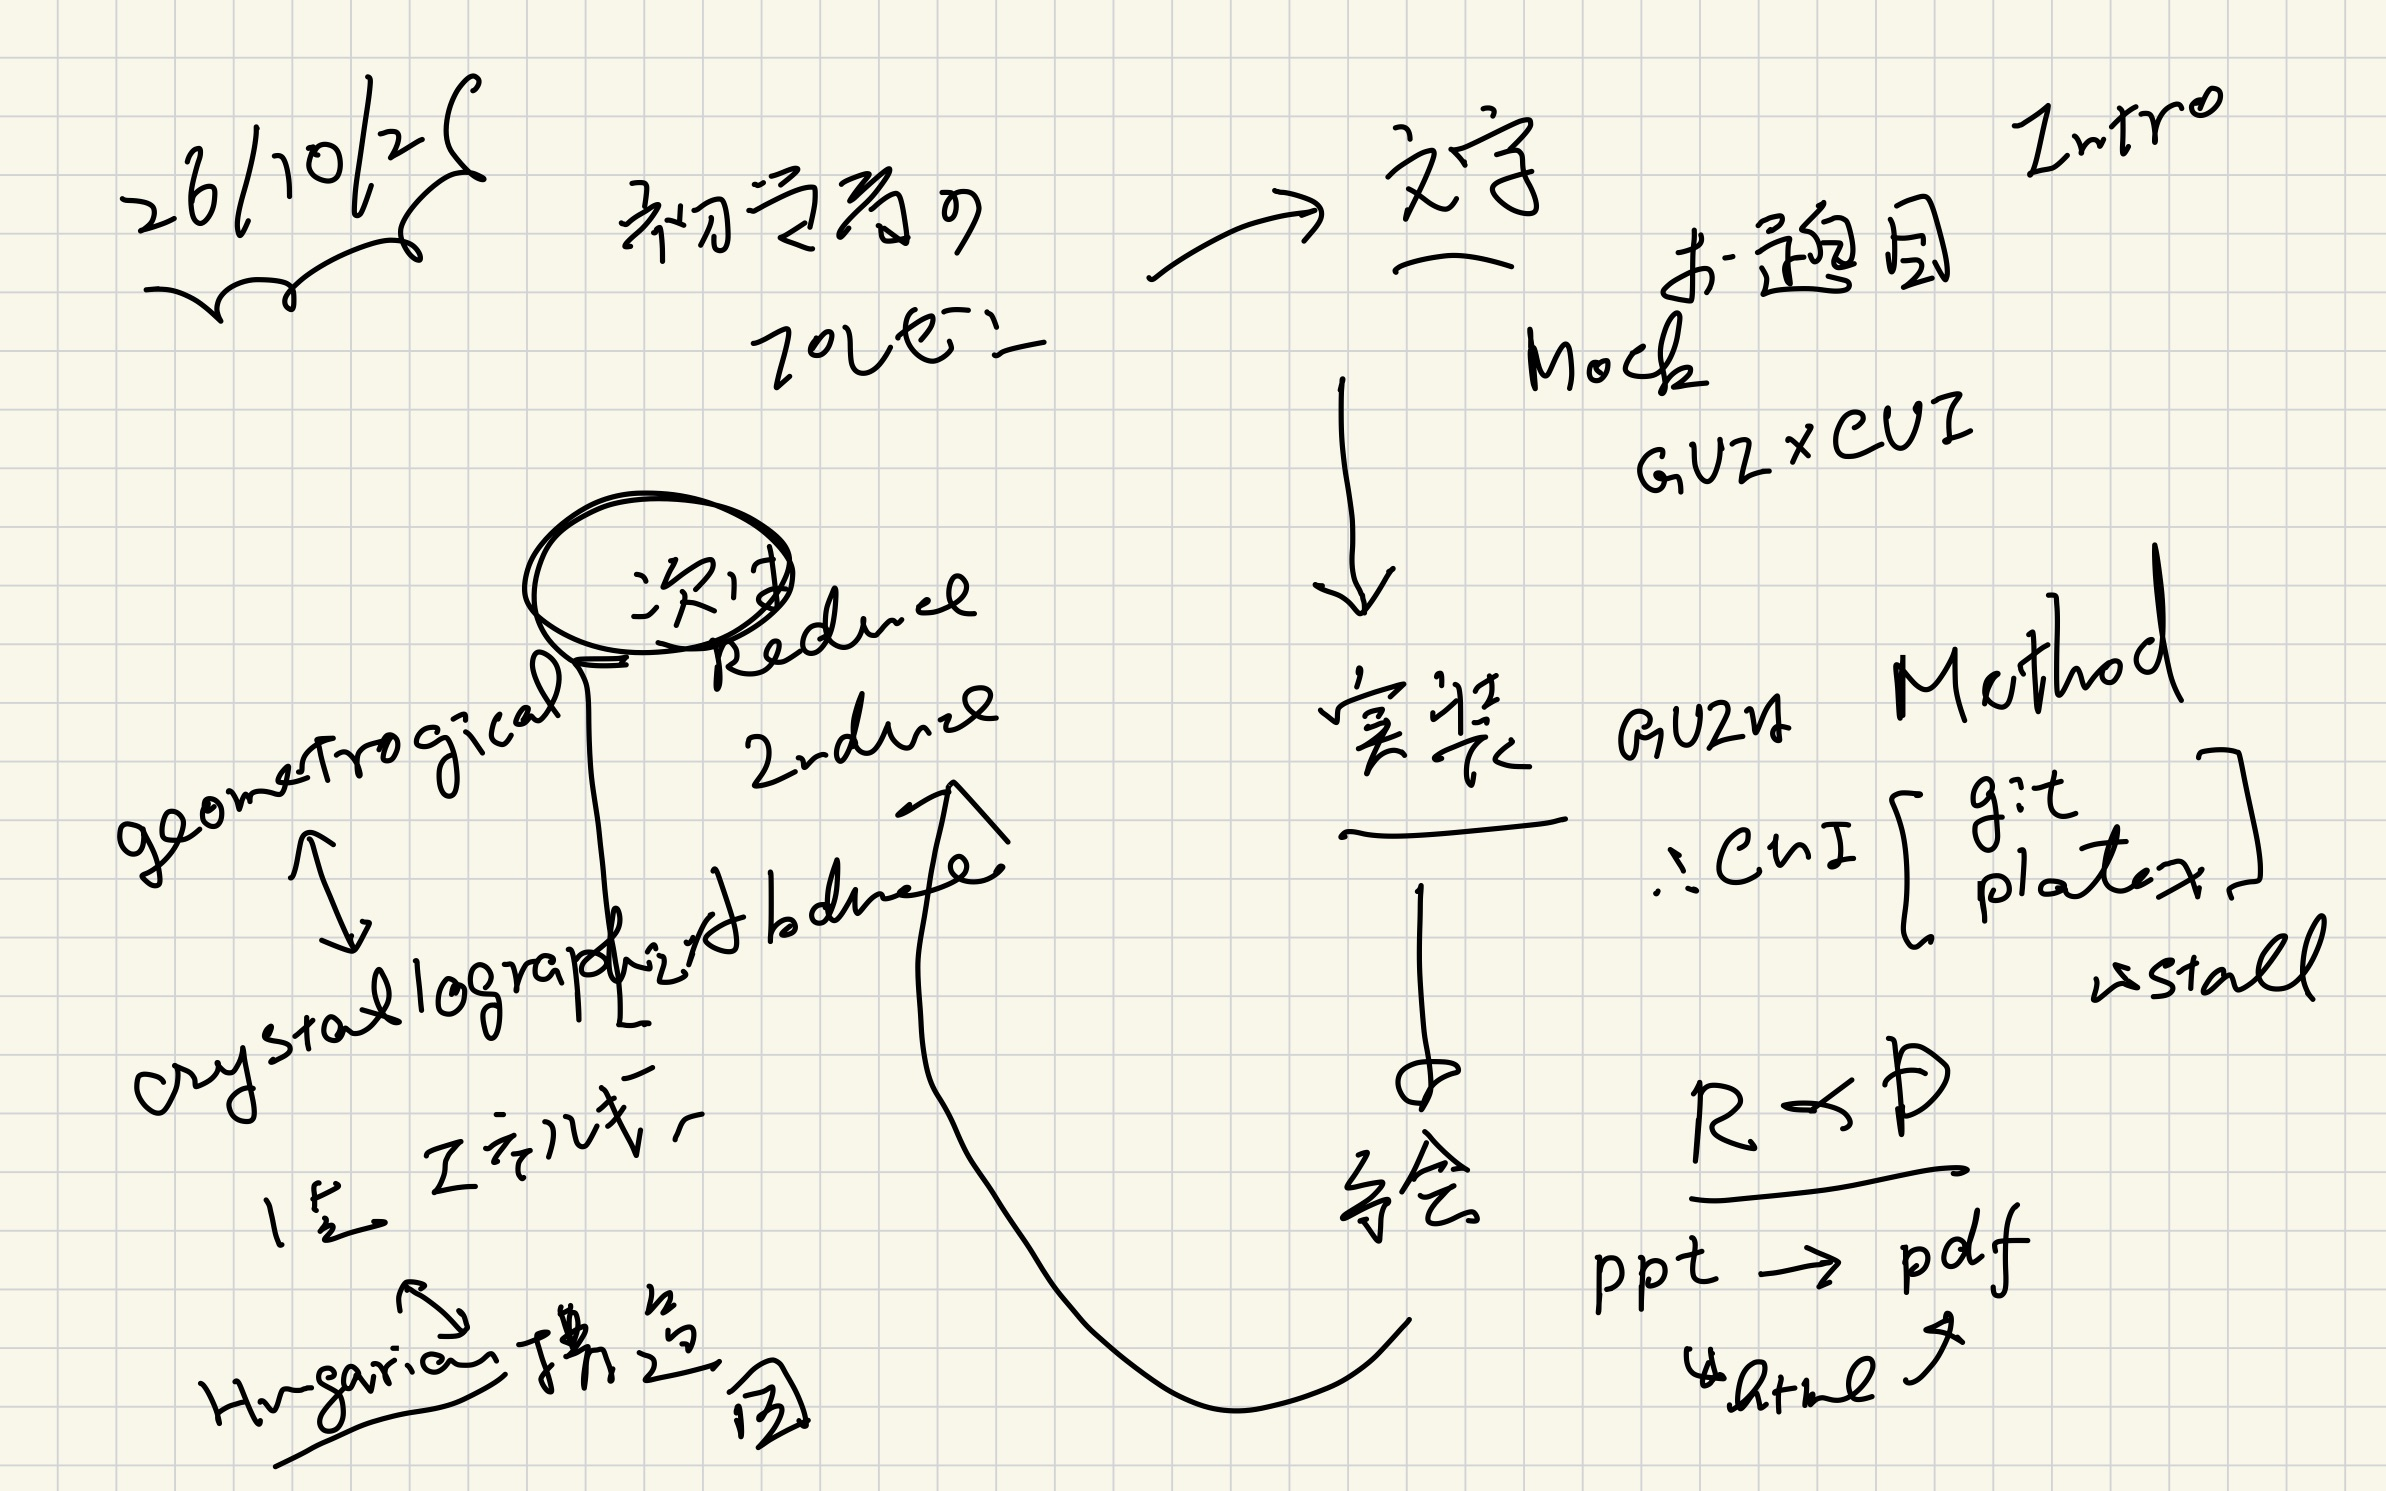
\includegraphics[width=\linewidth]{../d3_ppt_pdf/figs/multi_scale_26f-14.jpg}\\
\end{tabular}
\end{center}
\end{document}
